\chapter{DyMBO: Dynamic Mixture of Surrogate Models for Hyperparameter Optimisation}\label{ch:ch05:dymbo}



\section{Introduction}
\label{sec:ch05:intro}
The performance of machine learning (ML) and deep learning (DL) models crucially depends on how their hyperparameters are tuned~\citep{LavDav06,BisEtAl23}.
Tuning the hyperparameters in order to achieve peak performance of the model on  a specific task is challenging even for experts. 
This process is often addressed through trial-and-error methods, requiring significant effort and resources.
Hyperparameter optimisation (HPO) techniques alleviate this burden by automatically searching for well-performing hyperparameter configurations, removing the need for human intervention~\citep{SnoEtAl12}.
While automated HPO techniques have shown great potential for classical ML models~\citep{SnoEtAl12,FeuEtAl22}, they are not as easily applicable to more complex ML and DL domains, where evaluating a single configuration of a model can be very expensive~\citep{BroEtAl20}.
Moreover, due to the lack of access to an explicit problem formulation, HPO is handled as a black-box problem.
Consequently, all automated HPO techniques rely on the only available information about the problem, \emph{i.e.}, evaluating the quality of candidate configurations, to steer the search towards the most promising regions of the search space and a good estimate of the global optimum.
% \changed{
Throughout this article, we consider HPO in the batched setting, in which $k$ candidate configurations are proposed and evaluated per BO iteration, as is standard practice in large-scale HPO~\citep{CowEtAl22,BisEtAl23}.
% }

Bayesian optimisation (BO)~\citep{Mockus12,Garnett23,Frazier18,Kushner62,Kushner64} is a surrogate-based, sample-efficient approach for global optimisation of expensive-to-evaluate black-box problems.
BO is particularly well-suited for settings with a very limited budget of available evaluations (relative to the size of the search space), such as HPO.
Various BO-based HPO techniques have been developed and successfully applied to this end; a prominent example is 
HEBO~\citep{CowEtAl22}, the winner of the NeurIPS BBO competition~\citep{TurEtAl20}.
One of the key components of BO is a 
% probabilistic \er{here, see comment below} 
\emph{surrogate model}, which is built on an initial sample of candidate solutions to approximate the objective function while also quantifying its uncertainty.
% \changed{
% In the sequential version of the BO algorithm, at each iteration 
At each iteration of BO, new candidate solutions are selected to be evaluated next by means of maximising an acquisition function defined on the surrogate.
% }
% At each iteration a new solution candidate is selected to be evaluated next by means of maximising an acquisition function defined on the surrogate.
The surrogate is then iteratively refined with newly observed candidate solutions, until the total budget of available evaluations has been exhausted.
% \er{I would be fine to revert it to the previous version, but then we need to say ``one or multiple solution candidates are selected"}
%
Fitting the surrogate model to the observed data is a prediction task that often involves probabilistic models. 
% \er{Since it \textit{often} involves probabilistic models, then I would remove the word ``probabilistic" above.}
BO then uses these probabilistic predictions of function values across the search space to guide the search towards a good estimate of the global optimum.
% \er{I'd start a new paragraph here and remove the ``thus", as this is the precise research challeng we address} 

% \changed{
The choice of the surrogate model strongly affects BO performance and is often linked to the dimensionality of the problem at hand and the nature of the corresponding search space.
% }
For continuous search spaces, Gaussian processes (GPs)~\citep{RasWil06} are the most widely adopted surrogate model and tend to be particularly effective in continuous search spaces~\citep{EggEtAl13,EggEtAl21,BenEtAl25}.
On the other hand, random forests (RFs)~\citep{Breiman01} as surrogate models natively support discrete and conditional search spaces, and tend to excel in higher problem dimensionalities, where GPs suffer from prohibitive computational complexity and reduced accuracy due to the increased volume of the search space
% search space volume
% \er{where GPs suffer from prohibitive computational complexity and reduced accuracy due to the increased search space volume}
~\citep{EggEtAl13,JenEtAl17,LiEtAl18}.
For complex HPO tasks in mixed domains, with numerical, ordinal and categorical hyperparameters, it is highly desirable to leverage the complementary strengths of inherently different surrogate models.
One natural way to achieve this is via ensemble methods, which have demonstrated their versatility in the context of BO-based HPO techniques for treating a wide range of heterogeneous problems~\citep{TurEtAl20,HofEtAl11}.
% \hh{the following didn't flow well and was rather unclear, so I've changed it a bit -- check carefully:}
% Here, we tackle complex HPO search spaces directly through adaptive choice of the most suitable surrogate model. 

% In conjunction with BO-based HPO techniques, multi-fidelity approaches~\citep{LiEtAl2017,LiEtAl20,FalEtAl2018,AwaEtAl21} have been widely used to address expensive HPO problems, due to the fact that they use cheap approximations of the target function at hand.
% \changed{
% However, they are not in scope of our work presented here, as they are conceptually different to the direction followed here, as they do not take into consideration the nature of the search space, but rather use low-fidelity evaluations as a proxy for full-fidelity evaluations to allow for the better use of the available budget.
% }
% \hh{I wonder about these last two arguments. Why should anyone care whether their working mechanisms differ if they address/solve the same problem? Which also begs the question why they would be out of scope ... perhaps it would be safer to say they are conceptually orthogonal to the direction followed here, as they do not take into consideration ..., but rather ... Then, a combination of our approach with multi-fidelity techniques could be an interesting direction for future work.}
% \todo{add references to multi-fidelity literature here and say it is out of scope of discussion for this paper}


\begin{figure}
    \centering
    % \includegraphics[width=\textwidth]{figs/Flowchart_ensemble-5.pdf}
    \resizebox{\textwidth}{!}{%
    \begin{tikzpicture}[
        >=stealth,
        myybox/.style={rectangle, rounded corners, draw=black, thick, fill=myyellow, align=center, text width=2.8cm, minimum height=1.8cm, font=\small\bfseries},
        myrbox/.style={rectangle, rounded corners, draw=black, thick, fill=mypink, align=center, text width=2.8cm, minimum height=1.8cm, font=\small\bfseries},
        mybbox/.style={rectangle, rounded corners, draw=black, thick, fill=mypurple, align=center, text width=2.6cm, minimum height=1.8cm, font=\small\bfseries},
        mydiamond/.style={diamond, draw=black, thick, fill=black, text=white, align=center, aspect=1.5, font=\small\bfseries, inner sep=2pt}
    ]
    
    % Group 1: Init
    \draw[fill=mygray, draw=mygray, rounded corners, thick] (-1.8, -2.2) rectangle (1.8, 2.2);
    \node[myybox, minimum height=1.4cm] (init1) at (0, 1.1) {Initial Design};
    \node[myrbox, minimum height=1.4cm] (init2) at (0, -1.1) {Weight\\Initialisation};
    
    % Group 2: Surrogate Model Fitting
    \draw[fill=mypinkbg, draw=mypinkbg, rounded corners, thick] (2.4, -1.6) rectangle (6.2, 2.5);
    \node[myybox, minimum height=2.0cm, text width=2.6cm] (surrn) at (4.7, 1.1) {};
    \node[myybox, minimum height=2.0cm, text width=2.6cm] (surr2) at (4.4, 0.6) {};
    \node[myybox, minimum height=2.0cm, text width=2.6cm] (surr1) at (4.1, 0.1) {Surrogate\\Model\\Fitting};
    \node[anchor=north east, font=\scriptsize] at ([shift={(-0.1,-0.1)}]surrn.north east) {Model $m$};
    \node[anchor=north east, font=\scriptsize] at ([shift={(-0.1,-0.1)}]surr2.north east) {Model 2};
    \node[anchor=north east, font=\scriptsize] at ([shift={(-0.1,-0.1)}]surr1.north east) {Model 1};
    
    \coordinate (c1) at (1.8, 0);
    \coordinate (c2) at (2.4, 0);
    \draw[->, thick] (c1) -- (c2);
    
    % Group 3: Model Ensemble
    \node[myrbox, text width=2.6cm] (ens) at (8.5, 0) {Model\\Ensemble/\\Selection};
    \draw[->, thick] (6.2, 0) -- (ens.west);
    
    % Group 4: AFO
    \node[myybox, text width=2.6cm] (afo) at (12.3, 0) {Acquisition\\Function\\Optimisation\\($k$ samples)};
    \draw[->, thick] (ens.east) -- (afo.west);
    
    % Group 5: Sample Eval
    \node[myybox, text width=2.6cm] (seval) at (16.1, 0) {Sample\\Evaluation\\and\\Optimum\\Update};
    \draw[->, thick] (afo.east) -- (seval.west);
    
    % Group 6: Accuracy Eval
    \node[myrbox, minimum height=2.0cm, text width=2.6cm] (accn) at (20.5, 1.1) {};
    \node[myrbox, minimum height=2.0cm, text width=2.6cm] (acc2) at (20.2, 0.6) {};
    \node[myrbox, minimum height=2.0cm, text width=2.6cm] (acc1) at (19.9, 0.1) {Accuracy\\Evaluation};
    \node[anchor=north east, font=\scriptsize] at ([shift={(-0.1,-0.1)}]accn.north east) {Model $m$};
    \node[anchor=north east, font=\scriptsize] at ([shift={(-0.1,-0.1)}]acc2.north east) {Model 2};
    \node[anchor=north east, font=\scriptsize] at ([shift={(-0.1,-0.1)}]acc1.north east) {Model 1};
    
    \draw[->, thick] (seval.east) -- (18.6, 0); 
    
    % Group 7: Model Weight Assign
    \node[myrbox, text width=2.6cm] (weight) at (24.3, 0) {Model Weight\\Assignment\\($w=1$ to best,\\$0$ otherwise)};
    \draw[->, thick] (21.7, 0) -- (weight.west); 
    
    % Group 8: EMA
    \node[myrbox, text width=2.6cm] (ema) at (28.1, 0) {Exponential\\Moving\\Average of\\model weights};
    \draw[->, thick] (weight.east) -- (ema.west);
    
    % Loop back from EMA top to Model Ensemble
    \draw[->, thick, dotted] (ema.north) -- ++(0, 2.0) -| (ens.north);
    
    % Budget Check logic
    \node[mydiamond] (budget) at (21, -4.5) {Budget\\exhausted?};
    \node[myybox, text width=2.6cm] (sampup) at (16.1, -4.5) {Sample Set\\Update with\\new samples};
    \node[mybbox] (ret) at (25.5, -4.5) {Return solution};
    
    \draw[->, thick] (ema.south) -- ++(0, -1.5) -| (budget.north);
    
    \draw[->, thick] (budget.west) -- node[above, font=\small\bfseries] {No} (sampup.east);
    \draw[->, thick] (budget.east) -- node[above, font=\small\bfseries] {Yes} (ret.west);
    
    \draw[->, thick] (sampup.west) -| (4.1, -1.6); 
    \end{tikzpicture}%
    }
    \caption{
    % \changed{
    Bayesian optimisation pipeline with dynamic ensembling and selection of surrogate models (\texttt{DyMBO}). In red, the blocks for the ensembling and selection strategy that have been plugged into the standard BO procedure. 
    % }
    We start by sampling an initial set of hyperparameter configurations and initialising the weights for surrogate models used to construct the ensemble. Within the BO loop, all surrogates are separately fitted to the past observations and then combined in the weighted ensemble, 
    which can be composed of only a single surrogate in case of greedy selection. The acquisition function is derived from the model ensemble and optimised to determine the next points to sample. The target function is evaluated on the points identified by optimising the acquisition function. The accuracy of the surrogate models is then evaluated on all sampled points, and surrogates are assigned new weights. Finally, the weighting scheme for the next iteration is obtained via an exponential moving average between the old and new weights, which is parametrised by a smoothing factor $\alpha$ in order to determine how much historical information is retained: 
    % \changed{
    the weighted ensemble is reconstructed if $\alpha < 1$ or the single most accurate surrogate is selected if $\alpha = 1$.
    % }. 
    % \todo{mark explicitly where sample evaluation is happening}
    }
    
    \label{fig:ch05:diagram}
\end{figure}

% \changed{
We propose a novel approach to enhance BO-based HPO performance by dynamically tailoring the surrogate model(s) during the optimisation process.
Our approach, dubbed \texttt{DyMBO}, dynamically adjusts the influence of multiple surrogate models used at each BO iteration, ranging from a weighted ensemble of complementary surrogates to a selection of a single best-performing surrogate.
To this end, \texttt{DyMBO}
assigns the largest weight to the surrogate model with the highest accuracy
on all observed points up to the current BO iteration and updates the 
weights via exponential moving average (see~\cref{fig:ch05:diagram} for details).
We use the term
% \hh{add: the term} 
\emph{ensemble} for the regime in which multiple surrogates retain non-zero weight, and \emph{selection} for the special case in which the weighting collapses to a single retained surrogate at each iteration.
% }

% \changed{
In particular, we present, for the first time, a dynamic tailoring approach to surrogate model combination and selection in the context of HPO. 
% }
This poses a significant challenge, as there is a trade-off between the time needed for finding the best hyperparameter configuration and the time complexity of target function evaluations (\emph{i.e.}, if the optimiser requires more time to determine the next configurations to sample, there is naturally less time available for evaluating the target function).
In the context of HPO, evaluating the target function means evaluating the performance of a given ML model for a given hyperparameter configuration on a given dataset.
Ensembling approaches in general require training and querying more than one surrogate model, which leads to more time required for the optimisation phase.
We assess the effectiveness of \texttt{DyMBO} %our dynamic surrogate ensembling 
on various HPO tasks involving numerous datasets and machine learning models. 
To this end, we compare \texttt{DyMBO} to several single-surrogate-based BO baselines and a range of competitive HPO frameworks, and we show that our method achieves a better average ranks than all other considered methods across both cheap and expensive functions in terms of time required for their evaluation. An overview of the results is shown in~\cref{fig:ch05:box_plot_mean_rank}.
We provide the code, instructions for reproducibility, as well as all figures in~\cref{sec:code-availability}. 

\begin{figure}
    \centering
    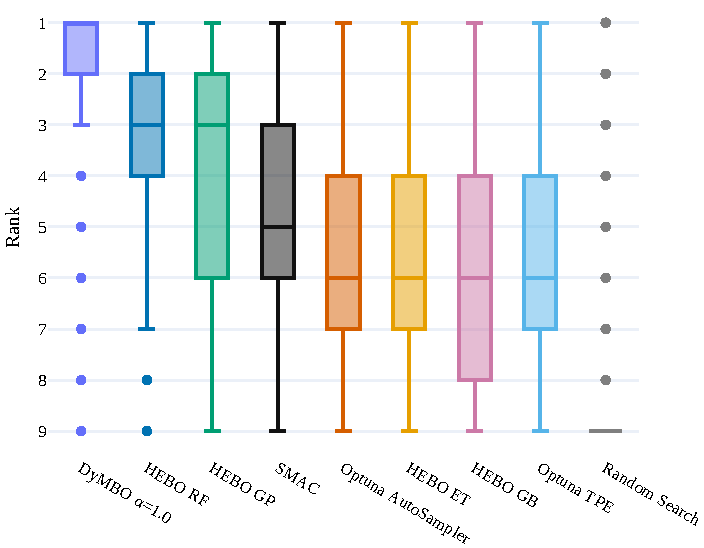
\includegraphics[width=0.5\linewidth]{figures/05/figs/figs/ranks/main_ranks_intro_box_plot_rank.pdf}
    \caption{
    % \changed{
    Box plot showing the ranks of various methods across 859 benchmark functions from YAHPO Gym and JAHS-Bench-201. \texttt{DyMBO} outperforms all baselines.
    % }
    }
    \label{fig:ch05:box_plot_mean_rank}
\end{figure}

The remainder of this paper is organised as follows: in~\cref{sec:ch05:back-rw}, we define the HPO problem, describe how BO operates, and position our approach with respect to related work on dynamically adapting BO components and using ensembles for enhancing BO performance.~\cref{sec:ch05:method} introduces 
% the \texttt{DyMBO} methodology.
our methodology for
% \changed{
dynamic ensembling and selection
% }
of surrogate models. 
In~\cref{sec:ch05:experiments}, we provide the technical details on the experimental setup and describe the benchmarks and baselines chosen for our empirical analysis. We present results and critically discuss them in~\cref{sec:ch05:res}. Finally, in~\cref{sec:ch05:concl-fw}, we provide concluding remarks and outline directions for future research.








\section{Background and related work}
\label{sec:ch05:back-rw}

In this section, we define the HPO problem and describe the working mechanisms of the BO framework. 
We also cover related work on dynamic design choices related to the components of BO, as well as using ensembles in BO.

\subsection{Hyperparameter optimisation} Let $\mathcal{A}$ be a learning algorithm with $n$ hyperparameters, $\Lambda_{i}$ the domain of the $i$-th hyperparameter, and $\mathbf{\Lambda} = \Lambda_{1} \times \Lambda_{2} \times \dots \Lambda_{n}$ the overall hyperparameter configuration space. 
We denote a hyperparameter configuration by $\mathbf{\lambda} \in \mathbf{\Lambda}$, and the algorithm $\mathcal{A}$ with its hyperparameters instantiated to $\mathbf{\lambda}$ by $\mathcal{A}_{\mathbf{\lambda}}$.
Given a dataset $D$, the objective of HPO is to find a hyperparameter configuration $\mathbf{\lambda}^{*}$ that minimises the loss $\mathcal{L}$ of a model fitted by algorithm $\mathcal{A}$ with hyperparameters $\mathbf{\lambda}$ on training data ${D}_{train}$, and evaluated on validation data ${D}_{validate}$, for a given loss function $\mathcal{L}$, \emph{i.e.},
\begin{equation}
\label{eq:ch05:def-hpo}
\mathbf{\lambda}^{*} \in \argmin_{\mathbf{\lambda} \in \mathbf{\Lambda}} 
\mathcal{L}(\mathcal{A}_{\mathbf{\lambda}}, {D}_{train}, {D}_{validate}) = \argmin_{\mathbf{\lambda} \in \mathbf{\Lambda}} c(\mathbf{\lambda})
\end{equation}
Here, $c(\mathbf{\lambda})$ is a shorthand for the loss function when $\mathcal{A}_{\mathbf{\lambda}}$ and $D$ are fixed.
Note that $c(\mathbf{\lambda})$ is a black-box function, without a closed-form expression nor analytic gradient information.

\subsection{Bayesian optimisation} 
\label{sec:ch05:bac_bo}

Bayesian optimisation (BO)~\citep{Mockus12,Garnett23,Frazier18,Kushner62,Kushner64} is a family of surrogate-based algorithms for efficient global optimisation of black-box problems.
Typically, BO consists of three main components: an \emph{initial design}, \emph{i.e.}, in HPO, a set of candidate hyperparameter configurations $\boldsymbol{\lambda} = (\lambda^{(1)},\ldots, \lambda^{(r)})$ and their evaluations 
$c(\boldsymbol{\lambda}) = (c(\lambda^{(1)}),\ldots, c(\lambda^{(r)}))$; a \emph{surrogate model} (fitted to the 
% initial 
observations) that returns an approximation $\hat{c}(\mathbf{\lambda})$ of the unknown loss function $c(\mathbf{\lambda})$ while capturing the uncertainty in the prediction $\hat{\sigma}(\mathbf{\lambda})$ on unobserved points in the search space; and an \emph{acquisition function}, which is optimised to suggest candidate solutions to be evaluated next, usually balancing exploration and exploitation of the search space.
BO then evaluates the most promising candidate solutions.
% \er{``interesting'' doesn't seem like a technical term. I would replace with ``promising'', ``valuable''...}
To approximate the expensive objective function, BO typically employs a Gaussian process (GP) model as the surrogate. The GP model defines a distribution over functions on the configuration space $c(\lambda)\sim\mathcal{GP}_c(\mu(\lambda),\text{cov}(\lambda,\lambda'))$, where 
$\mu(\cdot)$ 
is a mean function and 
$\text{cov}(\cdot,\cdot)$
is a covariance function. If we consider an observation model 
$y_i = c(\lambda^{(i)}) + \varepsilon_i$
with normally distributed noise, 
$\varepsilon_i\sim\mathcal{N}(0,\sigma^2_\varepsilon)$, 
the predicted value by the GP model at one unknown configuration 
$\lambda$ will also follow a normal distribution with mean 
$\mu(\lambda)=K_{\lambda,\boldsymbol{\lambda}}(K_{\boldsymbol{\lambda},\boldsymbol{\lambda}}+\sigma^2_\varepsilon I)^{-1}\boldsymbol{y}$ and variance $\sigma^2(\lambda)=\text{cov}(\lambda,\lambda)-K_{\lambda,\boldsymbol{\lambda}}(K_{\boldsymbol{\lambda},\boldsymbol{\lambda}}+\sigma^2_\varepsilon I)^{-1} K_{\boldsymbol{\lambda},\lambda}$, 
where $\boldsymbol{y}=(y_1,\ldots,y_r)$ is the vector of observations, $K_{\boldsymbol{\lambda},\boldsymbol{\lambda}}=[\text{cov}(\lambda^{(i)},\lambda^{(j)})]_{\lambda^{(i)},\lambda^{(j)}\in\boldsymbol{\lambda}}$ is the covariance matrix, and $K_{\lambda,\boldsymbol{\lambda}}=[\text{cov}(\lambda^{(i)},\lambda)]_{\lambda^{(i)}\in\boldsymbol{\lambda}}$ is the correlation vector for all samples.
% \aj{FIXED, please check: inconsistent use of bold for the lambda subscripts in the kernel K}
GPs as a surrogate model inherently provide both the mean and the variance vector.

However, GPs are not the only surrogate model used in BO. Another common choice for a surrogate model are tree-based models, 
such as random forests (RFs). 
Tree-based models traditionally predict only the mean of the given data (\emph{e.g.}, in a regression setting). 
In this case, the variance is defined based on the variance of the predictions of the leaves~\citep{HutEtAl11}. 
With $t(\lambda)$ being the prediction of a tree $t \in T$, we calculate the mean $\mu(\lambda)$ and variance $\sigma^2(\lambda)$ for a set of trees $T$ as follows:
% \hs{GB is now calculated as quantile regression}
\begin{equation}
    \mu(\lambda)=\frac{1}{|T|} \cdot \sum_{t\in T} t(\lambda) \; ,
\end{equation}
\begin{equation}
    \sigma^2(\lambda)=\frac{1}{|T|} \cdot \sum_{t\in T} (t(\lambda) - \mu(\lambda))^2 \; .
\end{equation}
% \changed{
% An exception is gradient boosting (GB), a tree-based model for which uncertainty is estimated via quantile regression~\citep{Koenker1978}.
% Here, two separate models are fitted to predict the upper and lower quantiles of the output distribution, and the variance is derived from the spread between these quantiles. This is done similarly to the implementation in the \textsc{scikit-optimize} package\footnote{\url{https://github.com/scikit-optimize/scikit-optimize}}.
% }
% \changed{
Alternatively, uncertainty can be estimated via quantile regression~\citep{KoeBas78}, using two separate models to predict the upper and lower quantile of the output distribution, and deriving variance from the spread between these quantiles.
We adopt this approach to estimate uncertainty for another tree-based model, gradient boosting (GB); this is done similarly to the implementation in the \textsc{scikit-optimize} package.\footnote{\url{https://github.com/scikit-optimize/scikit-optimize}}
% }
% \hh{this sounds as if the scikit-optimize implementation was the first to define GB ... surely not true?? please reword to properly reflect (a) the original concept of gradient boosting and (b) its implementation in the package. I'd also consider writing something like `Alternatively, uncertainty can be estimated as is done in gradient boosting, using two ... Footnote signs at the end of sentences follow the full stop.}

BO proceeds iteratively until a termination criterion is met. In each iteration, it optimises the acquisition function %to suggest high-potential solutions by
by repeatedly querying the surrogate model to generate a pool of candidate solutions. It then evaluates the most high-potential solutions (\emph{i.e.}, the solutions that maximise the acquisition function) from this pool,
refines the surrogate model based on the new observations, and updates the optimum if the new point improves upon the true function value of the best observation so far.
% \changed{
Throughout this work, we consider the batched setting, in which $k$ configurations are proposed and evaluated per BO iteration; see~\cref{sec:ch05:method}. This is reflected in the acquisition and update steps described here.
% }

Among the many variants of BO from the literature, in this work, we focus on the state-of-the-art method for HPO to empirically evaluate our method: HEBO~\citep{CowEtAl22}.
HEBO (Heteroscedastic and Evolutionary Bayesian optimisation) is a BO-based optimiser with several advancements 
% \changed{
targeting each of the core BO components described above.
For the surrogate model, HEBO uses GP with two key transformations: a power transformation applied to the output observations $\boldsymbol{y}$ and a Kumaraswamy transformation applied to the input configurations $\boldsymbol{\lambda}$; 
% \hh{minor change:}
jointly, these address heteroscedasticity in the noise $\epsilon$ and non-stationarity in the covariance matrix $K_{\boldsymbol{\lambda},\boldsymbol{\lambda}}$.
\citet{CowEtAl22} showed that these transformations enhance the ability of GPs to accurately approximate the mapping between configurations and corresponding performances, which is crucial for HPO.
% on performance data. 
% \er{``performance'' used twice with different meanings, could be confusing. What do we exactly mean with ``performance data'' and, earlier, with ``performance observations''? Is it another phrasing for solution quality, specific for HPO?}
For the acquisition function, rather than optimising a single criterion, HEBO samples new candidate configurations by maximising MACE~\citep{LyuEtAl18}, a multi-objective acquisition function that simultaneously considers expected improvement (EI)~\citep{Mockus75}, probability of improvement (PI)~\citep{Kushner64}, and upper confidence bound (UCB)~\citep{ForEtAl08}, providing a more robust balance between exploration and exploitation of the search space than any single acquisition function alone.
% \hh{modified:}
Additional details on HEBO can be found in~\cref{sec:imp_det}.

% \changed{
In conjunction with BO-based HPO techniques, \emph{multi-fidelity approaches}~\citep{LiEtAl18,LiEtAl20,FalEtAl18,AwaEtAl21} have been widely used to address expensive HPO problems, due to the fact that they use cheap approximations of the target function at hand.
However, these fall outside the scope of our work presented here, as they do not take into consideration the nature of the search space, but rather use low-fidelity evaluations as a proxy for full-fidelity evaluations to allow for the better use of the available budget; this constitutes a conceptually different approach from the one followed here.
% }
% }
% to improve performance. 
% \todo{connect the advancements of HEBO relative to the details of BO above to help understand where the gains of HEBO come from}
% It applies a power transformation to the performance data and 
% the Kumaraswamy transformation to the input data to tackle heteroscedasticity and non-stationarity. 






\subsection{Dynamic component selection in Bayesian optimisation}
As a modular framework, BO performance is highly sensitive to design choices of its modules. 
Different sampling strategies for the initial design, such as Latin hypercube sampling~\citep{McKEtAl00}, low-discrepancy sequences (\emph{e.g.}, Sobol~\citep{AntSal79}) or random uniform sampling; different surrogate models, such as GPs or RFs; and different acquisition functions, such as EI, PI or UCB -- all affect the overall BO performance to various degrees~\citep{BosEtAl20,LinEtAl19,CowEtAl22}. 
Despite few works showing the potential of automated selection of components~\citep{BenTom18,BenEtAl22,BenEtAl22}, the settings for each component are typically chosen by practitioners beforehand depending on the desired use-case, and are fixed for the entire optimisation procedure.

However, there have been efforts to show that the dynamic choices of BO modules lead to performance gains across multiple contexts.
Prior attempts to investigate the dynamic adjustment of acquisition functions include works on mixed acquisition function strategies, \emph{e.g.}, a self-adjusting approach to balance the exploration-exploitation trade-off~\citep{BenEtAl23}, an online multi-armed bandit strategy on a portfolio of acquisition functions~\citep{HofEtAl11}, or an online update of weights in a portfolio of acquisition functions~\citep{KanEtAl20}.
When it comes to dynamic adjustment of surrogate models, several directions have been investigated, notably an online selection of surrogate models based on their ranking in each BO iteration~\citep{BagEtAl16}, adaptive global surrogate modelling via genetic algorithm-driven sampling~\citep{GorEtAl09}, or adaptive combining of surrogates based on crowding distance trust regions~\citep{ZhaEtAl12}.
It has also been shown that dynamic component selection in general is beneficial in terms of performance in other related areas, \emph{e.g.}, in algorithm configuration~\citep{BieEtAl20}, evolutionary computation~\citep{KarEtAl15,DoeDoe20}, planning~\citep{SpeEtAl21}, and deep learning~\citep{AdrEtAl22}.

\subsection{Ensembles in Bayesian optimisation}
% \hs{clarify how we are different and novel}
% \changed{
Ensembles of ML models have been shown to outperform single models for a wide range of use-cases~\citep{SagRok18,OpiMac99,Rokach10,DonEtAl20}. 
Consequently, using ensembles in the context of BO is not a new idea.
% \changed{
Nevertheless, to the best of our knowledge, our work is the first one to use a 
% \hh{simplify: is the first to use a ...}
dynamic tailoring strategy, ranging from full ensembling to greedy selection, for surrogate models in mixed discrete-continuous search spaces of problems that tend to be very expensive to evaluate in practice, such as HPO.
% }
A series of earlier studies has demonstrated the advantage of using ensembles in BO, most notably in engineering~\citep{JiaEtAl20,ZhoEtAl11}; however, the search spaces explored in these are of a purely continuous nature.
Various ensembling strategies investigated in the literature do not apply in a straightforward manner to our use-case, \emph{e.g.}, optimal weighting strategies of surrogates trained on existing observations~\citep{HanEtAl22} or on extracted features~\citep{GuoEtAl19} have been designed for multi-objective constrained optimisation, while techniques for optimising multiple acquisition functions on multiple surrogates and combining them accordingly~\citep{HuaEtAl22, BeaEtAl19} have been developed for purely discrete search spaces.
Moreover, all these existing approaches consider a static (\emph{i.e.}, global) ensemble construction which is then used throughout the entire optimisation process. Additionally, ensembles of surrogate models are commonly used in meta-learning for BO~\citep{WisEtAl16,FeuEtAl22}. 
% \er{We use both BO and the full name, Bayesian optimization, in text. We should stick to BO once the acronym is introduced.}
% \aj{This is now fixed. We only use the full name ``Bayesian optimisation'' in the abstract, for the first time we introduce it in the manuscript, and then in section titles (because it is cleaner than using an acronym in the title, IMO, but we can change this), and in the Figure 1 caption, because it should be self-contained (but we can also change this). }
% \changed{
In contrast, our method operates in a dynamic fashion, tracking the accuracy of surrogates and adjusting the surrogate weighting on the fly.
% }

Dynamic model ensembles in BO have been used for time-series prediction~\citep{Liu23}, which constitutes a fundamentally different use-case. 
% \citet{Liu2020} have proposed a multi-fidelity approach by combining two GP %regression 
% models approximating both high- and low-fidelity data during the BO procedure, whereas our work considers a fully black-box setting. 
Dynamic ensembling has also been considered in a non-BO context, \emph{e.g.}, for neural decoding in brain-computer interfaces~\citep{QiEtAl19}.
% \hh{The next sentence needs to be modified, since it doesn't make an argument why these are incompatible (you could refer to what was stated earlier, of course).}
The fact that HPO problems can be expensive to evaluate and involve mixed discrete-continuous search spaces, with possibly many conditional hyperparameters, renders previous approaches hardly applicable in this context.
% The incompatibility of these works with the HPO use-case renders them non-applicable in our context.
Related approaches also substantially differ from our proposed methodology, as none of them considers the use of exponential moving averages to capture the history of model performance, nor a weighting scheme that is based on the accuracy on all past observations.
Furthermore, we consider ensembles of regression models from inherently different families.
% To the best of our knowledge, dynamic surrogate ensembles have so far not been applied in the context of HPO.
Thus, in relation to previous work, we not only consider a new use-case, but an entirely different challenge compared to other real-world applications, due to a key trade-off between the budget for evaluating the (possibly very expensive) target function and the budget for finding the optimal %hyperparameter 
configuration.
% }



\section{Methodology}
\label{sec:ch05:method}

% Our dynamic ensembling approach works as follows. 
% \changed{
Our method works as follows.
% }
The BO procedure is launched with an initial set of hyperparameter configurations. We initialise the weights and assign them to the models used to construct the ensemble. We denote the initial weight for the surrogate model $m$ as $w_{0,m}$. 
Then, the BO loop begins. At each iteration $t$, we train all surrogate models separately on all available samples accumulated up to that point and create a weighted ensemble. The weighted ensemble is a convex combination of the surrogate models, with coefficients defined as the normalised model weights of that iteration, \emph{i.e.},:
\begin{equation}
    \hat{w}_{t,m} = \frac{\bar{w}_{t,m}}{\sum_{j\in M}{\bar{w}_{t, j}}},
\end{equation}
where $M$ is the set of available surrogate models and $\bar{w}_{t,m}$ is the weight of model $m$ at iteration $t$. This way we make sure that $\sum_{m\in M} \hat{w}_{t,m} = 1$ with $0\leq \hat{w}_{t,m} \leq 1$.
The ensemble can then predict the $\mu_{\text{ens}}(\lambda)$ and $\sigma_{\text{ens}}(\lambda)$ of the performance for an unobserved configuration $\lambda$ by using a weighted average 
of the individual model predictions $\mu_m(\lambda)$ and their standard deviations $\sigma_m(\lambda)$:
\begin{equation}
    \mu_{\text{ens}}(\lambda)= \sum_{m\in M} \hat{w}_{t,m} \cdot \mu_{m}(\lambda),
    \label{ch05:ens_mu}
\end{equation}
\begin{equation}
    \sigma_{\text{ens}}(\lambda)= \sum_{m\in M} \hat{w}_{t,m} \cdot \sigma_{m}(\lambda).
    \label{ch05:ens_sigma}
\end{equation}

% \changed{
We note that~\cref{ch05:ens_sigma} combines the standard deviations $\sigma_{m}(\lambda)$ directly rather than the variances $\sigma_{m}^{2}(\lambda)$; we adopt this convention for consistency with the expected use of $\sigma_{ens}$ as a scale parameter in the acquisition function definition.
We discuss an alternative formulation based on the rule of total variance in~\cref{sec:ch05:ablations}.
% }
We also note that, in preliminary experiments, we investigated a variation of our ensembling method that applies different weighting schemes for the mean and the variance. However, this did not yield sufficient improvements to justify a more complex method definition. Further details can be found in~\cref{sec:ch05:ablations}.

% \hh{minor change in the following:}
% \changed{
\paragraph{Accuracy evaluation via ranking loss.}
In the next stages, at each iteration $t$, we optimise the acquisition function and select the candidates to be sampled, $\lambda_t^{(1)},\lambda_t^{(2)},\dots,\lambda_t^{{(k)}}$, as is typically done in BO. We then evaluate the accuracy of the different surrogate models using ranking loss (RL)~\citep{FeuEtAl22} on all sampled points. 
% \todo{ranking score/metric/weight instead of ranking loss since we do not use it as a loss function and there is no meta-learning... what do you think?}
% \aj{FIXED, added acronym RL in the sentence}
% \changed{
We use ranking loss as a model performance metric 
% \hh{I'd cut `indicator'; performance metric is a standard term.}
rather than as a loss function, as originally introduced by~\citet{WisEtAl16}, and we define it as:
% }
%\er{I am not sure we introduced all the symbols in Eq. (7) at this point. Did we define $\boldsymbol{C}$ as the sample set? I added the definition after the equation, please check. Also... I am not sure we should use subscripts to denote different samples, as we used it in the pseudocode to denote the iteration. Should we switch to the superscript in brackets for both $\lambda$ and $c$?}

    % \aj{Elena's comment: mathbb{1} compiles incorrectly} \er{Fixed. And changed the equation to be on one line.}
\begin{equation}
\label{eq:ch05:rl}
    \begin{aligned}
       \text{RL}(\mu_m, \boldsymbol{\lambda}) = 
        \sum_{\lambda^{(j)}\in \boldsymbol{\lambda}} 
        \sum_{\lambda^{(k)}\in \boldsymbol{\lambda}} 
        {1\kern-0.25em\text{l}}\big(
        &(\mu_m(\lambda^{(j)}) < \mu_m(\lambda^{(k)})) \\
        &\oplus (c(\lambda^{(j)}) < c(\lambda^{(k)}))
        \big).
    \end{aligned}
\end{equation}
% \todo{cross-validation not used, elaborate}
Ranking loss captures the number of incorrectly ranked pairs, \emph{i.e.,} the changes in the relative ordering of the predictions of the surrogate model compared to the true function values, given a pair of samples $(\lambda^{(j)},\lambda^{(k)})$ belonging to the sample set $\boldsymbol{\lambda}$ accumulated up to that point.

In particular for our optimisation use-case, ranking loss is more appropriate than other common choices of metrics for model performance, \emph{e.g.,} mean squared error (MSE). 
We do not seek the most accurate model in terms of predictive power; instead, we are interested in finding the location of the optimum. 
Therefore, the rank of the candidate solutions is more important than their specific values. 
% \hs{??}
% \changed{
% This is why we do not compute RL using cross-validation or a held-out set.
We use ranking loss to determine how well each surrogate ranks the points in $\boldsymbol{\lambda}$, which is directly observable without any held-out set. 
We provide an ablation for using a holdout set in~\cref{sec:ch05:ablations}.
% }
Additional results on the performance of our method in terms of MSE are also provided in~\cref{sec:ch05:ablations}.
% }

% \aj{in the following + in pseudocode, swapped w and w bar to be more intuitive (Reviewer 3)}
\paragraph{Weight update via exponential moving average.}
Based on the calculated ranking loss, we determine the new weights 
% \changed{
${w}_m$ 
% }
for each model greedily as follows:
% \todo{explain this as ''hard greedy weighting"}

% \aj{Elena's comment: why newline?} \er{Fixed it.}
% \changed{
\begin{equation}\label{eqn:ch05:weight}
    {w}_{t,m} =
    \begin{cases}
        1, & \text{if } \text{RL}(\mu_{t,m}, \boldsymbol{\lambda}) = \text{min}_{l \in M} \text{RL}(\mu_{t,l}, \boldsymbol{\lambda}), \\
        0, & \text{otherwise}.
    \end{cases}
\end{equation}
% }
% \er{Do I remember well that we found out with the extra experiments that our method works better when we evaluate the model accuracy on the entire history rather than on the points sampled in the last iteration only? If so, the formula above still says that we only compute the weights based on the points evaluated at iter $t$.}
%
% \er{$\text{RL}(\mu_{m}(\lambda_t),c(\lambda_t))$ incongruent notation with Eq. (7) for the first input argument.}
% where
% $
%     \lambda_t=\{\lambda_t^{(1)}, \lambda_t^{(2)}, \dots, \lambda_t^{(k)}\}.
% $
Therefore, in~\cref{eqn:ch05:weight}, 
we assign a weight of ${w}_{t,m} = 1$ to the model
% \hh{minor change:} 
with the lowest ranking loss on all points sampled up to iteration $t$.

% $k$
% new points $\lambda_t$
% sampled at iteration $t$. 
Then, for each model $m$, we use an exponential moving average between the previously calculated weights and the new weight:
% \changed{
\begin{equation}
    \bar{w}_{t+1,m} = (1-\alpha) \cdot \bar{w}_{t, m} + \alpha  \cdot {w}_{t,m} \; .
    \label{eq:ch05:weight_ema}
\end{equation}
% }
% \changed{
We use the exponential moving average in the weighting scheme so that the accumulated weight history, and not only the most recent model accuracy, determines the influence of each surrogate.
A surrogate that has been consistently accurate can therefore retain meaningful weight even at an iteration where it is not the single top performer under~\cref{eqn:ch05:weight}. We retain the term ``ensemble'' throughout to describe this general weighting mechanism, even though the special case when $\alpha = 1$ discards the history and becomes single-surrogate selection at each iteration.
% We use ``dynamic tailoring'' when referring to the mechanism spanning both ensembling and selection regimes.
% }

% \changed{
The smoothing factor $\alpha \in [0,1]$ governs how much of the newly assigned greedy weight ${w}_{t,m}$ is carried into the updated weight $\bar{w}_{t+1,m}$, relative to the weight already accumulated at iteration $t$. 
As $\alpha \to 0$, the update 
%\hh{cut one of the two:} \er{I like that both extreme cases are explained, especially since some reviewers have dismissed the method as mere selection. Perhaps this part could just be shortened a bit.}
progressively increasingly 
disregards the ranking loss of the current iteration and instead preserves the previously accumulated weights; in the limit, the ensemble composition stops reacting to which surrogate is currently most accurate, therefore becoming effectively static. 
In contrast, when $\alpha = 1$,~\cref{eq:ch05:weight_ema} collapses to $\bar{w}_{t+1,m} = {w}_{t,m}$, meaning that all weight history is discarded at every iteration, and the ensemble reduces to a selection of the single surrogate with the best ranking loss on all points sampled up to iteration $t$ (see~\cref{eqn:ch05:weight}).
Note that even at $\alpha = 1$, the method is not ``memoryless'' in the sense of ignoring past observations, as the ranking loss in~\cref{eq:ch05:rl} is itself computed cumulatively over the full sample set $\boldsymbol{\lambda}$ accumulated so far (including the initial design), rather than merely over the most recent batch. 
Therefore, $\alpha$ governs how quickly the method revises its belief about which surrogates currently deserve influence, and not whether past observations inform the weighting. 
% since they always do via ranking loss.
% }

% \changed{
Intermediate values of $\alpha$ are intended to mitigate two related failure modes. 
First, especially in early BO iterations, ranking loss is estimated from very few observations and can be noisy, so a surrogate may appear top-performing at a given iteration purely by chance.
In this case, an exponential moving average with $\alpha < 1$ dampens the effect of any single noisy update. 
Second, because different surrogate models tend to suit different regions of the search space, and the focus of the acquisition function narrows as optimisation proceeds, a surrogate that performed poorly during the more exploratory early phase may become preferable locally, near the optimum.
% In this case, retaining a fraction of its historical weight lets such a surrogate regain influence gradually, rather than requiring it to first ``win'' an iteration. 
% under~\autoref{eqn:weight}.
% Empirically, we find that the greedy end of this range, in particular $\alpha = 1$, performs best across the considered benchmarks considered (see~\autoref{fig:gen_res_simple}).
% We return to this finding, and to its relationship with surrogate ranking-loss quality and runtime, in Sections 5.4–5.6. We therefore treat $\alpha$ as a single, interpretable knob spanning a continuum from a near-static ensemble ($\alpha 0$) to greedy, per-iteration selection ($\alpha = 1$), rather than as evidence that one particular point on this continuum is uniquely correct; Section 5.3.6 and Appendix D show that the best-performing value shifts somewhat across benchmark families.
% }

% We use the exponential moving average in the weighting scheme to account for the history of the surrogate model performances, which is crucial for enabling the continual ensembling regime on top of greedy model selection at each iteration. 
% \aj{Something along the lines of: We retain the term ``ensemble'' throughout to describe the general weighting mechanism, even though the special case $\alpha$ = 1 reduces to a portfolio-style, single-model selection at each iteration; we use ``dynamic tailoring'' when referring to the general mechanism spanning both regimes.}
% \changed{
% With the exponential moving average, we ensure that the new greedily assigned weights are incorporated into the accumulated weight history, allowing for models that have been consistently good to retain meaningful influence even if they are not top performing at a particular iteration.
% Moreover, in the early stages of the BO procedure, the RL estimate can be noisy due to very few available observations, making it possible for a model to be top performing at a particular iteration by chance.
% This is addressed by the use of the exponential moving average by taking into account in each update the previous knowledge about the model performances.
% Last, different surrogate models may be better suited to different regions of the search space, and the acquisition function progressively focuses on a narrowing region as BO converges.
% A model that performed poorly in the global exploration phase may actually be top performing locally near the optimum.
% The exponential moving average allows such a model to accumulate weight gradually as optimisation progresses.
% }
% \todo{The following sentence needs more explanation and support as it is not clear what AFs were used in the baselines}

% \changed{
% \changed{
% The sample set $\boldsymbol{\lambda}$ over which we evaluate ranking loss contains all points observed so far in the optimisation process, including the initial design.
% Therefore, surrogate accuracy is assessed precisely at the regions of the search space the acquisition function currently favours, rather than uniformly across it.
% As the exploration-exploitation trade-off of the acquisition function shifts over the course of optimisation, the ranking-loss-based weighting tracks accuracy in the corresponding regions automatically (see~\autoref{eq:rl}), without requiring any additional mechanism.
% }
% We also want to respond to the exploration/exploitation tendency of the acquisition function, and therefore we accordingly reward the models that are accurate in the regions of the search space which are favoured by the acquisition function.
% \hh{slightly modified for language:}
We note that the acquisition function in HEBO trades off exploration and exploitation by combining EI, PI and UCB in a multi-objective way (for additional details, see \cref{sec:ch05:bac_bo,sec:ch05:ablations}).
We also provide details on acquisition functions used in different baselines in~\cref{sec:ch05:add_baselines}.
% }
% As we also want to respond to the exploration/exploitation tendency of the acquisition function, we accordingly reward the models that are accurate in the regions of the search space which are favoured by the acquisition function.

\paragraph{Pseudocode.}
We summarise our method in the pseudocode description provided in \cref{alg:ch05:debo}. \\
% \er{There numbering was incongruent with the new version of the pseudocode}
\noindent\textit{Initialisation (Lines 2--4). }
An initial set of $r$ hyperparameter configurations 
$\{\lambda_1,\ldots,\lambda_r\}$ is generated based on the sampling scheme of the chosen BO framework and then evaluated. The weights $w_{0,m}$ defining the model ensemble are also initialised. The iterative phase of BO starts and runs until the budget is exhausted.\\
\noindent\textit{Model fitting (Lines 6--7).} 
All models used to construct the ensemble are fitted to the data. Then, the model ensemble is computed as a weighted average of the single models.\\ 
\noindent\textit{Augment dataset with new points (Lines 8--10). }
The acquisition function $AF$ of the chosen BO framework
is optimised 
on the model defined by $(\mu_\text{ens},\sigma_\text{ens})$
to generate $k$ new solution candidates to improve the current best solution. 
The target function is evaluated on the new candidates, and the problem dataset is augmented with these new points.\\
\noindent\textit{Update weights (Lines 11--12).}
New model weights are computed based on the accuracy of the single models evaluated on all sampled solutions and weight history.\\
\noindent\textit{Return best configuration (Line 14).}
The best found %hyperparameter 
configuration $\lambda^*$ is returned as the optimal solution.

Note that, since our method is a plug-in for a generic BO framework, some of the steps (initial sample generation and acquisition function optimisation) depend on the specific BO framework.
% \changed{
We provide more details on these choices in~\cref{sec:imp_det}.
% }
% \changed{
% We note that \texttt{DyMBO} is designed to be a plug-in method that works well regardless of the chosen BO framework.
% Some of the steps (initial sample generation and acquisition function optimisation) are therefore inherited from the BO framework.
% We implement \texttt{DyMBO} in HEBO, and the initial design in HEBO is sampled via Sobol sequences.
% We employ the same Sobol sampling strategy for the single-surrogate baselines.
% For other HPO baselines, which are well-known methods that have been curated to achieve maximal performance, we use their own sampling strategy that in the past led to best performance, since we want to highlight that \texttt{DyMBO} outperforms other HPO methods ``at their best''. 
% }
% \todo{add info on initial design from the response letter here}

\begin{algorithm}
  \caption{\texttt{DyMBO:} Dynamic Complementary Surrogate Models in BO}
  
  \begin{algorithmic}[1]
        \STATE {\bfseries Input:} total budget $b$, size of newly sampled batch $k$, initial sample size $r$, loss function $c$, portfolio of surrogate models $M$, acquisition function $AF$, smoothing factor $\alpha$
        % \todo{AF is a portfolio (?) so (M, AF) should be input pairs; alpha should be a crucial input too}
        \STATE Initialise $\boldsymbol{\lambda}$ with $r$ randomly sampled points
        \STATE Evaluate initial samples: $\boldsymbol{C} \gets \{c(\lambda) \mid \lambda\in \boldsymbol{\lambda}\}$
        \STATE Initialise model weights $w_{0,m}$ 
        \WHILE{budget is not exhausted}
            \STATE Fit models to data: $\{(\mu_{m},\sigma_{m}) \mid m \in M\}\gets \{\text{fit}(m, \boldsymbol{\lambda}) \mid m\in M\}$
            \STATE Generate model ensemble $(\mu_\text{ens},\sigma_\text{ens})$ according to \cref{ch05:ens_mu,ch05:ens_sigma}
            \STATE Optimise acquisition function: $\lambda_t = \{\lambda_{t}^{(1)},\ldots,\lambda_t^{(k)}\}\gets \argmax AF(\lambda,\mu_\text{ens},\sigma_\text{ens},M)$
            % \todo{line 8, AF should take M as an input}
            \STATE Evaluate new candidates: $c_t = \{c_{t}^{(1)},\ldots,c_t^{(k)}\} \gets \{c(\lambda) \mid \lambda\in \lambda_t\}$
            \STATE Augment dataset: $\boldsymbol{\lambda} \gets \boldsymbol{\lambda} \cup \lambda_t$, $\mathbf{C} \gets \mathbf{C} \cup c_t$
            \STATE Calculate new model weights: ${w}_{t,m}$ according to \cref{eqn:ch05:weight}
            \STATE Update weights $\bar{w}_{t,m}$ according to \cref{eq:ch05:weight_ema}
        \ENDWHILE
        \STATE \textbf{Return} best configuration $\lambda^* \in \argmin_{\lambda \in \boldsymbol{\lambda}} \mathbf{C}$
  \end{algorithmic}
  \label{alg:ch05:debo}
\end{algorithm}







\section{Setup of experiments}
\label{sec:ch05:experiments}



We conducted a range of experiments to assess the performance of \texttt{DyMBO} in various HPO settings compared to a range of single-surrogate baselines and other competitive HPO frameworks.
In particular, we investigated how \texttt{DyMBO} performs in light of the trade-off between the time for evaluating the target function and the time for finding the optimal hyperparameter configuration.
We implemented our method in HEBO~\citep{CowEtAl22}, a state-of-the-art HPO framework~\citep{EggEtAl21}.
% \changed{
We provide implementation details and the description of the HEBO working mechanism in~\cref{sec:imp_det}.
% }
% \er{I am not a fan of this explanation of how HEBO works in the experimental setup. I would rather see it at the end of Section 2.2 and jump directly to the following paragraph here. But I leave it to you.} \aj{done, pls check}
% HEBO is a BO-based optimiser with several advancements to improve performance. It applies a power transformation to the performance data and 
% the Kumaraswamy transformation to the input data to tackle heteroscedasticity and non-stationarity. 
% \citet{CowEtAl2022} 
% showed that these transformations improve the performance of Gaussian processes on performance data. 
% HEBO 
% samples new solution candidates by maximising the MACE~\citep{LyuEtAl18}, a multi-objective acquisition function that consists of EI, PI, and UCB~\citep{Forrester2008}. \er{removed the full name of UCB because already introduced}
% Since HEBO natively optimises a multi-objective acquisition function, we provide an ablation analysis for other common acquisition functions in~\autoref{sec:abl_af}.
%The acq finds new candidates using the multi-objective algorithm NSGA-II~\citep{}.

% \changed{
We considered two families of surrogate models to construct the ensemble: GPs and tree-based models.
From the latter, we selected three different models that have been widely used in the literature for approximating functions for the optimisation purposes, namely 
RF~\citep{Breiman01}, GB~\citep{Friedman01} and extremely randomised trees (ET)~\citep{GeuEtAl06}.
% random forest (RF)~\citep{Bre2001}, extremely randomised trees (ET)~\citep{GeuEtAl06} and gradient boosting (GB)~\citep{Friedman01}.
We considered all different combinations of these models within our method, with particular emphasis on the combination of GP and RF as the most prominent surrogate models for HPO, which was found to yield the best performance. 
% \er{What does ``particular emphasis'' mean here? Don't we also include GB and ET in the portfolio of surrogate models M?}
% \aj{this means that the results in the main body of the paper are based on the combination of GP and RF (so in all plots where we report DyMBO we use only GP and RF). The results where we include GB and ET are in Section 5.3.5.}
Details on the performance of all different surrogate model combinations are provided in~\cref{sec:ch05:ablations}.
% }
% \hh{This was incorrect; I've tried to fix it and also streamline the text. The old version commented out in the source.}
%\changed{We initialise the weights by assigning a weight of $1$ to RF ($w_{0,RF}=1$) and $0$ to GP ($w_{0,GP}=1$). An ablation for different initialisation strategies can be found in the Appendix~\ref{sec:init_ablation}.}
% \changed{
We initialised the weights by assigning  $w_{0,RF}=1$ for RF and $w_{0,GP}=0$ for GP. 
In~\cref{sec:ch05:ablations}, we also provide an ablation analysis for different initialisation strategies.
% }
% For GP, we used its native implementation from HEBO.
% For tree-based models, we used the \texttt{scikit-learn} implementation of RF, ET and GB.
% For details on these methods, refer to~\autoref{ssec:surrogates}.


% As GPs are preferable for scenarios with continuous hyperparameters and RFs better handle discrete (and even mixed and conditional) domains~\citep{EggEtAl2013}, we initialised the weights in the following manner: if the problem instance contains only continuous hyperparameters, we assign a weight of $1$ to Gaussian process ($w_{0,GP}=1$) and $0$ to all other surrogate models; otherwise, we assign a weight of $1$ to RF ($w_{0,RF}=1$) and $0$ to all other surrogate models.


% \changed{
% \changed{
We considered six values of the smoothing factor $\alpha$ of the exponential moving average for the dynamic tailoring mechanism,  $\alpha\in\{0.01,0.05,0.1,0.5,0.9,1.0\}$,
% The results of the corresponding ablation analysis can be found in~\autoref{sec:app_alpha}. 
% \aj{reference incorrect and not even needed, this is now part of the main results? I will remove this as soon as it is confirmed. But then those are not preliminary experiments, so I will make the changes accordingly}
% }
% The lower the $\alpha$, the lower the impact of the new weights in each iteration, \emph{i.e.}, the higher the impact of the history of the weights.
spanning dynamic ensembling regimes (when $\alpha$ is low) to pure selection (when $\alpha=1$ and no weight history is taken into account beyond the single most accurate surrogate).
% }
% In the latter case, we select only one model -- the one with the highest accuracy on all sampled points.
% \changed{
% The lower the $\alpha$, the lower the impact of the new weights in each iteration, \emph{i.e.}, the higher the impact of the history of the weights.
Thus, $\alpha$ controls the trade-off between responsiveness to the most recent weights and stability over the accumulated weight history.
% }
% -- rather than construct a weighted ensemble. 
% \er{Is this conclusion sentence necessary in the exp setup?} 
% \aj{we can move it to the results, but IMO it can also stay here, especially because for alpha = 1 we talk about shortest running time in the paragraph below. So we already talk about some conclusions...}
% We found that $\alpha=1$ exhibits the best overall performance, closely followed by $\alpha = 0.9$ as the target functions become more expensive.%, although no $\alpha$ value dominates.
% \todo{Could the authors please explain more about how having alpha = 0.9, already affects the algorithm optimization, when in fact, as the target function becomes more expensive, the BO iteration’s optimization cost can afford to be more costly?}
% \aj{I think the reviewer misunderstood the sentence above. We are reporting the overall performance of our method with alpha set to 0.9, not making observations re: evaluation vs optimisation cost at this stage. I would thus remove the sentence above from this section, as it talks about the results which can be seen from the plot -- mentioning it in the experimental setup is too early. Besides, we will add more fine-grained alpha values.}

In each iteration, the models with null weights are dynamically pruned, \emph{i.e.}, not considered at inference time. In the case of selection ($\alpha=1$), only the model achieving the highest accuracy on all sampled solutions is assigned a weight of $w=1$, while all other models receive $w=0$. 
% Thus, $\alpha=1$ performs model selection rather than ensembling, as no historical information is used. 
% The $\alpha=1$
The selection regime leads to the shortest running time, due to the fact that in acquisition function optimisation having fewer models with non-zero weights reduces inference time, since fewer models need to be accessed altogether.

We used the native implementations of the initial design sampling and the acquisition function in HEBO; an ablation study on different acquisitions can be found in~\cref{sec:ch05:ablations}.
We set the size of the initial sample to 8 for all experiments; results with different initial sample sizes can be found in~\cref{sec:ch05:diff_exp_setup}.
Each method ran with 51 different random seeds and with a total budget of $100 \times$ mean evaluation time, similarly to~\citet{EggEtAl21}. 
More details on the evaluation time are available in~\cref{sec:ch05:benchs}. %$\{0, \dots, 50\}$.


% \subsection{Benchmarks and baselines}
We empirically evaluated our approach on two benchmark suites, YAHPO Gym~\citep{PfiEtAl22} and JAHS-Bench-201~\citep{BanEtAl22}.
YAHPO Gym is a surrogate-based benchmark for hyperparameter optimisation, consisting of 15 scenarios (\emph{i.e.}, machine learning pipelines and their configuration space) on various datasets.
In particular, it contains LCBench~\citep{ZimEtAl21}, which is used to optimise neural networks on tabular data, and yields a purely numerical search space; combined algorithm selection and hyperparameter optimisation (CASH) on OpenML datasets~\citep{BinEtAl20,FalEtAl18}; as well as the NAS Bench 301~\citep{ZelEtAl22}. 
From YAHPO Gym, we used all 856 available instances.
JAHS-Bench-201 is a surrogate-based benchmark for optimisation of the architecture and hyperparameters of convolutional neural network on image datasets. 
From JAHS-Bench-201, we used all three available instances, each optimising the architecture for a different dataset.
% \changed{
Both YAHPO Gym and JAHS-Bench-201 contain mixed discrete-continuous search spaces. 
% }
For further experimental and implementation details, refer to~\cref{sec:imp_det,sec:ch05:benchs}.
% \changed{
For results on additional benchmarks, refer to~\cref{sec:ch05:add-bench}.
% }


% \changed{
We used single-surrogate BO variants within HEBO with each of the surrogate models considered (GP, RF, ET, and GB) as baselines to compare against \texttt{DyMBO}. 
Furthermore, we compared \texttt{DyMBO} to additional standard HPO methods: random search (RS)~\citep{BerEtAl11}, SMAC3~\citep{LinEtAl22, HutEtAl11}, Optuna with TPE as a surrogate model~\citep{BerEtAl11,AkiEtAl19}, and Optuna AutoSampler, which automatically selects HPO method based on hand-crafted rules~\citep{Ozaki24}.
More details on these baselines are provided in~\cref{sec:ch05:add_baselines}.
% }


% \subsection{Experimental protocol}

% \er{I am not sure about the difference between the content in the Experimental protocol subsection and the first part of the Experimental Setup section. But this might be just a matter of habits :)}
% \aj{if I remember correctly this was Holger's instruction, to have all technical details (how manu runs, what budget etc) in the "protocol" subsection}



\section{Results and discussion}
\label{sec:ch05:res}

In this section, we present and discuss the experimental results comparing \texttt{DyMBO} to the baselines. 
We first present the mean rank results on different benchmarks for various budgets in~\cref{sec:ch05:res_general}, whereas results under different experimental setups and ablation studies can be found in~\cref{sec:ch05:diff_exp_setup,sec:ch05:ablations}, respectively. We then analyse the running time required by our method in~\cref{sec:ch05:running_time}, discuss the evolution of the weights assigned to surrogate models throughout the optimisation process in~\cref{sec:ch05:weights}, and assess the predictive quality of the surrogate models used in the ensembles themselves in~\cref{sec:ch05:surr-acc}.
% We then analyse the evolution of the weights assigned to surrogate models throughout the optimisation process, and finally assess the running time of our method.

\subsection{Overall performance}
\label{sec:ch05:res_general}

% \begin{figure*}[h]
%     \centering
%     \begin{subfigure}[t]{0.49\textwidth}
%         \centering
%         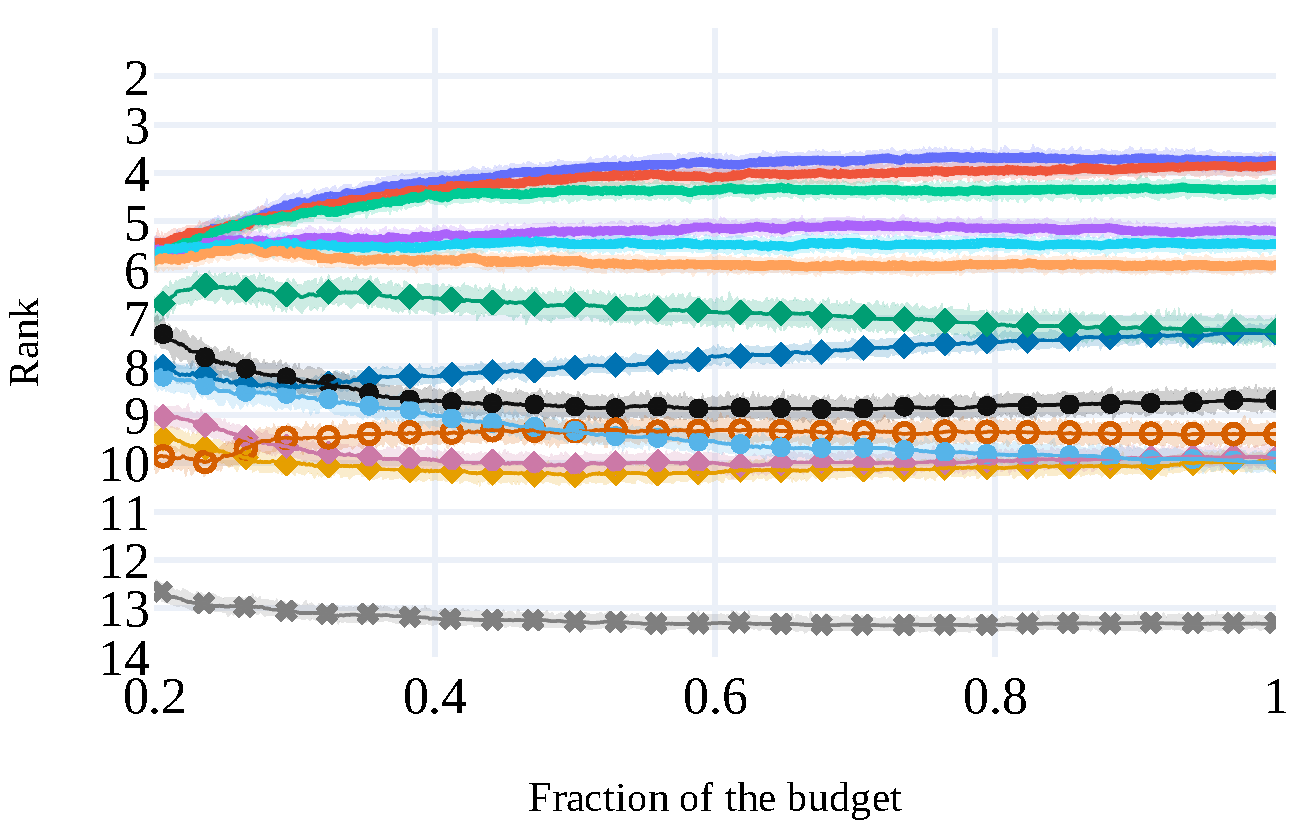
\includegraphics[scale=0.33]{figures/06/figs/figs/ranks/main_ranks_all.pdf}
%         \caption{All target functions}
%     \end{subfigure}
%     \begin{subfigure}[t]{0.49\textwidth}
%         \centering
%         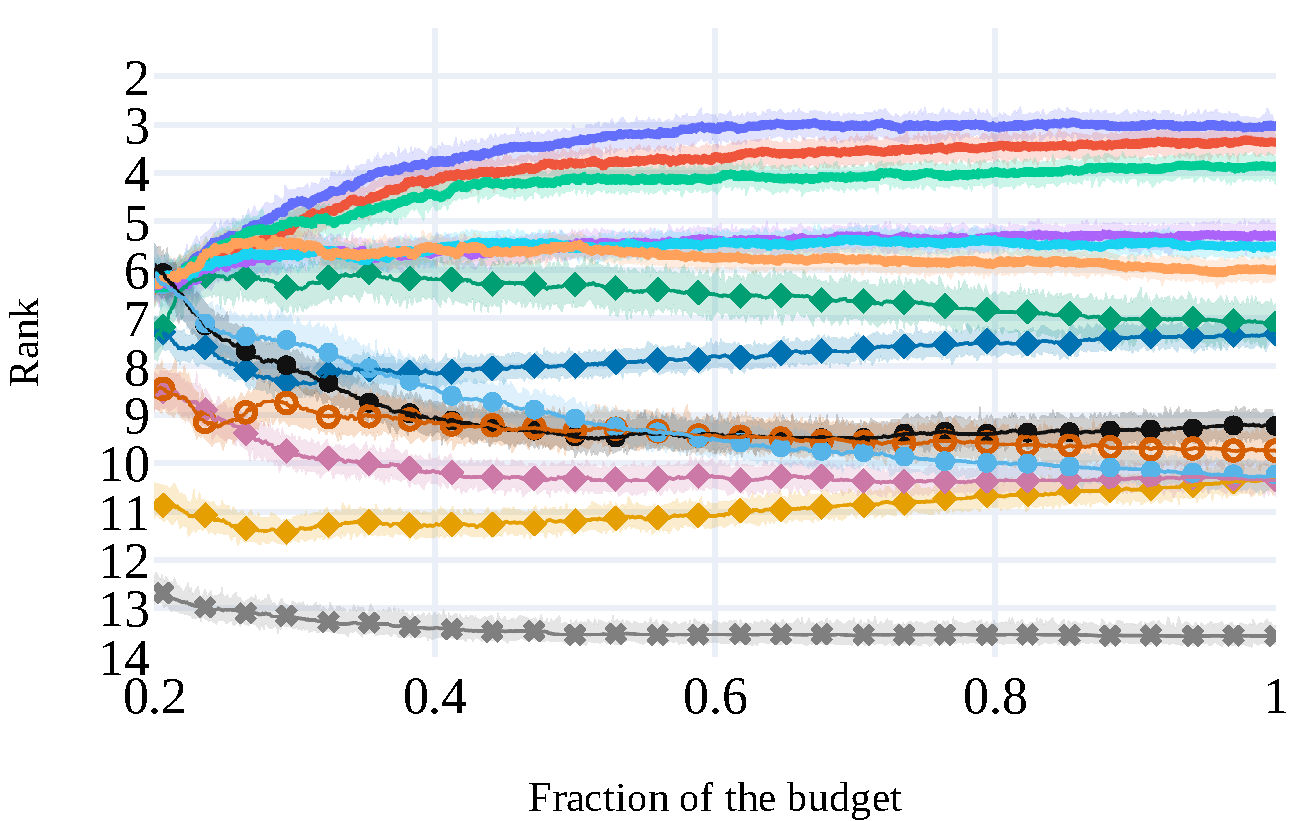
\includegraphics[scale=0.33]{figures/06/figs/figs/ranks/main_ranks_cheap.pdf}
%         \caption{Cheap (up to 10 minutes)}
%     \end{subfigure}
%     \begin{subfigure}[t]{0.49\textwidth}
%         \centering
%         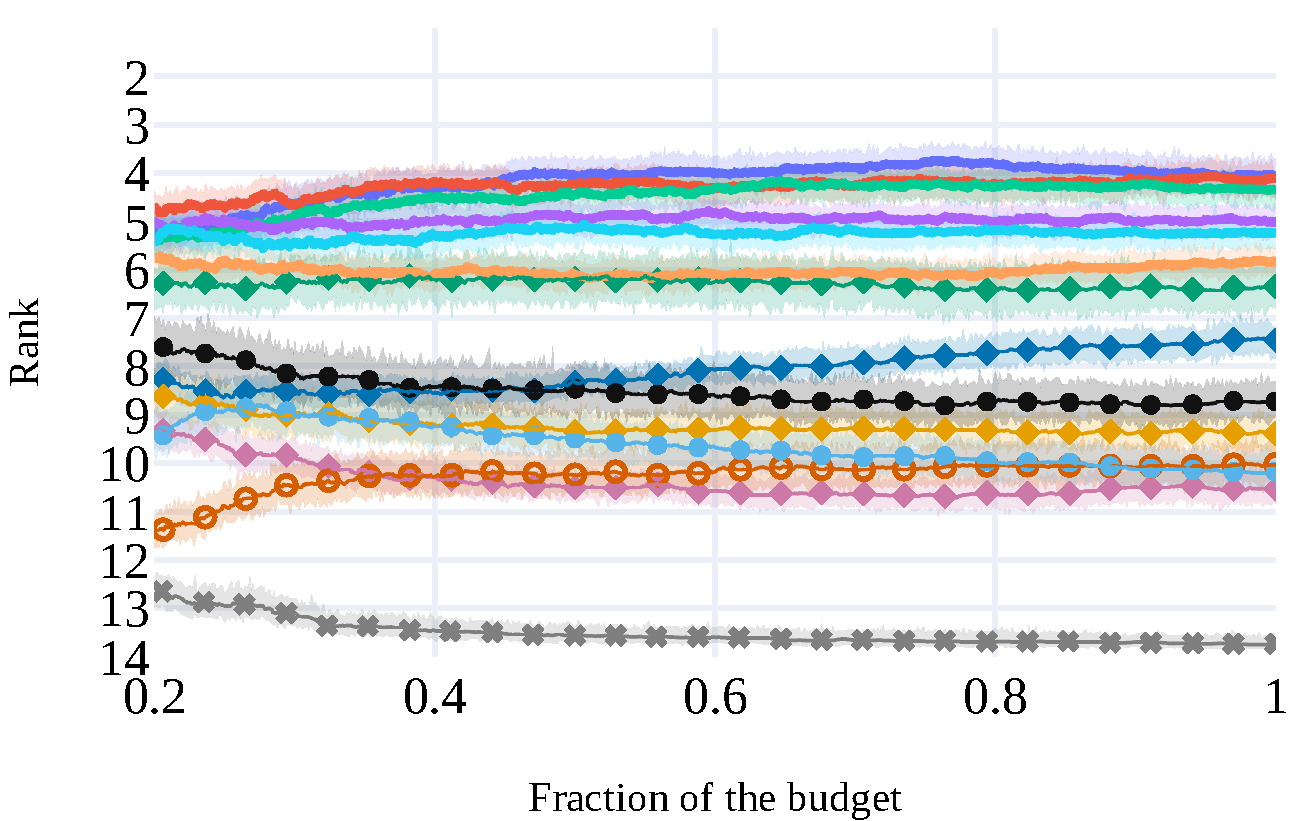
\includegraphics[scale=0.33]{figures/06/figs/figs/ranks/main_ranks_medium.pdf}
%         \caption{Medium-cost (more than 10 minutes, up to \mbox{1 hour})}
%     \end{subfigure}
%     \begin{subfigure}[t]{0.49\textwidth}
%         \centering
%         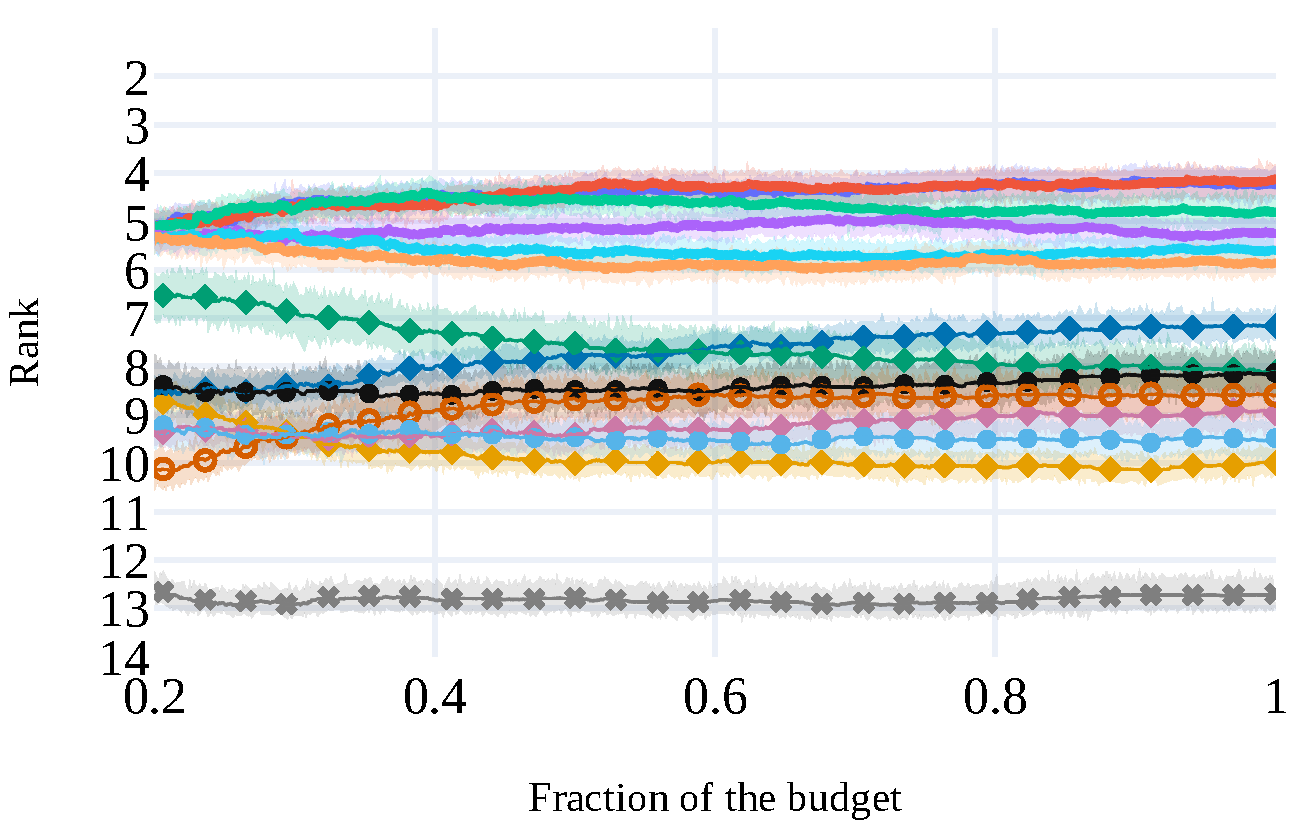
\includegraphics[scale=0.33]{figures/06/figs/figs/ranks/main_ranks_expensive.pdf}
%         \caption{Expensive (more than 1 hour)}
%     \end{subfigure}
%     \begin{subfigure}[t]{\textwidth}
%         \centering
%         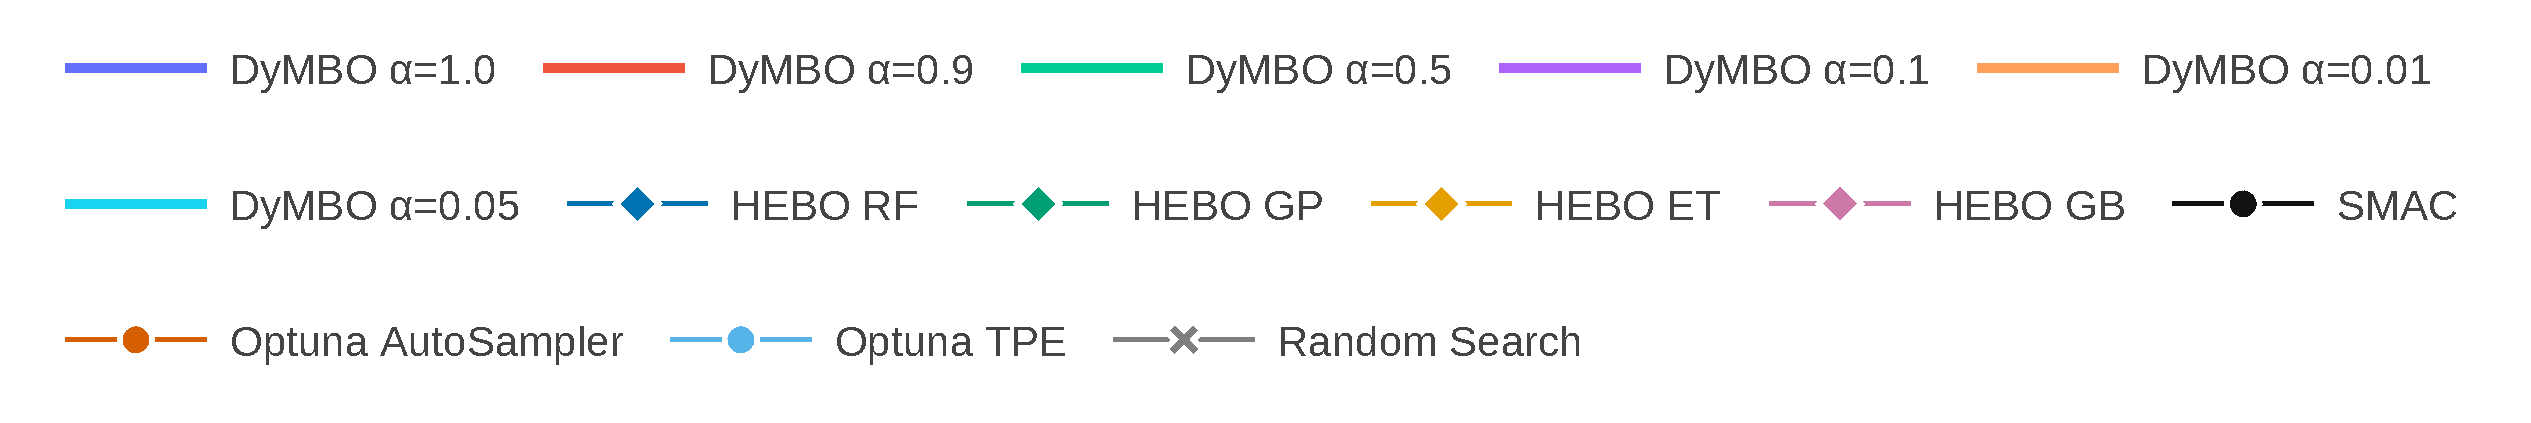
\includegraphics[scale=0.33]{figures/06/figs/figs/ranks/main_ranks_expensive_legend.pdf}
%     \end{subfigure}
%     \caption{
%     Mean ranks of \texttt{DyMBO} \changed{(with different values of $\alpha$)}, HEBO with different surrogate models, and other HPO methods on YAHPO Gym and JAHS-Bench-201, split according to different budgets: (a) all target functions, (b) cheap target functions with a budget of up to 10 minutes, (c) medium-cost target functions with a budget between 10 minutes and up to 1 hour, (d) expensive target functions with a budget of more than 1 hour. %\hh{slightly modified:}
%     % \changed{
%     Although different methods ranked differently with different target functions costs, \texttt{DyMBO} achieves the top rank across all target functions.%}
%     % \todo{Could the authors include some runs with alpha = \{0.01,0.05\}, especially for long budgets?}
%     % \hs{running}
%     % \todo{improvements: pull out the legends outside the plot and increase font size; aspect ratio to maximise usage of space with larger label fonts; colours not enough -- use markers, styles and opacity (worse algos = lower opacity); 4a) x-axis unclear -- make x-axis actual wall-clock time; choose a stronger subset of algos (especially with another BO baseline from the literature) and show primary results here, and show comprehensive results later}
%     }
%     \label{fig:gen_res}
% \end{figure*}



% \changed{
We begin by comparing \texttt{DyMBO} variants with different $\alpha$ values in~\cref{fig:ch05:gen_res_alpha}. We present the average rank as a function of the fraction of the budget for YAHPO Gym and JAHS-Bench-201. The results are split into four parts, according to the mean time required for evaluating the target function. Therefore, we show mean ranks on all target functions, on cheap functions with a budget of up to 10 minutes, on medium-cost functions with a budget
between 10 minutes up to 1 hour, and on expensive functions with a budget exceeding 1~hour. 
We observe that for cheap benchmarks, the selection variant ($\alpha=1.0$) works best, while the advantage of it compared to lower $\alpha$ values diminishes when the budget grows, whereas for expensive benchmarks, selection has similar performance to $\alpha=0.9$. Over all target functions, $\alpha=1.0$ works best.
% }


\begin{figure*}[h]
    \centering
    \begin{subfigure}[t]{0.49\textwidth}
        \centering
        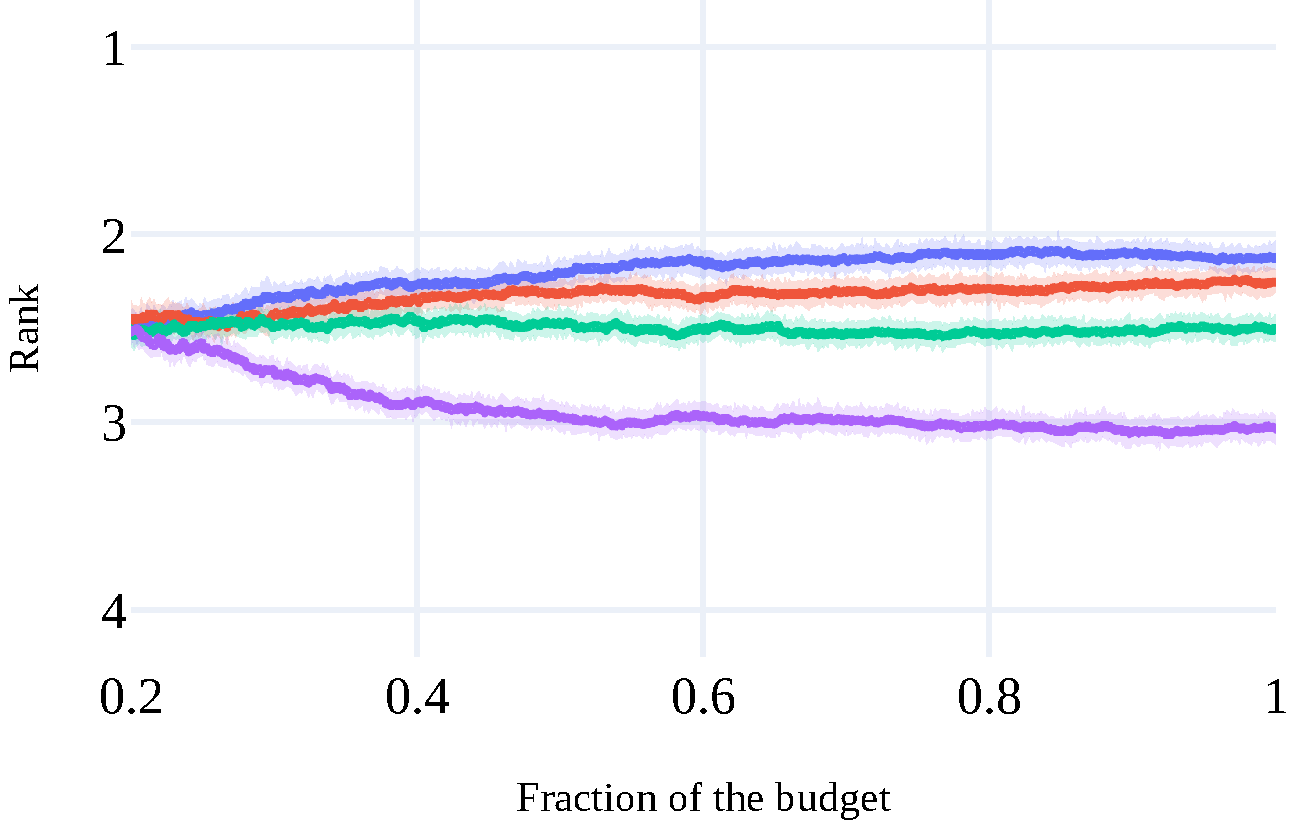
\includegraphics[scale=0.33]{figures/05/figs/figs/ranks/alpha_ablation_all.pdf}
        \caption{All target functions}
    \end{subfigure}
    \begin{subfigure}[t]{0.49\textwidth}
        \centering
        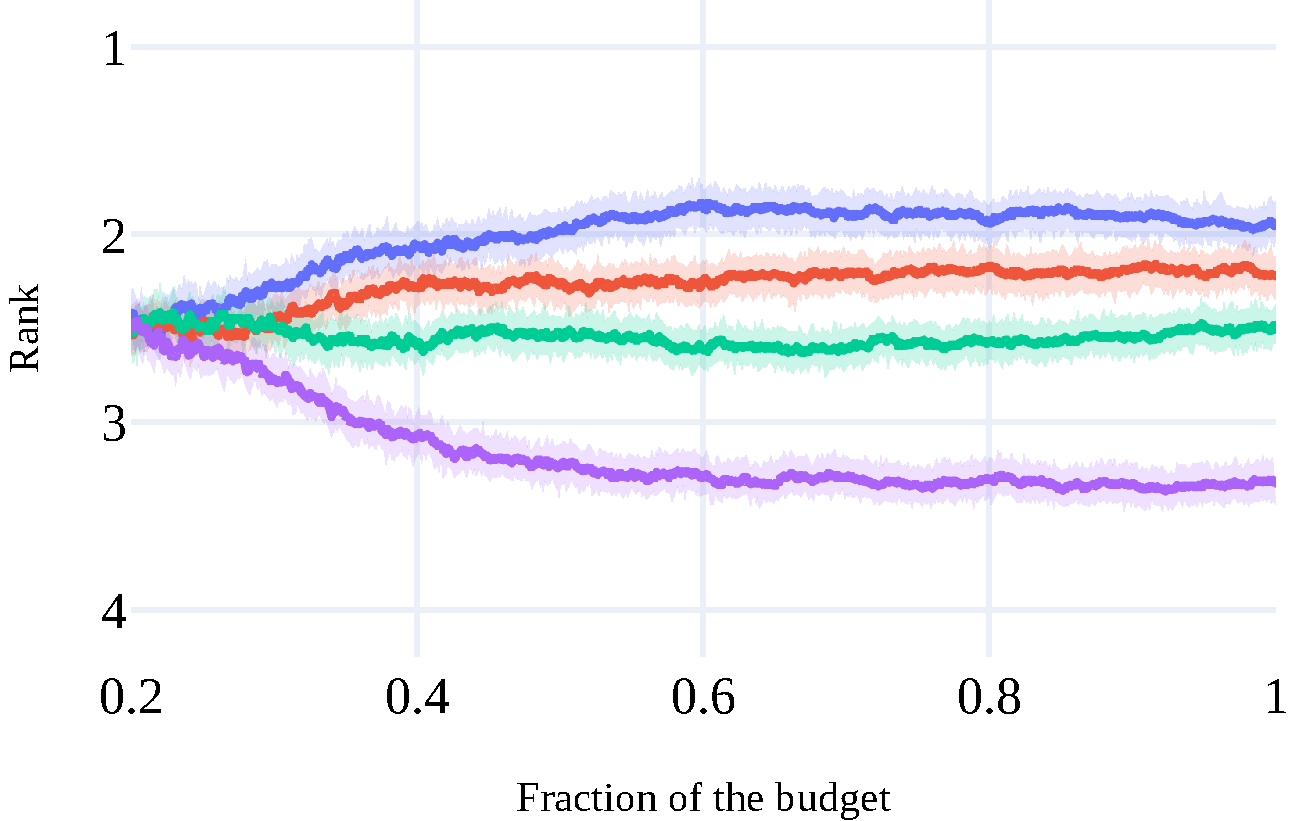
\includegraphics[scale=0.33]{figures/05/figs/figs/ranks/alpha_ablation_cheap.pdf}
        \caption{Cheap (up to 10 minutes)}
    \end{subfigure}
    \begin{subfigure}[t]{0.49\textwidth}
        \centering
        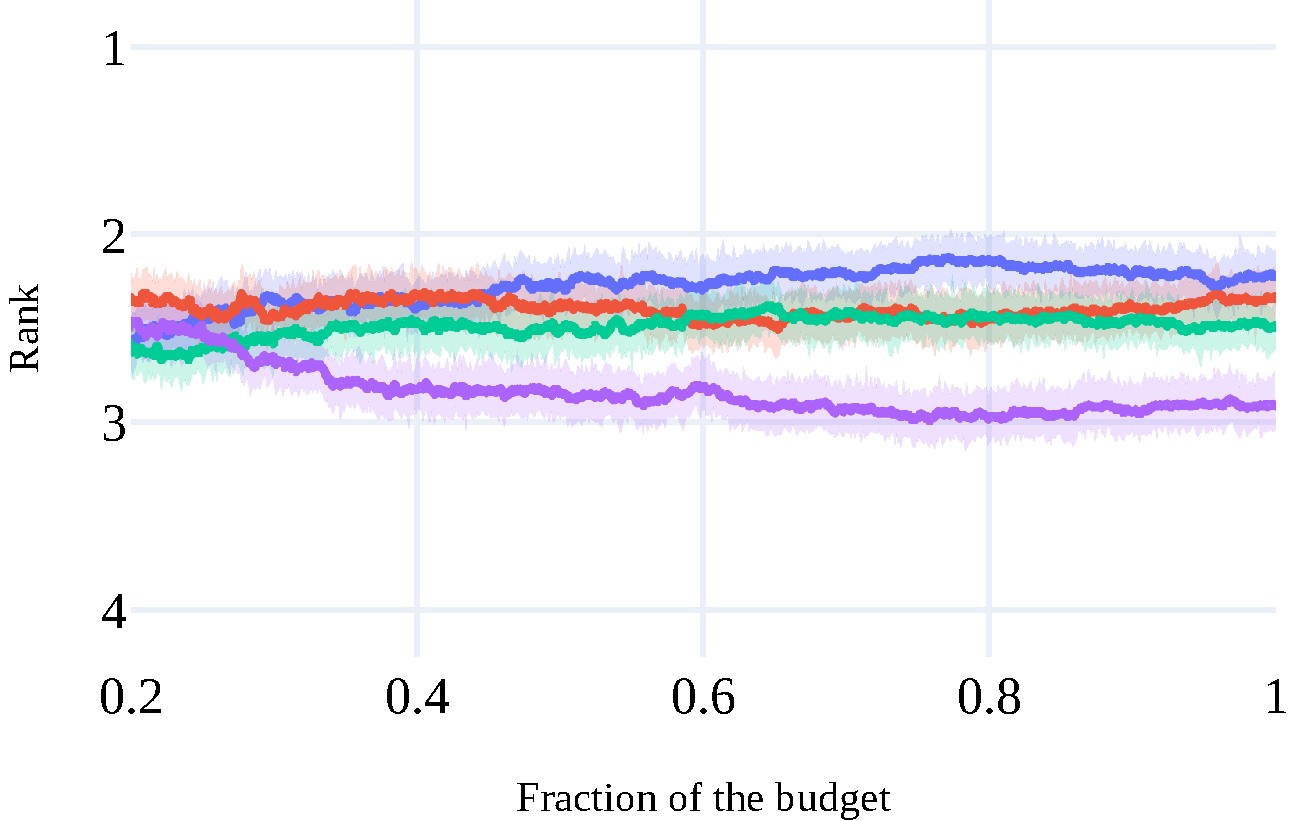
\includegraphics[scale=0.33]{figures/05/figs/figs/ranks/alpha_ablation_medium.pdf}
        \caption{Medium-cost (more than 10 minutes, up to \mbox{1 hour})}
    \end{subfigure}
    \begin{subfigure}[t]{0.49\textwidth}
        \centering
        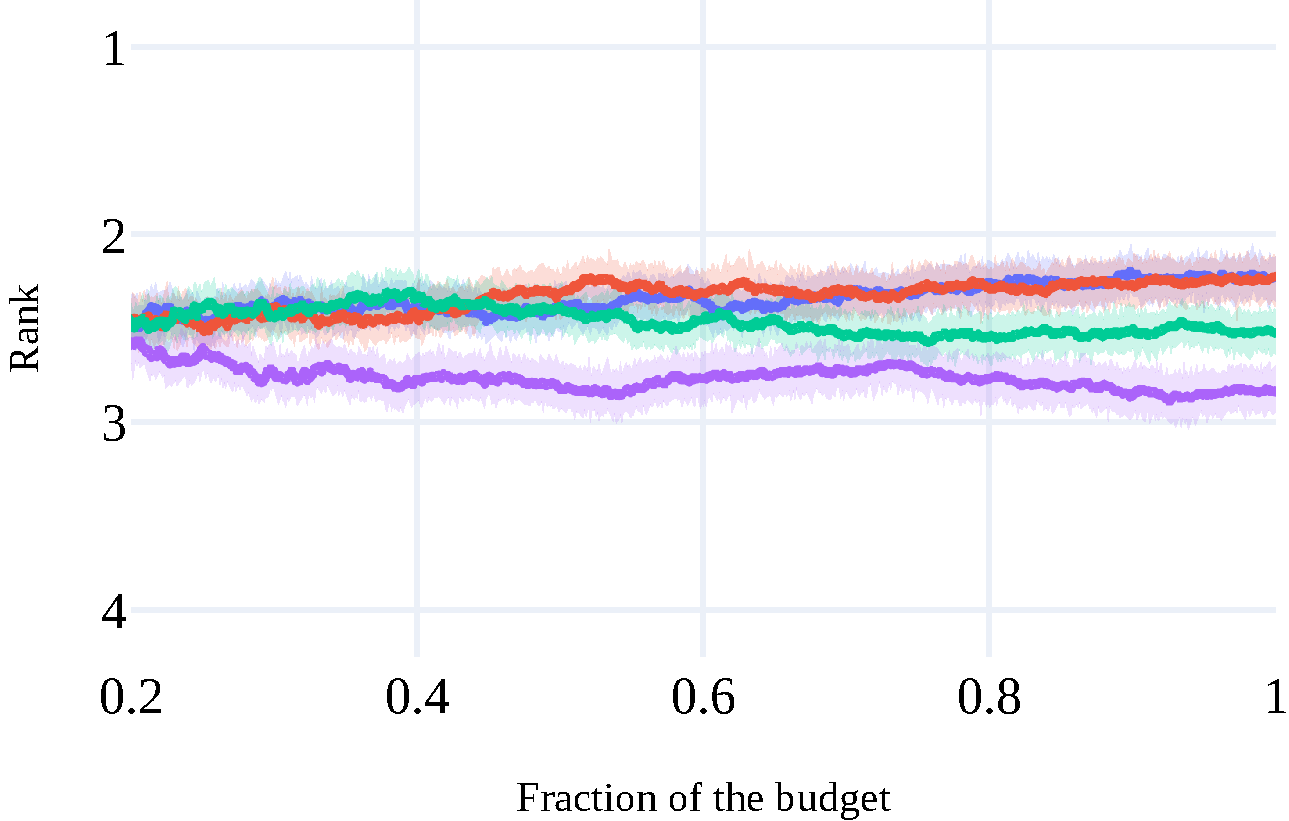
\includegraphics[scale=0.33]{figures/05/figs/figs/ranks/alpha_ablation_expensive.pdf}
        \caption{Expensive (more than 1 hour)}
    \end{subfigure}
    \begin{subfigure}[t]{\textwidth}
        \centering
        
\includegraphics[scale=0.33]{figures/05/figs/figs/ranks/alpha_ablation_all_legend.pdf}
    \end{subfigure}
    \caption{
    % \hs{
    Mean rank of \texttt{DyMBO} with ($\alpha \in {1.0, 0.9, 0.5, 0.1}$) on YAHPO Gym and JAHS-Bench-201 as a function of the fraction of the wall-clock time budget of each task. Results are shown for (a) all target functions, (b) cheap functions with budgets of up to 10 minutes, (c) medium-cost functions with budgets between 10 minutes and 1 hour, and (d) expensive functions with budgets exceeding 1 hour. Lower ranks indicate better performance. The greedy selection variant ($\alpha=1.0$) achieves the best overall mean rank, while its advantage decreases for more expensive target functions.
    % }
    }
    \label{fig:ch05:gen_res_alpha}
\end{figure*}

% \hs{
% We begin by comparing the different \texttt{DyMBO} variants with different $\alpha$ values in~\autoref{fig:gen_res_alpha}. We present the average rank as a function of the fraction of the budget for YAHPO Gym and JAHS-Bench-201. The results are split into four parts according to the mean time required for evaluating the target function. Therefore, we show mean ranks on all target functions, on cheap functions with a budget of up to 10 minutes, on medium-cost functions with a budget
% between 10 minutes up to 1 hour, and on expensive functions with a budget exceeding 1 hour. 
% We observed that for cheap benchmarks, $\alpha=1.0$, the selection variant works best, while the advantage of it compared to other $\alpha$ values diminishes when the budget grows, as for expensive benchmarks, it has similar performance to $\alpha=0.9$. Over all target functions, $\alpha=1.0$ works best.
% }
\begin{figure*}[h]
    \centering
    \begin{subfigure}[t]{0.49\textwidth}
        \centering
        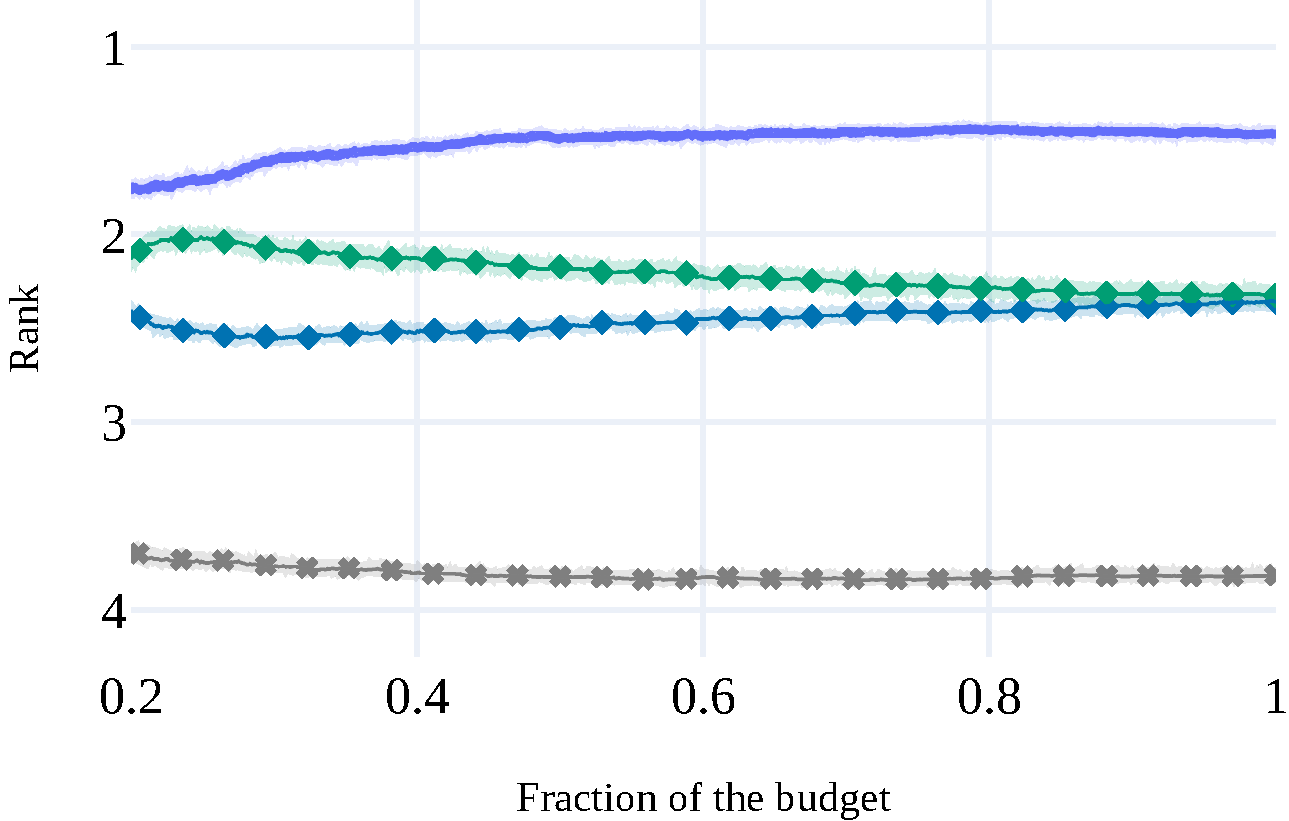
\includegraphics[scale=0.33]{figures/05/figs/figs/ranks/main_ranks_simple2_all.pdf}
        \caption{All target functions}
    \end{subfigure}
    \begin{subfigure}[t]{0.49\textwidth}
        \centering
        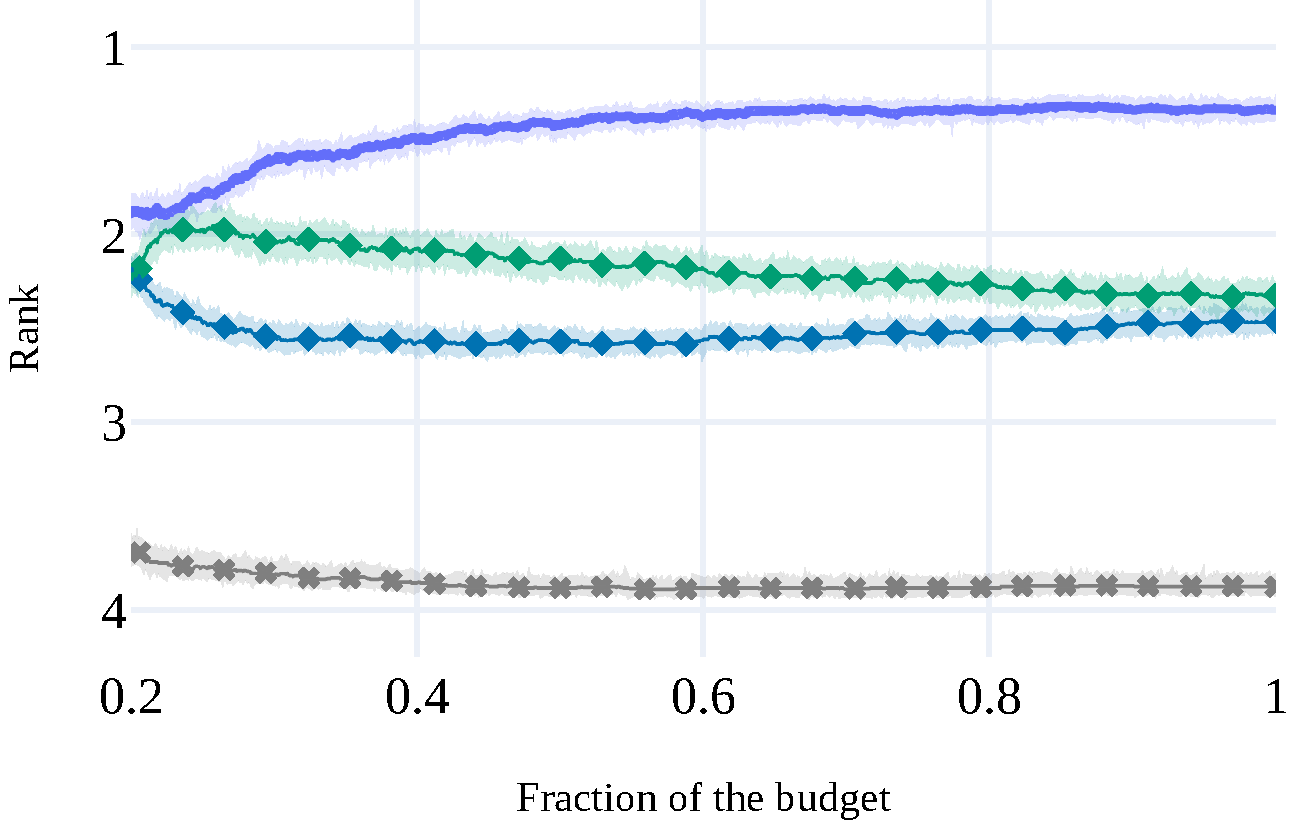
\includegraphics[scale=0.33]{figures/05/figs/figs/ranks/main_ranks_simple2_cheap.pdf}
        \caption{Cheap (up to 10 minutes)}
    \end{subfigure}
    \begin{subfigure}[t]{0.49\textwidth}
        \centering
        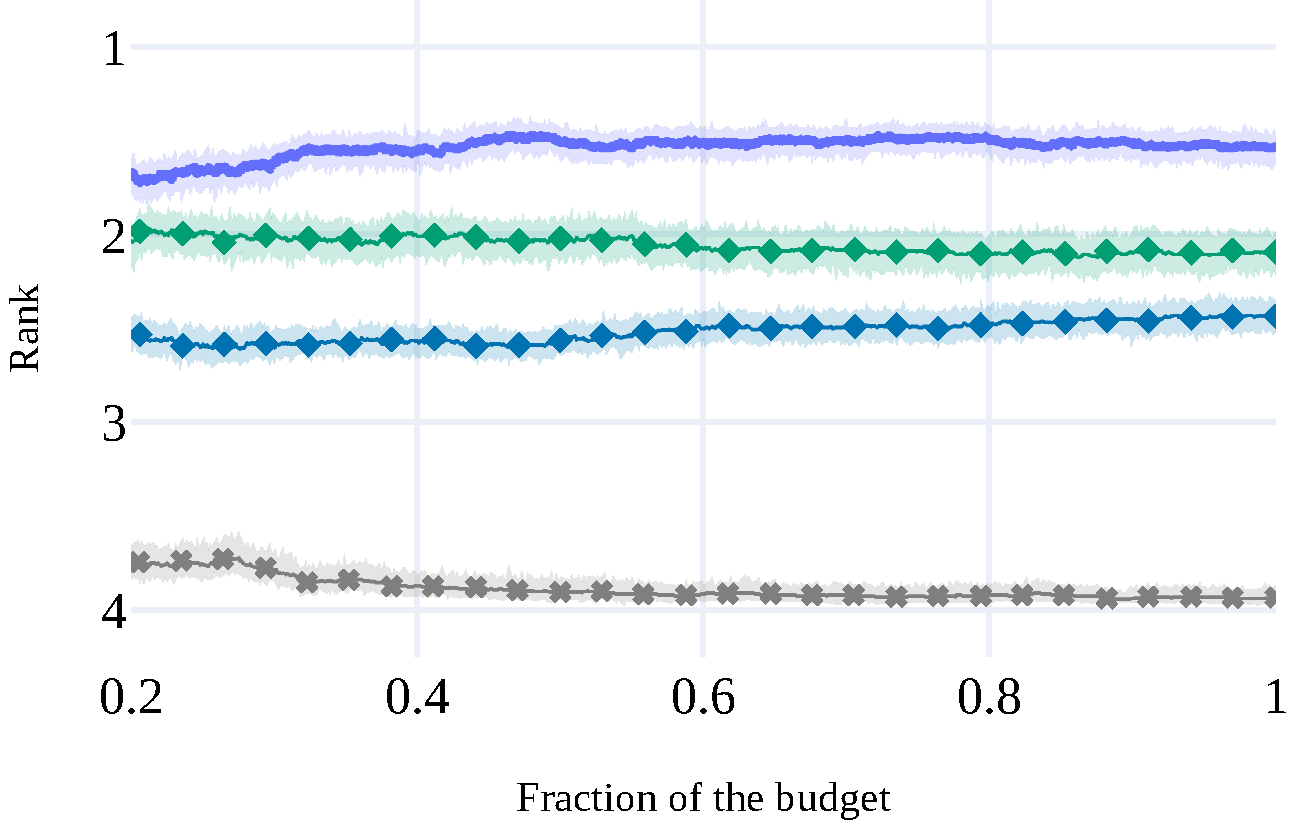
\includegraphics[scale=0.33]{figures/05/figs/figs/ranks/main_ranks_simple2_medium.pdf}
        \caption{Medium-cost (more than 10 minutes, up to \mbox{1 hour})}
    \end{subfigure}
    \begin{subfigure}[t]{0.49\textwidth}
        \centering
        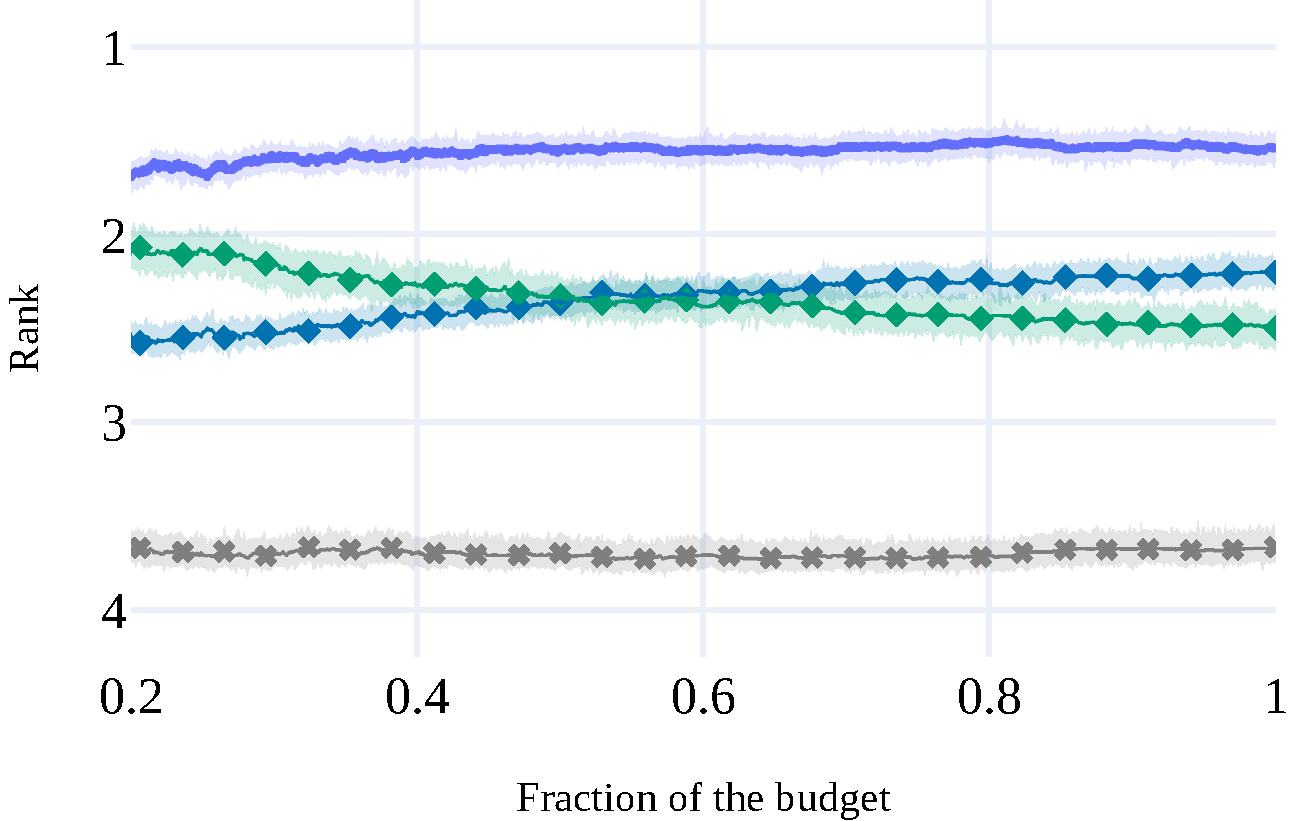
\includegraphics[scale=0.33]{figures/05/figs/figs/ranks/main_ranks_simple2_expensive.pdf}
        \caption{Expensive (more than 1 hour)}
    \end{subfigure}
    \begin{subfigure}[t]{\textwidth}
        \centering
        
\includegraphics[scale=0.33]{figures/05/figs/figs/ranks/main_ranks_simple2_all_legend.pdf}
    \end{subfigure}
    \caption{
    % \hs{
    Mean rank of \texttt{DyMBO} with ($\alpha=1.0$), HEBO with RF and GP surrogates, and random search on YAHPO Gym and JAHS-Bench-201 as a function of the fraction of the wall-clock time budget of each task. Results are shown for (a) all target functions, (b) cheap functions with budgets of up to 10 minutes, (c) medium-cost functions with budgets between 10 minutes and 1 hour, and (d) expensive functions with budgets exceeding 1 hour. Lower ranks indicate better performance. \texttt{DyMBO} achieves the best mean rank in all budget groups, while the relative performance of the RF and GP baselines varies across groups.
    % }
    }
    \label{fig:ch05:gen_res_simple}
\end{figure*}

\begin{figure*}[h]
    \centering
    \begin{subfigure}[t]{0.49\textwidth}
        \centering
        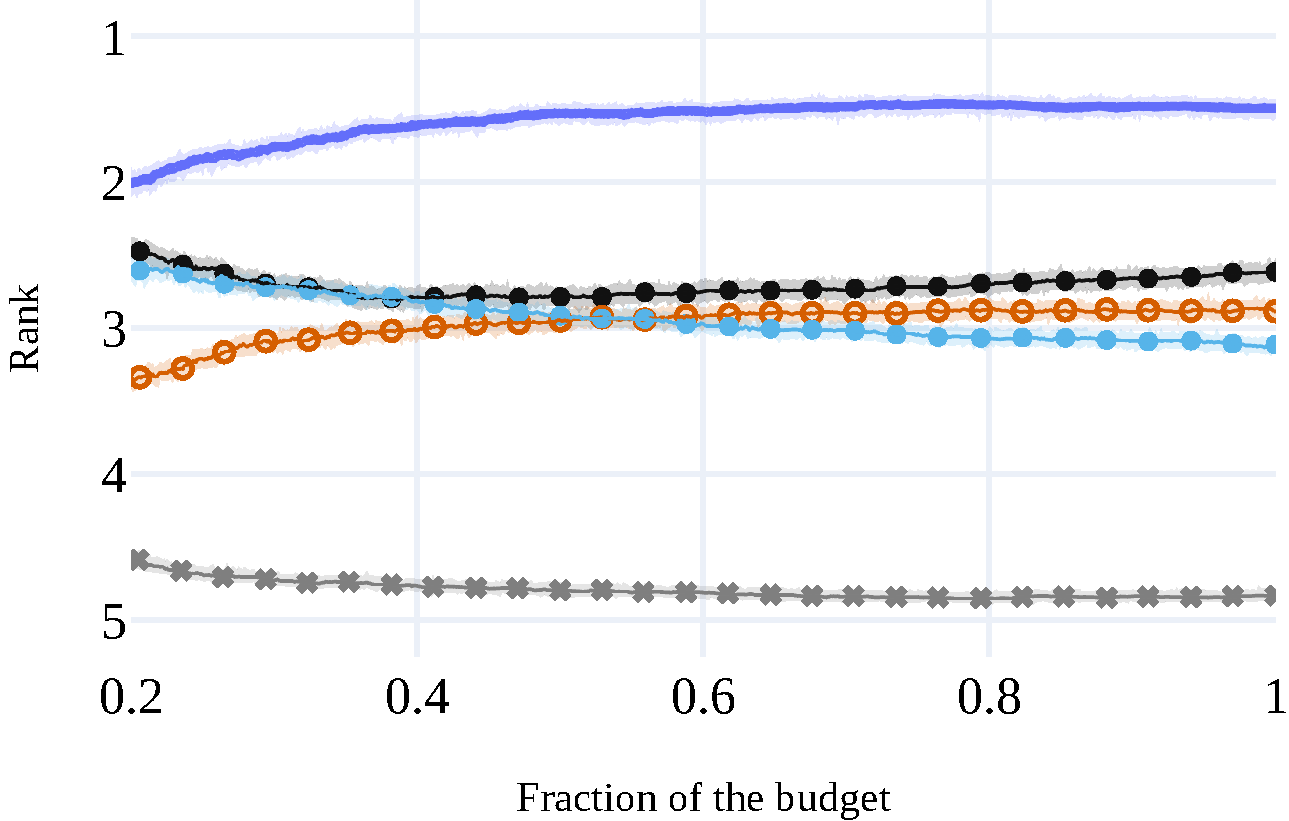
\includegraphics[scale=0.33]{figures/05/figs/figs/ranks/main_ranks_other_baselines2_all.pdf}
        \caption{All target functions}
    \end{subfigure}
    \begin{subfigure}[t]{0.49\textwidth}
        \centering
        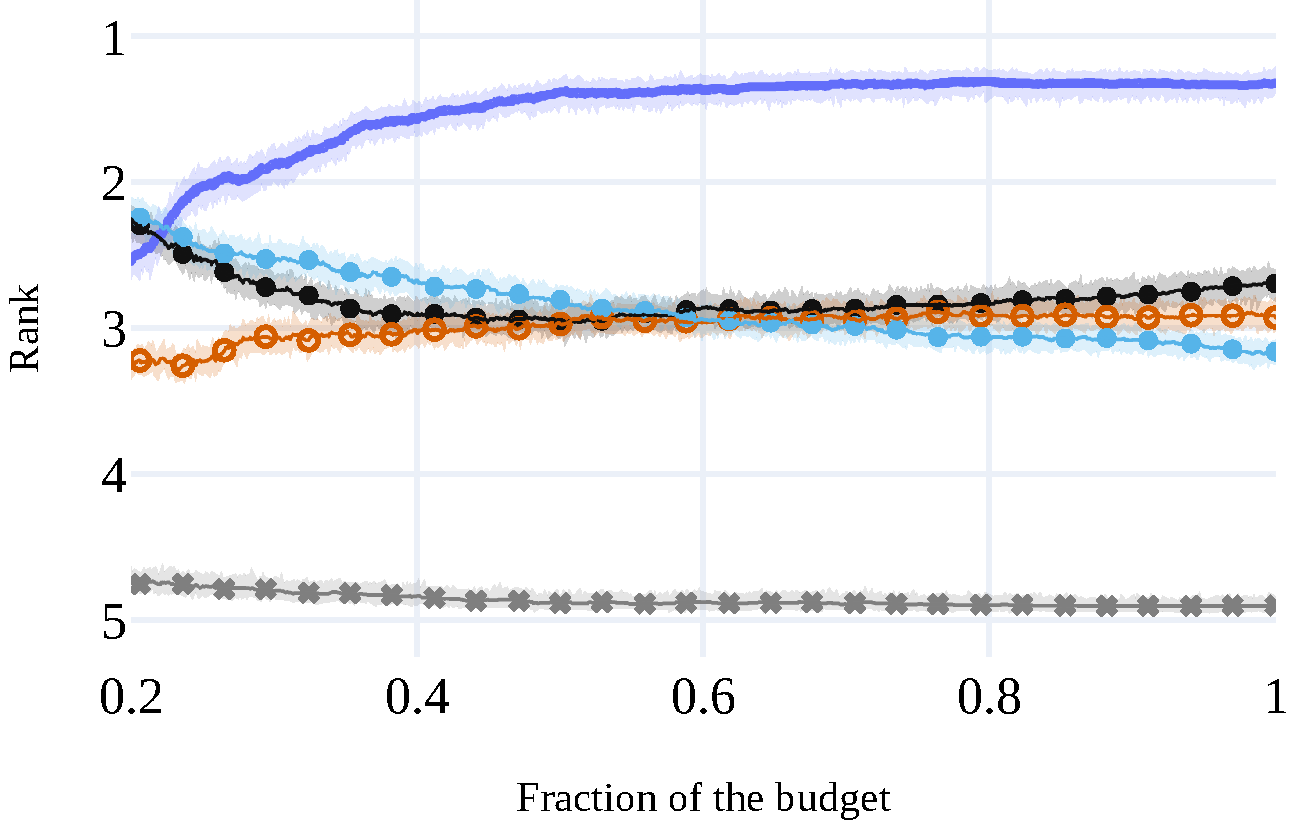
\includegraphics[scale=0.33]{figures/05/figs/figs/ranks/main_ranks_other_baselines2_cheap.pdf}
        \caption{Cheap (up to 10 minutes)}
    \end{subfigure}
    \begin{subfigure}[t]{0.49\textwidth}
        \centering
        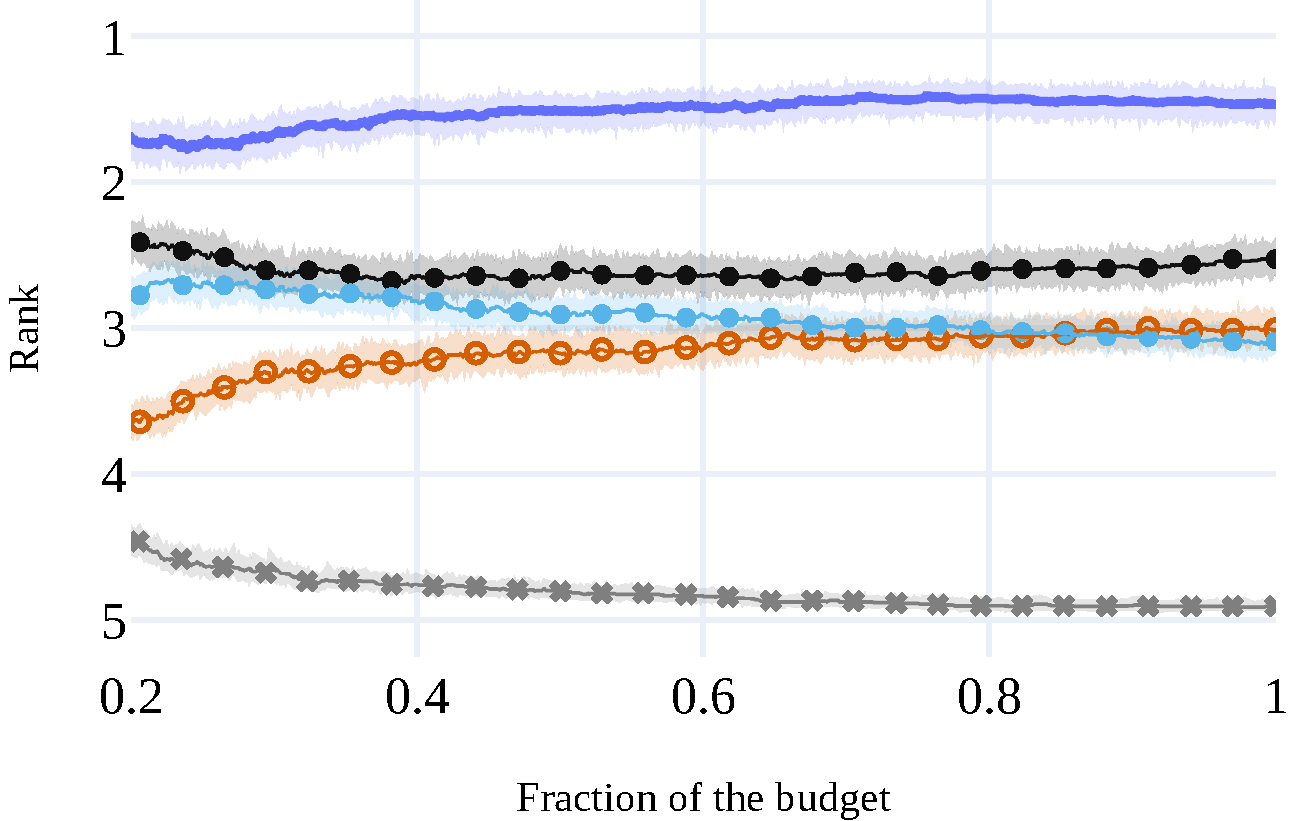
\includegraphics[scale=0.33]{figures/05/figs/figs/ranks/main_ranks_other_baselines2_medium.pdf}
        \caption{Medium-cost (more than 10 minutes, up to \mbox{1 hour})}
    \end{subfigure}
    \begin{subfigure}[t]{0.49\textwidth}
        \centering
        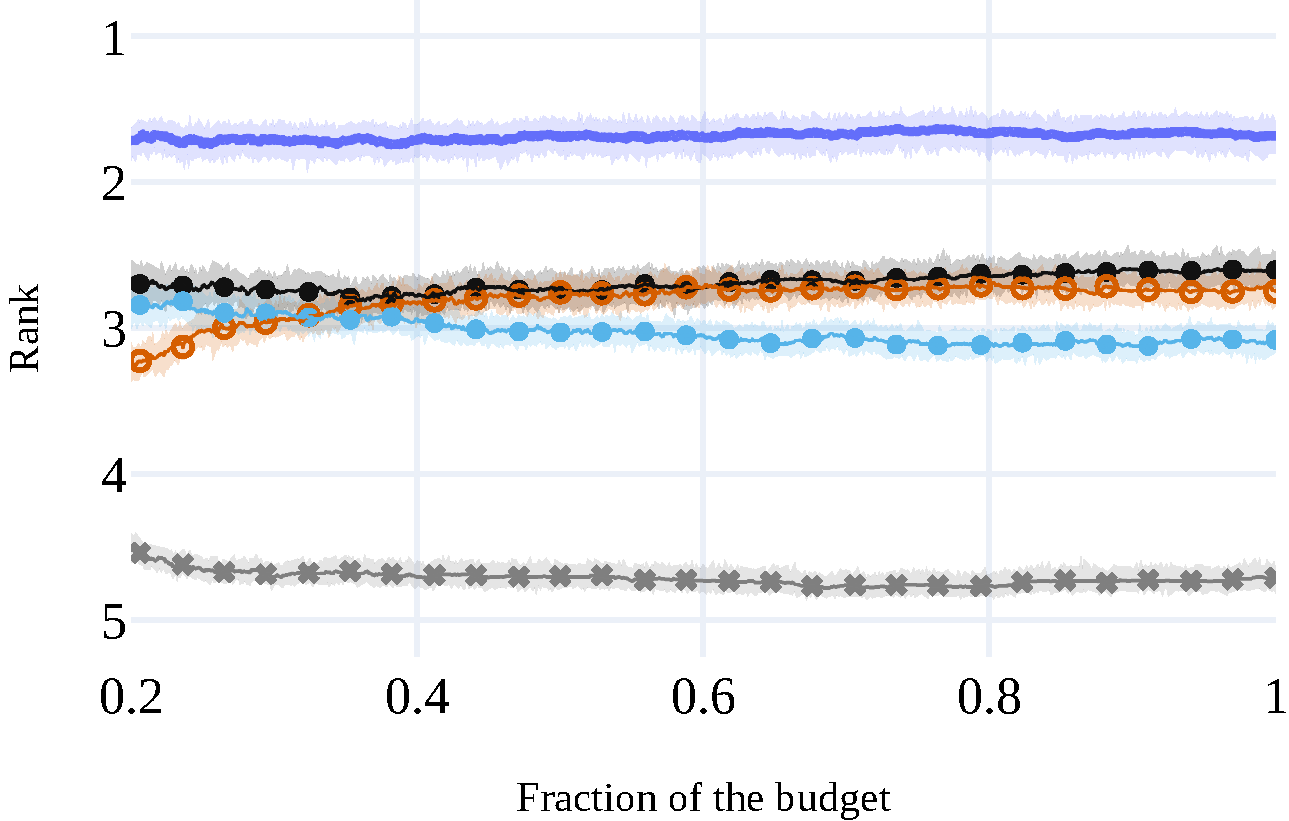
\includegraphics[scale=0.33]{figures/05/figs/figs/ranks/main_ranks_other_baselines2_expensive.pdf}
        \caption{Expensive (more than 1 hour)}
    \end{subfigure}
    \begin{subfigure}[t]{\textwidth}
        \centering
        
\includegraphics[scale=0.33]{figures/05/figs/figs/ranks/main_ranks_other_baselines2_all_legend.pdf}
    \end{subfigure}
    \caption{
    Mean rank of \texttt{DyMBO} with ($\alpha=1.0$), SMAC, Optuna AutoSampler, Optuna TPE, and random search on YAHPO Gym and JAHS-Bench-201 as a function of the fraction of the wall-clock time budget of each task. Results are shown for (a) all target functions, (b) cheap functions with budgets of up to 10 minutes, (c) medium-cost functions with budgets between 10 minutes and 1 hour, and (d) expensive functions with budgets exceeding 1 hour. Lower ranks indicate better performance. \texttt{DyMBO} achieves the best mean rank throughout the optimisation across all budget groups.
    }
    \label{fig:ch05:gen_res_baselines}
\end{figure*}

% \hs{
We continue our evaluation by comparing the best \texttt{DyMBO} variant with HEBO with single surrogates, which is shown in~\cref{fig:ch05:gen_res_simple}.
The results demonstrate that \texttt{DyMBO} achieves a better mean rank compared the HEBO with RF and GP across all budget categories. While for cheap and medium-cost functions GP works well, for the expensive functions, RF works well when more than $50\%$ of the budget has been spent, showing the performance complementarity between the different surrogates. As expected, random search consistently performs worst. Comparing \texttt{DyMBO} to additional baselines, namely TPE as implemented in Optuna, AutoSampler of Optuna and SMAC, we observe in~\cref{fig:ch05:gen_res_baselines} that \texttt{DyMBO} outperforms all of these baselines on average, as SMAC emerges as the second best method, followed by Optuna AutoSampler and Optuna TPE.
% }
% \aj{unresolved ref for fig}

% \er{Can you remind me the reason why we choose the total budget based on time and not evaluations?}\hs{it's HPO, that's a common practice: if we use more time for the optimiser we have less time for the target function}
% We also present an analysis of the statistical significance of our results. 


\begin{figure}[h]
    \centering
    \begin{subfigure}[t]{0.49\textwidth}
        \centering
        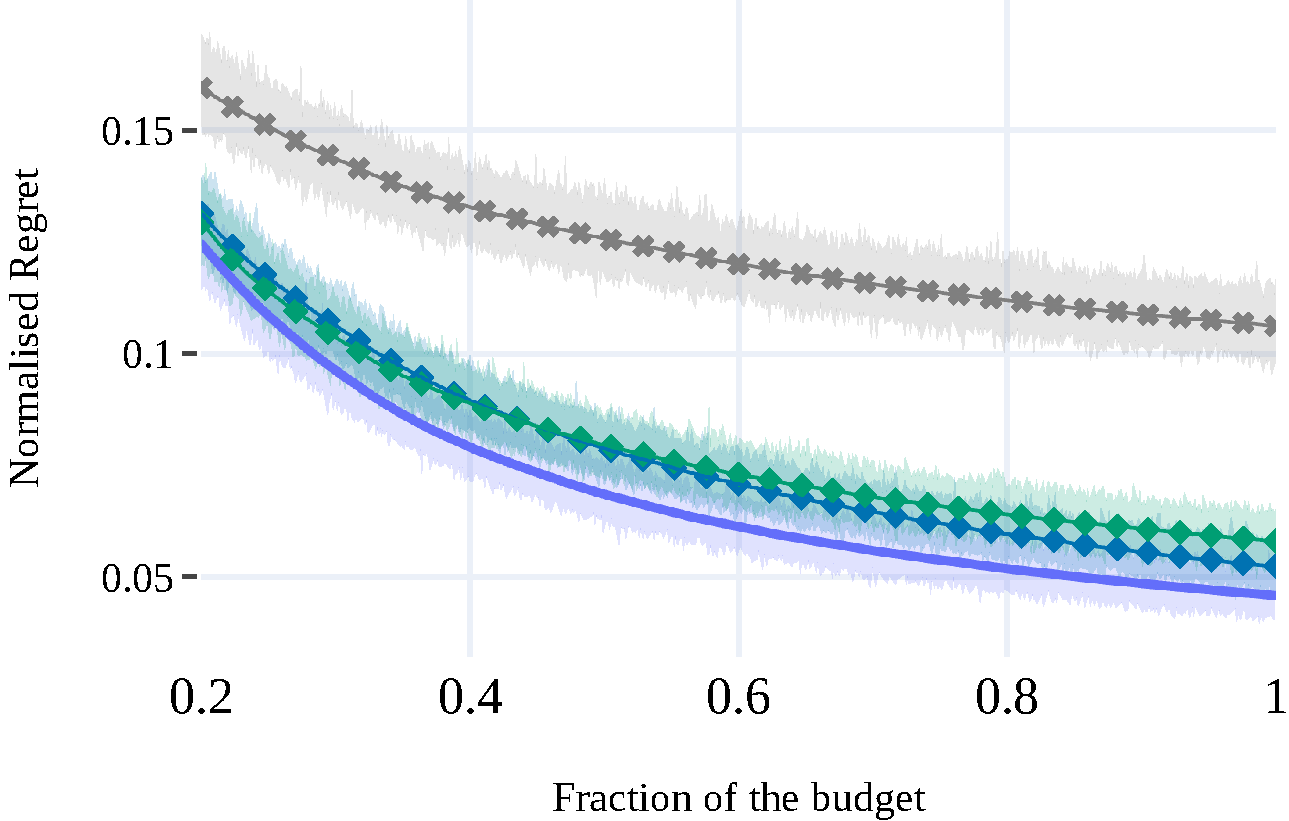
\includegraphics[scale=0.33]{figures/05/figs/figs/ranks/main_ranks_simple2_all_val.pdf}
        \caption{}
    \end{subfigure}
    \begin{subfigure}[t]{0.49\textwidth}
        \centering
        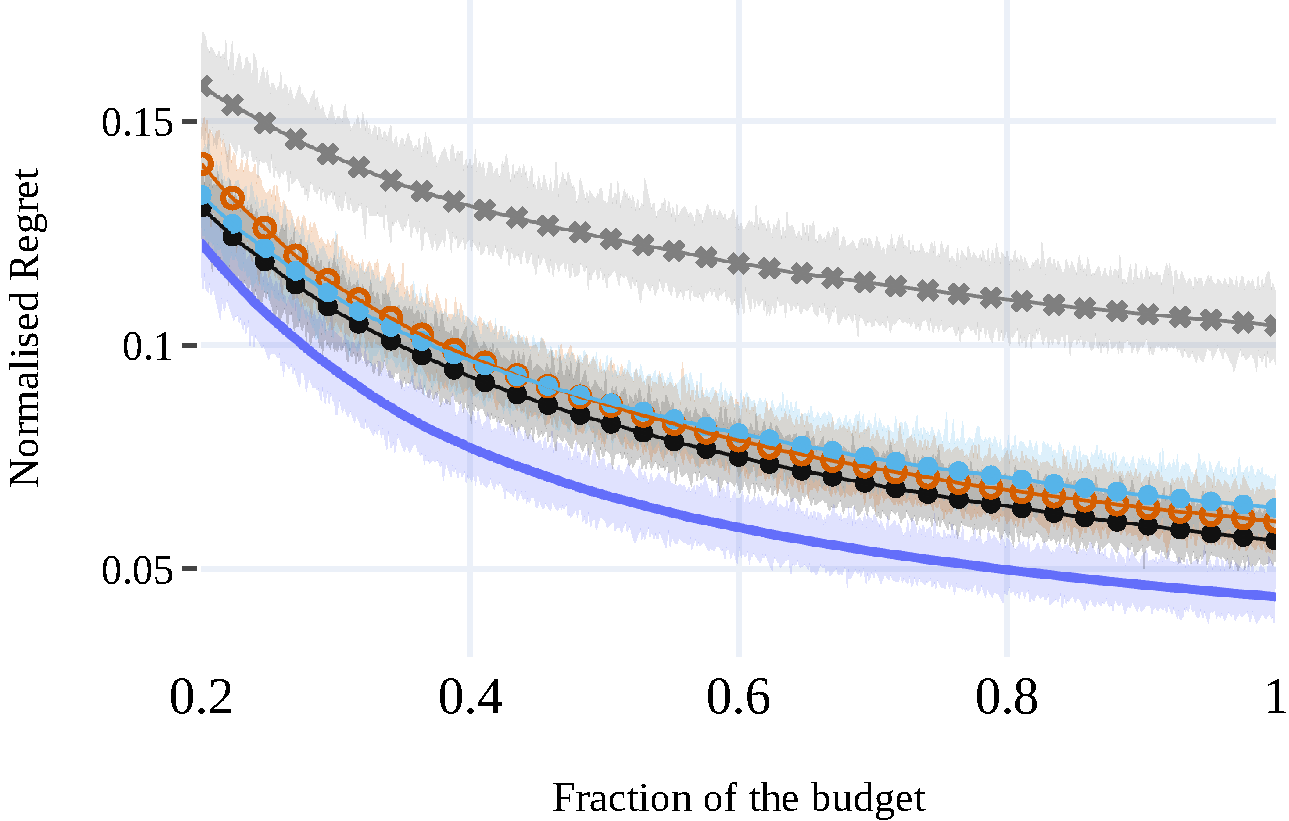
\includegraphics[scale=0.33]{figures/05/figs/figs/ranks/main_ranks_other_baselines2_all_val.pdf}
        \caption{}
    \end{subfigure}
    \begin{subfigure}[t]{0.49\textwidth}
        \centering
        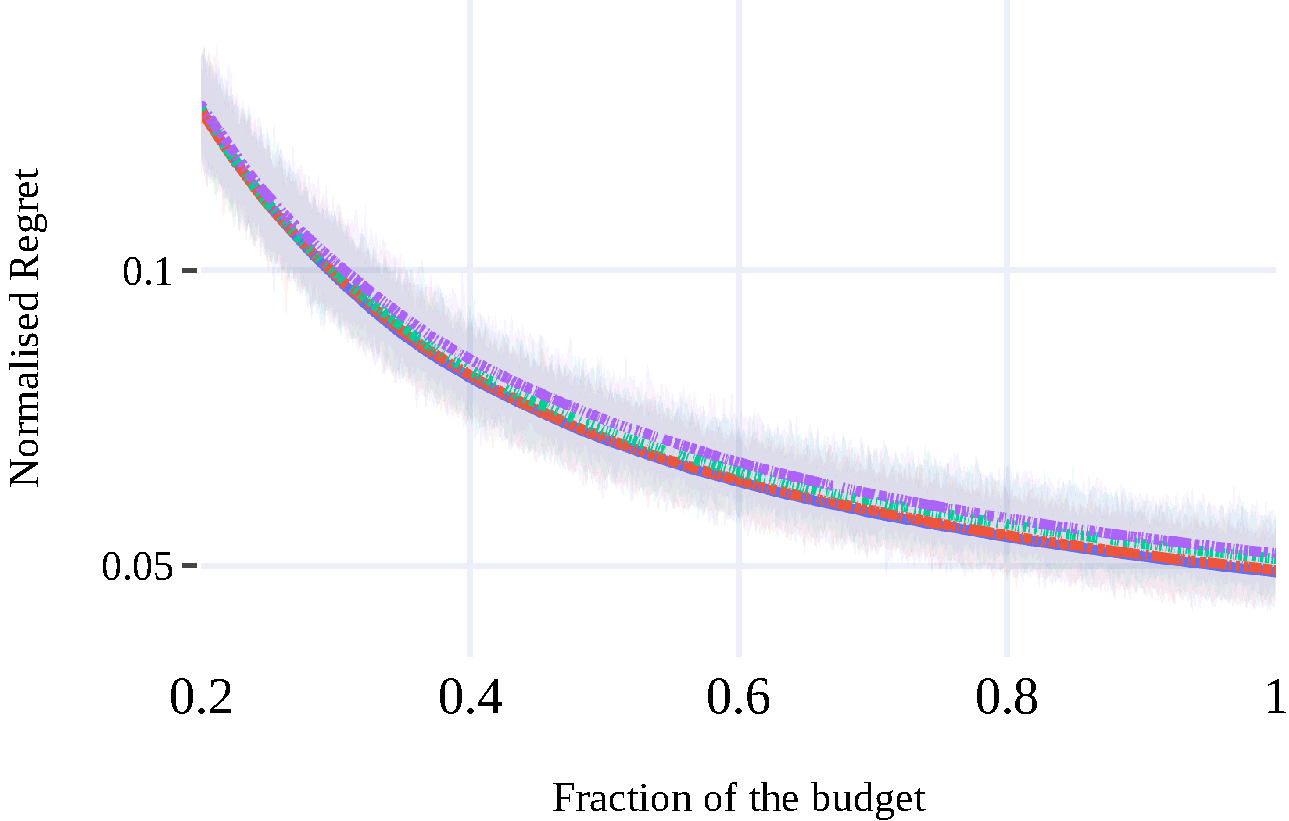
\includegraphics[scale=0.33]{figures/05/figs/figs/ranks/alpha_ablation_all_val.pdf}
        \caption{}
    \end{subfigure}
    \begin{subfigure}[t]{0.49\textwidth}
        \centering
        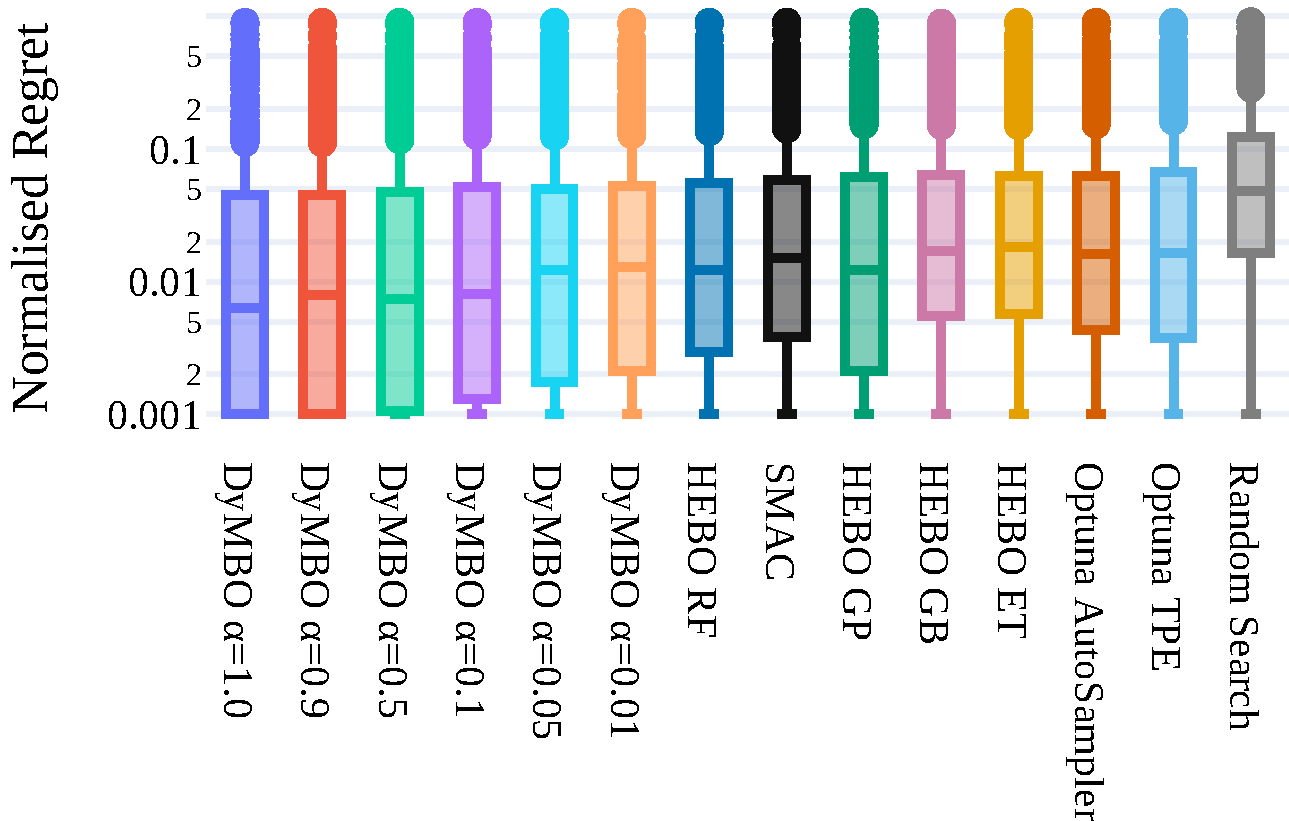
\includegraphics[scale=0.33]{figures/05/figs/figs/ranks/box_plot.pdf}
        \caption{}
    \end{subfigure}
    \begin{subfigure}[t]{\textwidth}
        \centering
        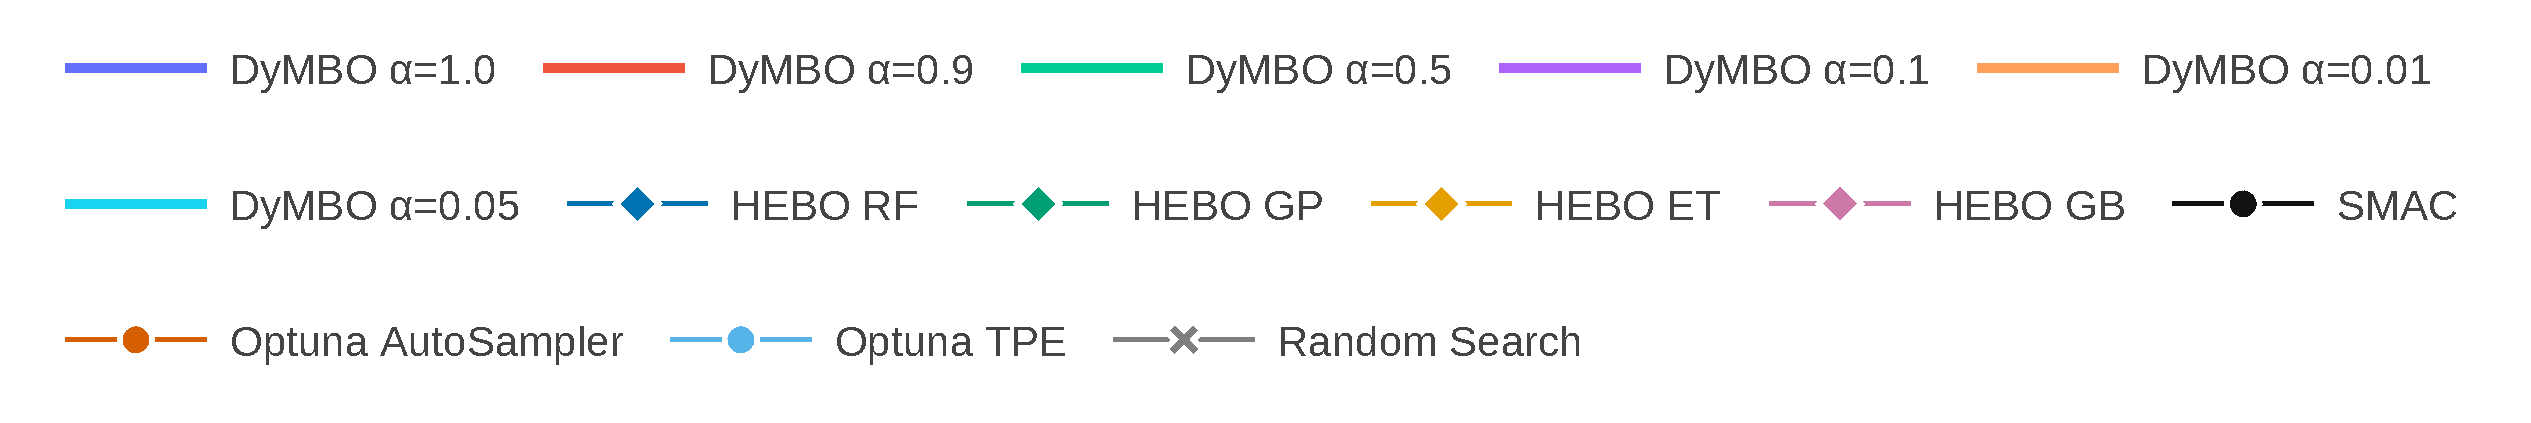
\includegraphics[scale=0.33]{figures/05/figs/figs/ranks/main_ranks_all_val_legend.pdf}
        % \caption{}
    \end{subfigure}
    % 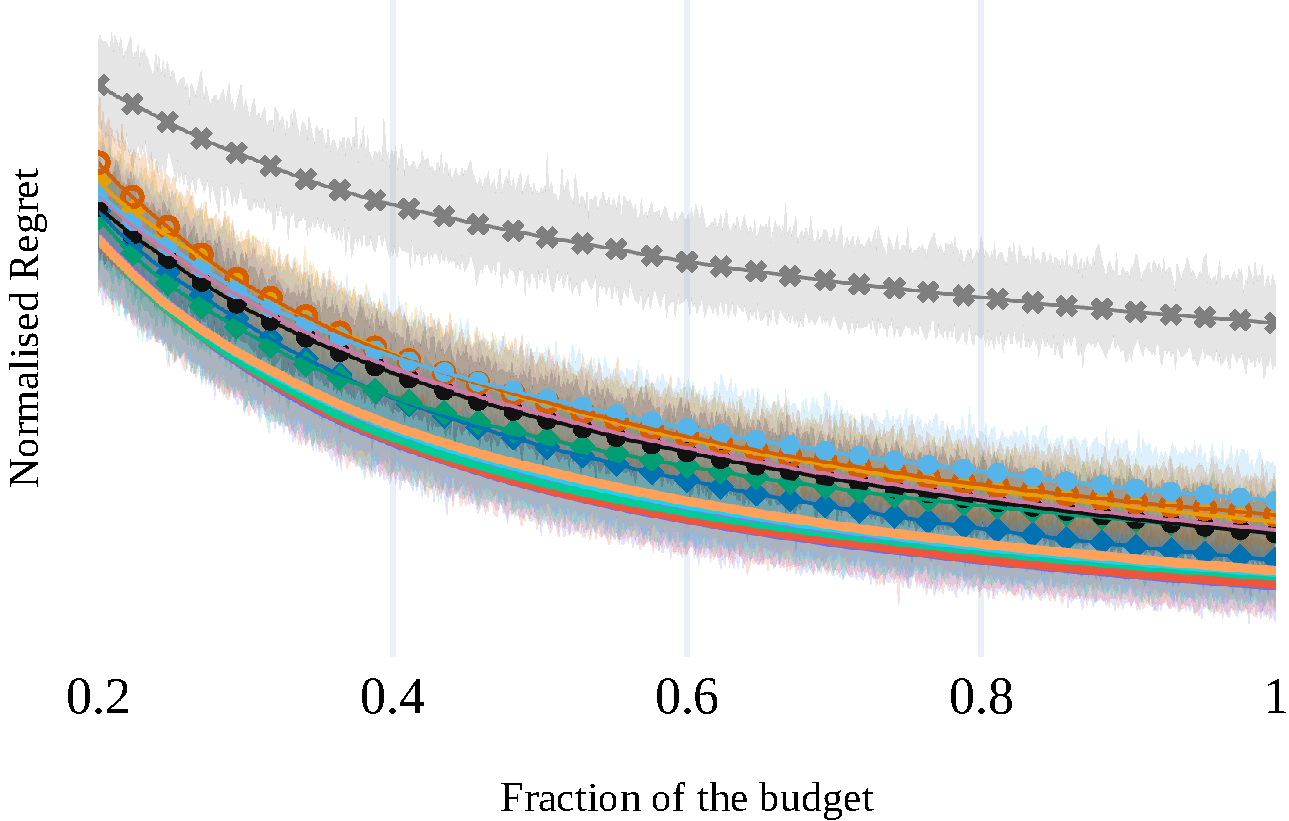
\includegraphics[scale=0.33]{figures/06/figs/figs/ranks/main_ranks_all_val.pdf}
    \caption{%\changed{
    Normalised regret on YAHPO Gym and JAHS-Bench-201 as a function of the fraction of the wall-clock time budget of each task. Panels compare (a) \texttt{DyMBO} with $\alpha=1.0$ against single-surrogate HEBO variants and random search, (b) \texttt{DyMBO} with $\alpha=1.0$ against other HPO frameworks and random search, and (c) \texttt{DyMBO} variants with different values of $\alpha$. Panel (d) shows the distribution of final normalised regret for all methods on a logarithmic scale. Lower normalised regret indicates better performance. \texttt{DyMBO} with $\alpha=1.0$ attains the lowest mean regret and a favourable distribution of final regret relative to the baselines.
    }
    % }
    \label{fig:ch05:mean_reg}
\end{figure}

% \changed{
We present the mean normalised regret of all methods in~\cref{fig:ch05:mean_reg}. Normalised regret is calculated per function, using min-max normalisation with the minimum and maximum value found by all optimisers. 
We performed such normalisation as the values of different functions are in different ranges and scales. We observe lower mean regret for \texttt{DyMBO} compared to the other methods, confirming the results reported by the mean ranks.
% }

% \hh{Minor changes in wording -- check carefully:}
% \changed{
When considering all target functions, we see that \texttt{DyMBO} achieves a better mean rank than the baselines, both those using HEBO and those using other HPO frameworks. When partitioning our set of target functions according to the evaluation budget, we observe different ranks for the single-surrogate HEBO variants. For example, for cheap functions, RF performs better on average than GP on full budget, while GP performs better than RF for the medium budget functions. Despite that, \texttt{DyMBO} is ranked above both HEBO with RFs and HEBO with GPs for all budget categories.

% \changed{The following was in the appendix:}
We tested the statistical significance of our results 
% presented in \autoref{sec:res_general},
% \changed{
and we observe that \texttt{DyMBO} (across both the ensembling and selection variants) 
% }
significantly outperforms single-surrogate-based BO and other considered HPO methods. 
To do this, we used the best-found target function values per optimiser. 
We then calculated the mean value for each pair of function and optimiser over the 51 random seeds. 
The optimiser that has the best value per function is then considered as the best for the particular function. 
We calculated whether the values obtained for each of the other optimisers are statistically equal to the values of the best optimiser using a permutation test with 10\,000 samples and a significance level of $0.05$. 
We report these results in~\cref{tab:ch05:stat_signif}. 
We see that \texttt{DyMBO} achieves equal performance to the best method more times than any other baseline, across all budget groups. 
\texttt{DyMBO} with $\alpha = 1.0$ is statistically tied with the best method in 724 cases, followed by a monotonically decreasing number of ties as $\alpha$ decreases, but remaining statistically significantly better than non-\texttt{DyMBO} methods.
% second-best
The best non-\texttt{DyMBO} method is HEBO using GP with 363 cases. We performed the Wilcoxon sign test on the results of the permutations test, such that for every benchmark we assign 1 when the method is statistically tied with the best method, otherwise we assign 0. We found that 
% \changed{
all variants of \texttt{DyMBO} with different $\alpha$ values are significantly better than all other baselines.
We therefore conclude that \texttt{DyMBO} significantly outperforms any other baseline.
% }

\begin{table}[h]
    \centering
        \caption{
        Win/tie counts of different BO-based approaches, including \texttt{DyMBO}, single-surrogate HEBO baselines, and other HPO methods, per function category (\emph{i.e.}, all, cheap, medium-cost, and expensive functions).
        We report the number of benchmark instances (out of the total across all seeds and functions) for which the method is statistically indistinguishable from the best-performing method under a permutation test with a significance level of $0.05$. All \texttt{DyMBO} variants are significantly better than any other baseline.
        % \aj{Table 1 conspicuously lacks a static ensemble baseline or an explicitly greedy ensemble baseline.}
        % \todo{add these baselines if available, I hope we can run them if not}\hs{we have the results (appendix E). In this figure we only compare to previously published baselines. Will add significance to it as well}
        % \todo{Critical difference usually shows the difference in mean ranks and if they are pairwise significant. Could the authors please explain more about how to read Table 1?}
        }

    \begin{tabular}{llrrrr}
\toprule
Model & All & Cheap & Medium & Expensive \\
\midrule
 DyMBO $\alpha=0.1$ & 518 & 156 & 158 & 204 \\
 DyMBO $\alpha=0.5$ & 678 & 238 & 190 & 250 \\
 DyMBO $\alpha=0.9$ & 714 & 261 & 193 & \textbf{260} \\
 DyMBO $\alpha=1.0$ & \textbf{724} & \textbf{272} & \textbf{200} & 252 \\
 ET & 142 & 32 & 57 & 53 \\
 GB & 113 & 19 & 28 & 66 \\
 GP & 363 & 103 & 133 & 127 \\
 RF & 277 & 63 & 84 & 130 \\
 Optuna AutoSampler & 181 & 45 & 38 & 98 \\
 Optune TPE & 139 & 26 & 32 & 81 \\
 Random Search & 35 & 6 & 0 & 29 \\
 SMAC & 222 & 47 & 65 & 110 \\
\bottomrule
\end{tabular}
    \label{tab:ch05:stat_signif}
\end{table}

All figures (convergence plots, weight evolution and performance comparison), including results for JAHS-Bench-201, are available in the supplemental Git repository (see~\cref{sec:code-availability})
due to reasons of space.
% as there are 859 such figures. 
We provide convergence plots in~\cref{fig:ch05:full_res,fig:ch05:full_res2} for a subset of YAHPO Gym, namely the YAHPO-SO benchmark suite that contains 20 HPO problems from different scenarios. 
Additionally, we provide results for raw benchmarks (such as HPOBench) and synthetic benchmarks in~\cref{sec:ch05:add-bench}.


% \section{Weights evolution}

\begin{figure*}
    \centering
   
\begin{subfigure}[t]{0.32\textwidth}
        \centering
        \includegraphics[scale=0.33]{figures/05/figs/figs/co/co_8_init_srbv2\_rparti40499_time.pdf}
        \caption{rbv2\_rpart 40499}
    \end{subfigure}
\begin{subfigure}[t]{0.32\textwidth}
        \centering
        \includegraphics[scale=0.33]{figures/05/figs/figs/co/co_8_init_srbv2\_superi1053_time.pdf}
        \caption{rbv2\_super 1053}
    \end{subfigure}
\begin{subfigure}[t]{0.32\textwidth}
        \centering
        \includegraphics[scale=0.33]{figures/05/figs/figs/co/co_8_init_srbv2\_superi1457_time.pdf}
        \caption{rbv2\_super 1457}
    \end{subfigure}
\begin{subfigure}[t]{0.32\textwidth}
        \centering
        \includegraphics[scale=0.33]{figures/05/figs/figs/co/co_8_init_srbv2\_superi1063_time.pdf}
        \caption{rbv2\_super 1063}
    \end{subfigure}
\begin{subfigure}[t]{0.32\textwidth}
        \centering
        \includegraphics[scale=0.33]{figures/05/figs/figs/co/co_8_init_srbv2\_superi1479_time.pdf}
        \caption{rbv2\_super 1479}
    \end{subfigure}
\begin{subfigure}[t]{0.32\textwidth}
        \centering
        \includegraphics[scale=0.33]{figures/05/figs/figs/co/co_8_init_srbv2\_superi15_time.pdf}
        \caption{rbv2\_super 15}
    \end{subfigure}
\begin{subfigure}[t]{0.32\textwidth}
        \centering
        \includegraphics[scale=0.33]{figures/05/figs/figs/co/co_8_init_srbv2\_superi1468_time.pdf}
        \caption{rbv2\_super 1468}
    \end{subfigure}
\begin{subfigure}[t]{0.32\textwidth}
        \centering
        \includegraphics[scale=0.33]{figures/05/figs/figs/co/co_8_init_srbv2\_xgboosti12_time.pdf}
        \caption{rbv2\_xgboost 12}
    \end{subfigure}
\begin{subfigure}[t]{0.32\textwidth}
        \centering
        \includegraphics[scale=0.33]{figures/05/figs/figs/co/co_8_init_srbv2\_xgboosti1501_time.pdf}
        \caption{rbv2\_xgboost 1501}
    \end{subfigure}
\begin{subfigure}[t]{0.32\textwidth}
        \centering
        \includegraphics[scale=0.33]{figures/05/figs/figs/co/co_8_init_srbv2\_xgboosti16_time.pdf}
        \caption{rbv2\_xgboost 16}
    \end{subfigure}
\begin{subfigure}[t]{0.32\textwidth}
        \centering
        \includegraphics[scale=0.33]{figures/05/figs/figs/co/co_8_init_srbv2\_xgboosti40499_time.pdf}
        \caption{rbv2\_xgboost 40499}
    \end{subfigure}
    \begin{subfigure}[t]{1.0\textwidth}
        \centering
        \includegraphics[scale=0.33]{figures/05/figs/figs/co/co_8_init_srbv2\_xgboosti40499_time_legend.pdf.pdf}
    \end{subfigure}
    \caption{Convergence plots of \texttt{DyMBO}, HEBO with GP, HEBO with RF, and random search for the YAHPO-SO subset, as a function of the fraction of the wall-clock time budget for each task. 
    }
    % \todo{}\er{What's happening in subfigure (t) for HEBO?}}
    \label{fig:ch05:full_res}
\end{figure*}


\begin{figure*}
    \centering
    \begin{subfigure}[t]{0.32\textwidth}
        \centering
        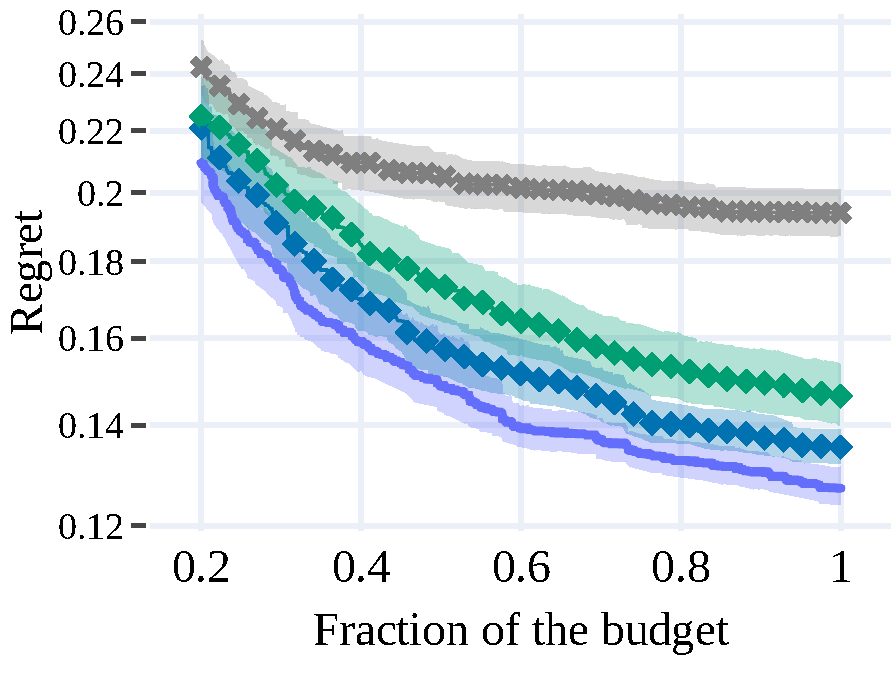
\includegraphics[scale=0.33]{figures/05/figs/figs/co/co_8_init_slcbenchi167168_time.pdf}
        \caption{lcbench 167168}
    \end{subfigure}
\begin{subfigure}[t]{0.32\textwidth}
        \centering
        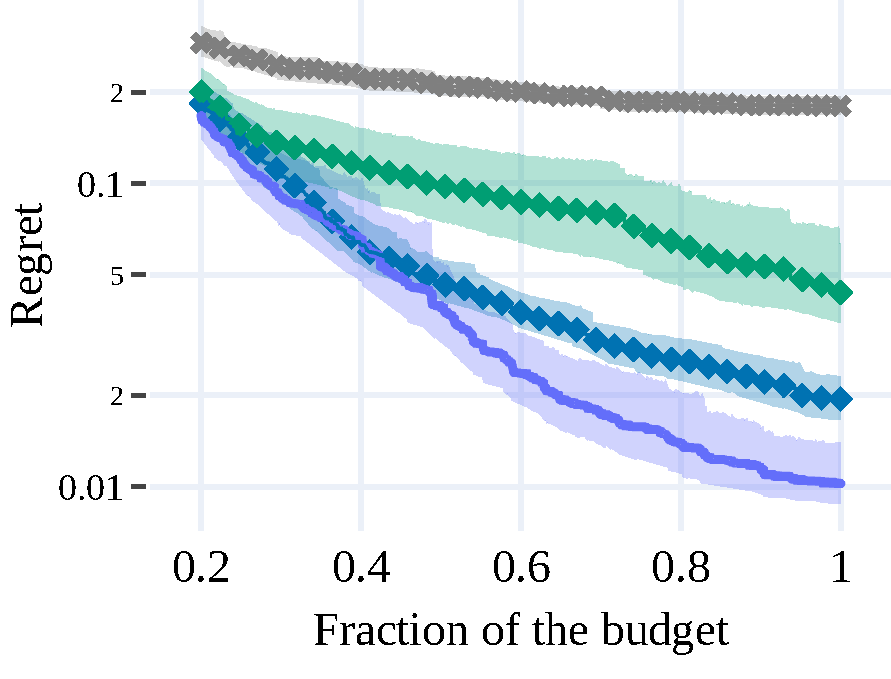
\includegraphics[scale=0.33]{figures/05/figs/figs/co/co_8_init_slcbenchi189873_time.pdf}
        \caption{lcbench 189873}
    \end{subfigure}
\begin{subfigure}[t]{0.32\textwidth}
        \centering
        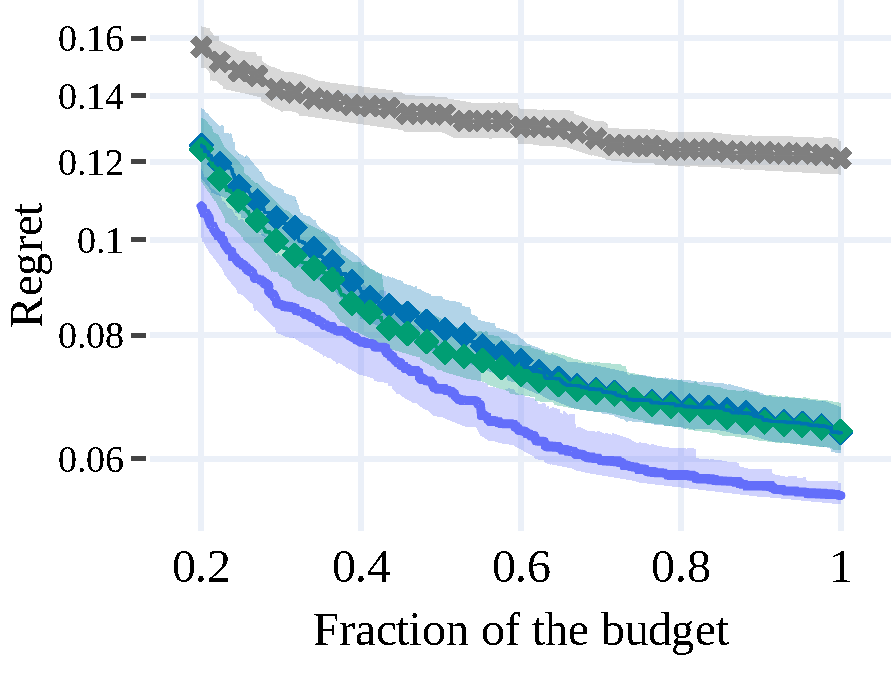
\includegraphics[scale=0.33]{figures/05/figs/figs/co/co_8_init_slcbenchi189906_time.pdf}
        \caption{lcbench 189906}
    \end{subfigure}
\begin{subfigure}[t]{0.32\textwidth}
        \centering
        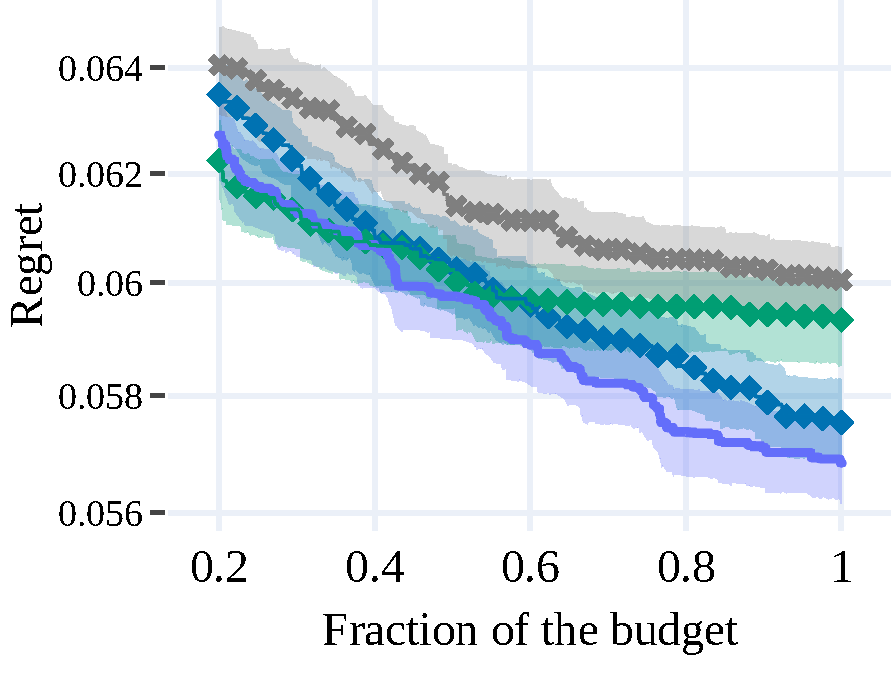
\includegraphics[scale=0.33]{figures/05/figs/figs/co/co_8_init_snb301iCIFAR10_time.pdf}
        \caption{nb301 CIFAR10}
    \end{subfigure}
\begin{subfigure}[t]{0.32\textwidth}
        \centering
        \includegraphics[scale=0.33]{figures/05/figs/figs/co/co_8_init_srbv2\_glmneti375_time.pdf}
        \caption{rbv2\_glmnet 375}
    \end{subfigure}
\begin{subfigure}[t]{0.32\textwidth}
        \centering
        \includegraphics[scale=0.33]{figures/05/figs/figs/co/co_8_init_srbv2\_glmneti458_time.pdf}
        \caption{rbv2\_glmnet 458}
    \end{subfigure}
\begin{subfigure}[t]{0.32\textwidth}
        \centering
        \includegraphics[scale=0.33]{figures/05/figs/figs/co/co_8_init_srbv2\_rangeri16_time.pdf}
        \caption{rbv2\_ranger 16}
    \end{subfigure}
\begin{subfigure}[t]{0.32\textwidth}
        \centering
        \includegraphics[scale=0.33]{figures/05/figs/figs/co/co_8_init_srbv2\_rangeri42_time.pdf}
        \caption{rbv2\_ranger 42}
    \end{subfigure}
\begin{subfigure}[t]{0.32\textwidth}
        \centering
        \includegraphics[scale=0.33]{figures/05/figs/figs/co/co_8_init_srbv2\_rparti14_time.pdf}
        \caption{rbv2\_rpart 14}
    \end{subfigure}


    \begin{subfigure}[t]{1.0\textwidth}
        \centering
        \includegraphics[scale=0.33]{figures/05/figs/figs/co/co_8_init_srbv2\_xgboosti40499_time_legend.pdf}
    \end{subfigure}
    \caption{Convergence plots of \texttt{DyMBO}, HEBO with GP, HEBO with RF, and random search for the YAHPO-SO subset, as a function of the fraction of the wall-clock time budget for each task (continued from~\cref{fig:ch05:full_res}).
    % \er{In the x-axis label, the g of budget is often cut. This actually happens in many other figures too (like Fig. 6)}.
    }
    % \todo{}\er{What's happening in subfigure (t) for HEBO?}}
    \label{fig:ch05:full_res2}
\end{figure*}





\subsection{Running time}
\label{sec:ch05:running_time}

\begin{figure*}[h!]
    \centering
    \begin{subfigure}[t]{0.49\textwidth}
        \centering
        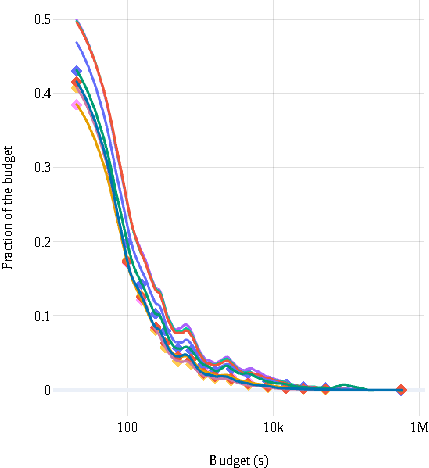
\includegraphics[width=\textwidth]{figures/05/figs/figs/time_percent.pdf}
        \caption{Fraction of budget (in seconds)}
        \label{fig:ch05:rt_frac_of_bud}
    \end{subfigure}
    \begin{subfigure}[t]{0.49\textwidth}
        \centering
        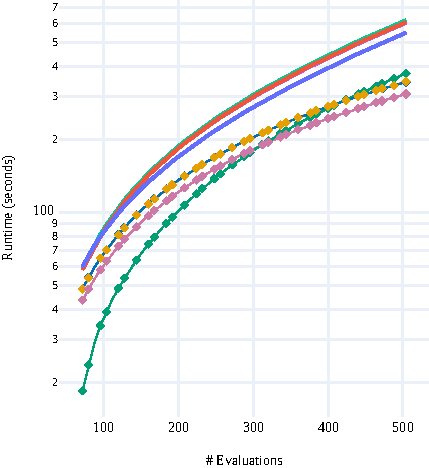
\includegraphics[width=\textwidth]{figures/05/figs/figs/time/nb301_time.pdf}
        \caption{Absolute running time}
        \label{fig:ch05:rt_absolute}
    \end{subfigure}

\includegraphics[width=\textwidth]{figures/05/figs/figs/time/nb301_time_legend.pdf}
    \caption{
    Running time of the optimisation with \texttt{DyMBO} (excluding the time needed to evaluate the target function): (a) as a fraction of optimisation budget, and (b) as absolute running time relative to the number of target function evaluations. Ensembles generally require a higher fraction of the budget compared to single surrogates and take the longest to run in absolute terms, with a notable exception of the ensemble with $\alpha=1.0$, which 
    consumes less budget by an order of magnitude, and which is the fastest to run, due to dynamic pruning. 
    }
    \label{fig:ch05:running-times}
\end{figure*}

We assessed the wall-clock time used by the optimiser itself, \emph{i.e.,} excluding the time required to evaluate the target function, as a percentage of the optimisation budget and as absolute running time relative to the number of target function evaluations. 
\cref{fig:ch05:rt_frac_of_bud} shows the proportion of the optimisation budget (in seconds)
used by the optimiser to suggest the next configurations to sample across all YAHPO Gym functions. 
As expected, for very low budgets (up to approximately 20 seconds), the optimiser consumes a high fraction of the budget (more than 35\%). 
As the budget increases, this fraction decreases, until it becomes negligible (less than 1\% for budgets of more than 10\,000 seconds).
We observe that using ensembles requires a higher fraction of the optimisation budget than using a single surrogate. 
However, the difference becomes indistinguishable when the budget exceeds 1\,000 seconds. 
% When using dynamic ensembling with $\alpha=1.0$, the difference becomes difficult to discern even with a budget of 1\,000 seconds, once more demonstrating the effectiveness of dynamic pruning of surrogate models.

% \hh{minor changes -- check:}
% \changed{
Additionally, we assessed the absolute cost of using different surrogates on the benchmark NAS-Bench-301 from YAHPO Gym, considering up to 512 evaluations. The results are presented in~\cref{fig:ch05:rt_absolute}. 
We first observe that \texttt{DyMBO} 
% \er{It's the second time I find the plural, why? We show one version of DyMBO on that figure.} 
takes the longest to run, although the gap from the single-surrogate HEBO variants is not large, at around 150 seconds for 512 evaluations; this is a relatively short time given that each evaluation of the target function takes around one hour. For lower numbers of evaluations, the gap is even smaller.
% We also notice that ensembling approaches take roughly twice as long as tree-based surrogates. 
GPs are the fastest to run with a low number of evaluations, however the gap between them and tree-based methods shrinks substantially as more observations are added.
% }



\subsection{Evolution of weights}
\label{sec:ch05:weights}

We show the evolution of the weights of the surrogate models in the ensemble over the course of the optimisation in~\cref{fig:ch05:weights}. 
To this end, we made use of the data from the experiment with fixed 512 evaluations as described in~\cref{sec:ch05:diff_exp_setup}, with GP and RF as surrogate models.
% We show the results in. 
% \changed{
We observe that the weights of the surrogates change rapidly and frequently during the optimisation process, \emph{i.e.}, the weights are not constant, and the surrogates are not used equally. 
This indicates that neither surrogate consistently dominates 
and that the relative predictive performance of GP and RF alternates across iterations.
This switching behaviour justifies the use of a dynamic ensemble over simply choosing a single surrogate model at the start of optimisation.

We also see different weight dynamics, depending on the given target function. 
% \hh{better: optimised? or ... on the given target function?}.
On some target functions, \emph{e.g.,}~\cref{fig:ch05:weights}(c, p, q), GP is assigned a near-constant weight of $1$ for the majority of the optimisation process, suggesting a strong and 
stable preference for GP on these problems.
On the target function in~\cref{fig:ch05:weights}(n), it is RF that consistently dominates the optimisation with a near-constant weight of $1$.
In contrast, on most other target functions, the weights oscillate frequently between the two surrogates, indicating that both GP and RF contribute meaningfully and that neither is uniformly superior.
Furthermore, the onset of switching behaviour varies substantially depending on the target function.
% }
% \todo{Could the authors kindly add their insight(s) that the reader could take away from Figure 18?}
% }
\begin{figure*}
    \centering
    \begin{subfigure}[t]{0.24\textwidth}
        \centering
        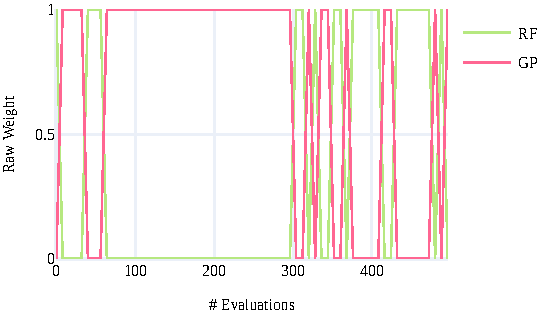
\includegraphics[width=\textwidth]{figures/05/figs/figs/weights/w_2d_init_slcbenchi167168_smens_ranking_loss_rf_gp_init_orf_eval_all.pdf}
        \caption{lcbench 167168}
    \end{subfigure}
\begin{subfigure}[t]{0.24\textwidth}
        \centering
        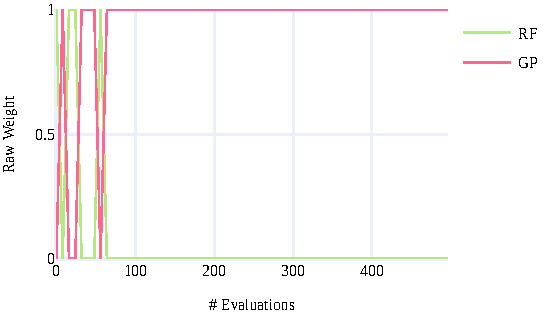
\includegraphics[width=\textwidth]{figures/05/figs/figs/weights/w_2d_init_slcbenchi189873_smens_ranking_loss_rf_gp_init_orf_eval_all.pdf}
        \caption{lcbench 189873}
    \end{subfigure}
\begin{subfigure}[t]{0.24\textwidth}
        \centering
        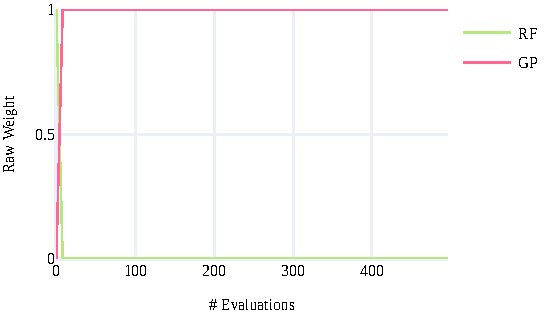
\includegraphics[width=\textwidth]{figures/05/figs/figs/weights/w_2d_init_slcbenchi189906_smens_ranking_loss_rf_gp_init_orf_eval_all.pdf}
        \caption{lcbench 189906}
    \end{subfigure}
\begin{subfigure}[t]{0.24\textwidth}
        \centering
        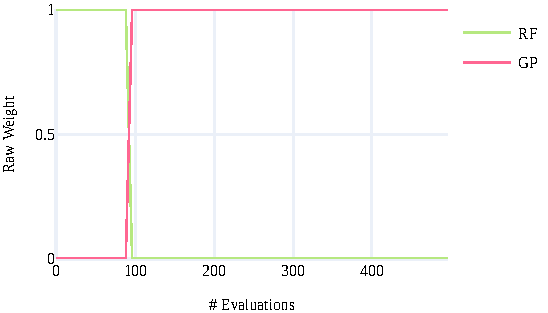
\includegraphics[width=\textwidth]{figures/05/figs/figs/weights/w_2d_init_snb301iCIFAR10_smens_ranking_loss_rf_gp_init_orf_eval_all.pdf}
        \caption{nb301 CIFAR10}
    \end{subfigure}
\begin{subfigure}[t]{0.24\textwidth}
        \centering
        \includegraphics[width=\textwidth]{figures/05/figs/figs/weights/w_2d_init_srbv2\_glmneti375_smens_ranking_loss_rf_gp_init_orf_eval_all.pdf}
        \caption{rbv2\_glmnet 375}
    \end{subfigure}
\begin{subfigure}[t]{0.24\textwidth}
        \centering
        \includegraphics[width=\textwidth]{figures/05/figs/figs/weights/w_2d_init_srbv2\_glmneti458_smens_ranking_loss_rf_gp_init_orf_eval_all.pdf}
        \caption{rbv2\_glmnet 458}
    \end{subfigure}
\begin{subfigure}[t]{0.24\textwidth}
        \centering
        \includegraphics[width=\textwidth]{figures/05/figs/figs/weights/w_2d_init_srbv2\_rangeri16_smens_ranking_loss_rf_gp_init_orf_eval_all.pdf}
        \caption{rbv2\_ranger 16}
    \end{subfigure}
\begin{subfigure}[t]{0.24\textwidth}
        \centering
        \includegraphics[width=\textwidth]{figures/05/figs/figs/weights/w_2d_init_srbv2\_rangeri42_smens_ranking_loss_rf_gp_init_orf_eval_all.pdf}
        \caption{rbv2\_ranger 42}
    \end{subfigure}
\begin{subfigure}[t]{0.24\textwidth}
        \centering
        \includegraphics[width=\textwidth]{figures/05/figs/figs/weights/w_2d_init_srbv2\_rparti14_smens_ranking_loss_rf_gp_init_orf_eval_all.pdf}
        \caption{rbv2\_rpart 14}
    \end{subfigure}
\begin{subfigure}[t]{0.24\textwidth}
        \centering
        \includegraphics[width=\textwidth]{figures/05/figs/figs/weights/w_2d_init_srbv2\_rparti40499_smens_ranking_loss_rf_gp_init_orf_eval_all.pdf}
        \caption{rbv2\_rpart 40499}
    \end{subfigure}
\begin{subfigure}[t]{0.24\textwidth}
        \centering
        \includegraphics[width=\textwidth]{figures/05/figs/figs/weights/w_2d_init_srbv2\_superi1053_smens_ranking_loss_rf_gp_init_orf_eval_all.pdf}
        \caption{rbv2\_super 1053}
    \end{subfigure}
\begin{subfigure}[t]{0.24\textwidth}
        \centering
        \includegraphics[width=\textwidth]{figures/05/figs/figs/weights/w_2d_init_srbv2\_superi1457_smens_ranking_loss_rf_gp_init_orf_eval_all.pdf}
        \caption{rbv2\_super 1457}
    \end{subfigure}
\begin{subfigure}[t]{0.24\textwidth}
        \centering
        \includegraphics[width=\textwidth]{figures/05/figs/figs/weights/w_2d_init_srbv2\_superi1063_smens_ranking_loss_rf_gp_init_orf_eval_all.pdf}
        \caption{rbv2\_super 1063}
    \end{subfigure}
\begin{subfigure}[t]{0.24\textwidth}
        \centering
        \includegraphics[width=\textwidth]{figures/05/figs/figs/weights/w_2d_init_srbv2\_superi1479_smens_ranking_loss_rf_gp_init_orf_eval_all.pdf}
        \caption{rbv2\_super 1479}
    \end{subfigure}
\begin{subfigure}[t]{0.24\textwidth}
        \centering
        \includegraphics[width=\textwidth]{figures/05/figs/figs/weights/w_2d_init_srbv2\_superi15_smens_ranking_loss_rf_gp_init_orf_eval_all.pdf}
        \caption{rbv2\_super 15}
    \end{subfigure}
\begin{subfigure}[t]{0.24\textwidth}
        \centering
        \includegraphics[width=\textwidth]{figures/05/figs/figs/weights/w_2d_init_srbv2\_superi1468_smens_ranking_loss_rf_gp_init_orf_eval_all.pdf}
        \caption{rbv2\_super 1468}
    \end{subfigure}
\begin{subfigure}[t]{0.24\textwidth}
        \centering
        \includegraphics[width=\textwidth]{figures/05/figs/figs/weights/w_2d_init_srbv2\_xgboosti12_smens_ranking_loss_rf_gp_init_orf_eval_all.pdf}
        \caption{rbv2\_xgboost 12}
    \end{subfigure}
\begin{subfigure}[t]{0.24\textwidth}
        \centering
        \includegraphics[width=\textwidth]{figures/05/figs/figs/weights/w_2d_init_srbv2\_xgboosti1501_smens_ranking_loss_rf_gp_init_orf_eval_all.pdf}
        \caption{rbv2\_xgboost 1501}
    \end{subfigure}
\begin{subfigure}[t]{0.24\textwidth}
        \centering
        \includegraphics[width=\textwidth]{figures/05/figs/figs/weights/w_2d_init_srbv2\_xgboosti16_smens_ranking_loss_rf_gp_init_orf_eval_all.pdf}
        \caption{rbv2\_xgboost 16}
    \end{subfigure}
\begin{subfigure}[t]{0.24\textwidth}
        \centering
        \includegraphics[width=\textwidth]{figures/05/figs/figs/weights/w_2d_init_srbv2\_xgboosti40499_smens_ranking_loss_rf_gp_init_orf_eval_all.pdf}
        \caption{rbv2\_xgboost 40499}
    \end{subfigure}

    \caption{Weights of the models in the \texttt{DyMBO} surrogate ensemble on the first seed of each of the YAHPO-SO target functions as a function of the number of evaluations for each task. Different target functions have different weights for the models.}
    % \er{Why do we exclude ET and GB from this analysis?}}
    \label{fig:ch05:weights}
\end{figure*}


\subsection{Surrogate model accuracy}
\label{sec:ch05:surr-acc}

% \changed{
To analyse why dynamic surrogate tailoring yields superior performance, we assessed the predictive quality of the surrogate models used in the ensemble themselves.
The results can be seen in~\cref{fig:ch05:surrogate-accuracy}, where we compare the ranking loss achieved by \texttt{DyMBO} with different $\alpha$ values and single-surrogate models on a set of 256 randomly sampled configurations. 
We see that all \texttt{DyMBO} variants achieve lower ranking loss than single surrogates.
In particular, \texttt{DyMBO} variants with lower $\alpha$ values achieve better ranking loss, while the performance observed in previous sections indicated that higher values of $\alpha$ are better.
We furthermore looked into the pairwise distance between the sampled points, which we measure as Gower's distance between the newly proposed configurations in each batch and the incumbent. We found that higher $\alpha$ values result in higher pairwise distances (0.0606 for $\alpha=1.0$, 0.0578 for $\alpha=0.9$, 0.0544 for $\alpha=0.5$ and 0.0496 for $\alpha=0.1$), \emph{i.e.}, more diverse sampling, shows enhanced exploration. This is due to the more aggressive selection policy.

% \todo{fix according to the comment by reviewer 2} 
% However, the variants with lower $\alpha$ values result in worse overall performance since the total budget is dictated by the time, and, as observed in~\autoref{sec:running_time}, the running times of the lower-$\alpha$ variants of \texttt{DyMBO} is higher. 
% Therefore, we expose a trade-off between model accuracy and running time, in which \texttt{DyMBO} variants with $\alpha=1.0$ and $\alpha=0.9$ perform very well. 
% \changed{
% Therefore, we expose an apparent trade-off between surrogate accuracy (as measured by ranking loss) and running time.
% We note that our experiment under the fixed-evaluation budget in~\autoref{sec:diff_exp_setup} also ranks higher-$\alpha$ \texttt{DyMBO} variants above lower-$\alpha$ variants, suggesting the effect is not purely an artefact of the running time.
% A direct comparison of ranking loss and downstream performance under the fixed-evaluation budget remains an important direction for confirming this observation more rigorously, but is left for future work.
% \changed{
% However, we note that our experiment under the fixed-evaluation budget in~\autoref{sec:diff_exp_setup} ranks higher-$\alpha$ \texttt{DyMBO} variants above lower-$\alpha$ variants, suggesting that performance is not heavily influenced by the predictive quality of the surrogate models used in the ensemble. One may attribute this behaviour to the more conservative nature of the ensembling strategy for low values of $\alpha$, which limits the explorative capabilities of the BO algorithm, often proven to be beneficial [reference].
% }
% A direct comparison of ranking loss and downstream performance under the fixed-evaluation budget remains an important direction for confirming this observation more rigorously, but is left for future work.
% }
% }

\begin{figure}
    \centering
    \begin{subfigure}{0.49\textwidth}
        \centering
        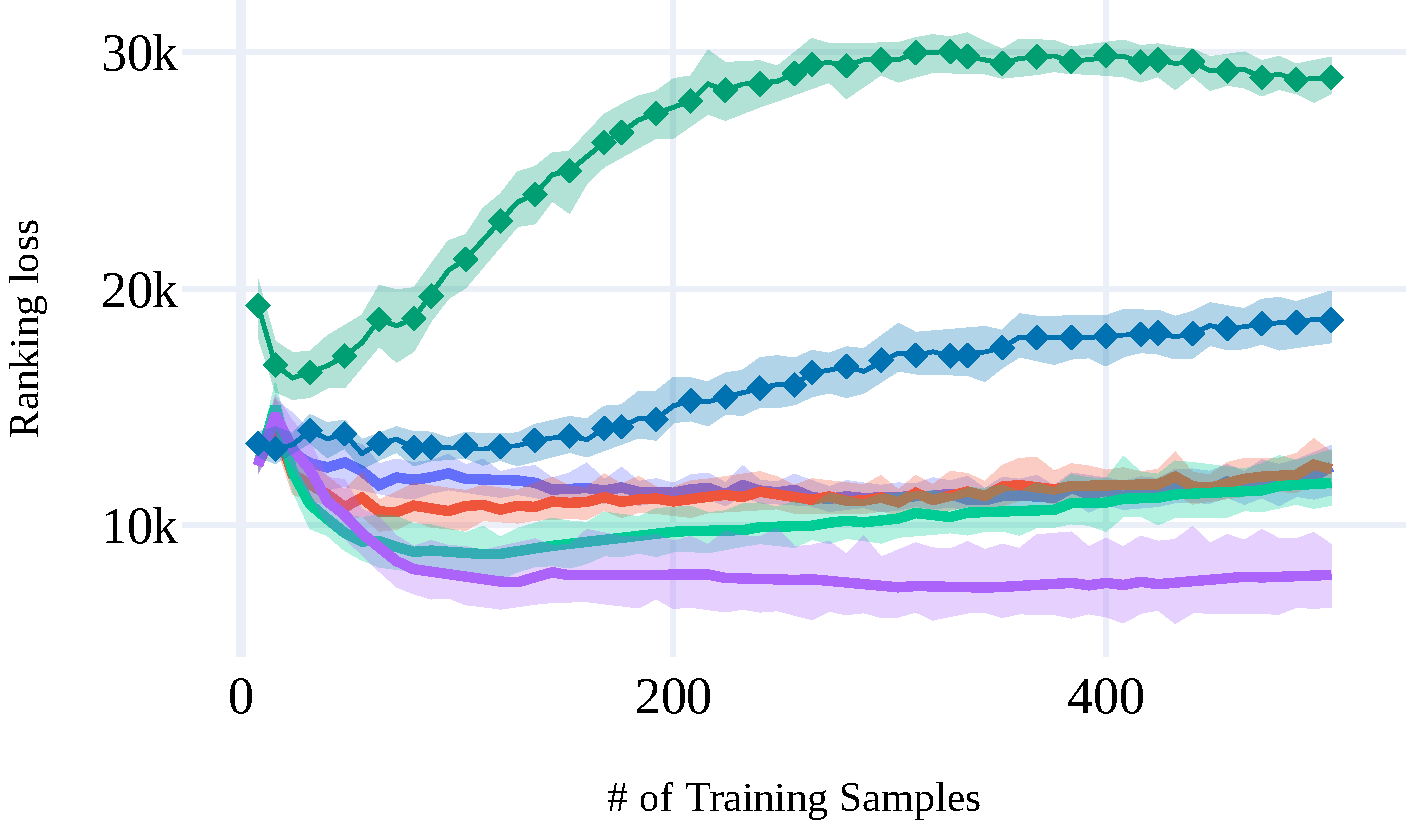
\includegraphics[scale=0.33]{figures/05/figs/figs/model_acc.pdf}
        \caption{All}
    \end{subfigure}
    \begin{subfigure}{0.49\textwidth}
        \centering
        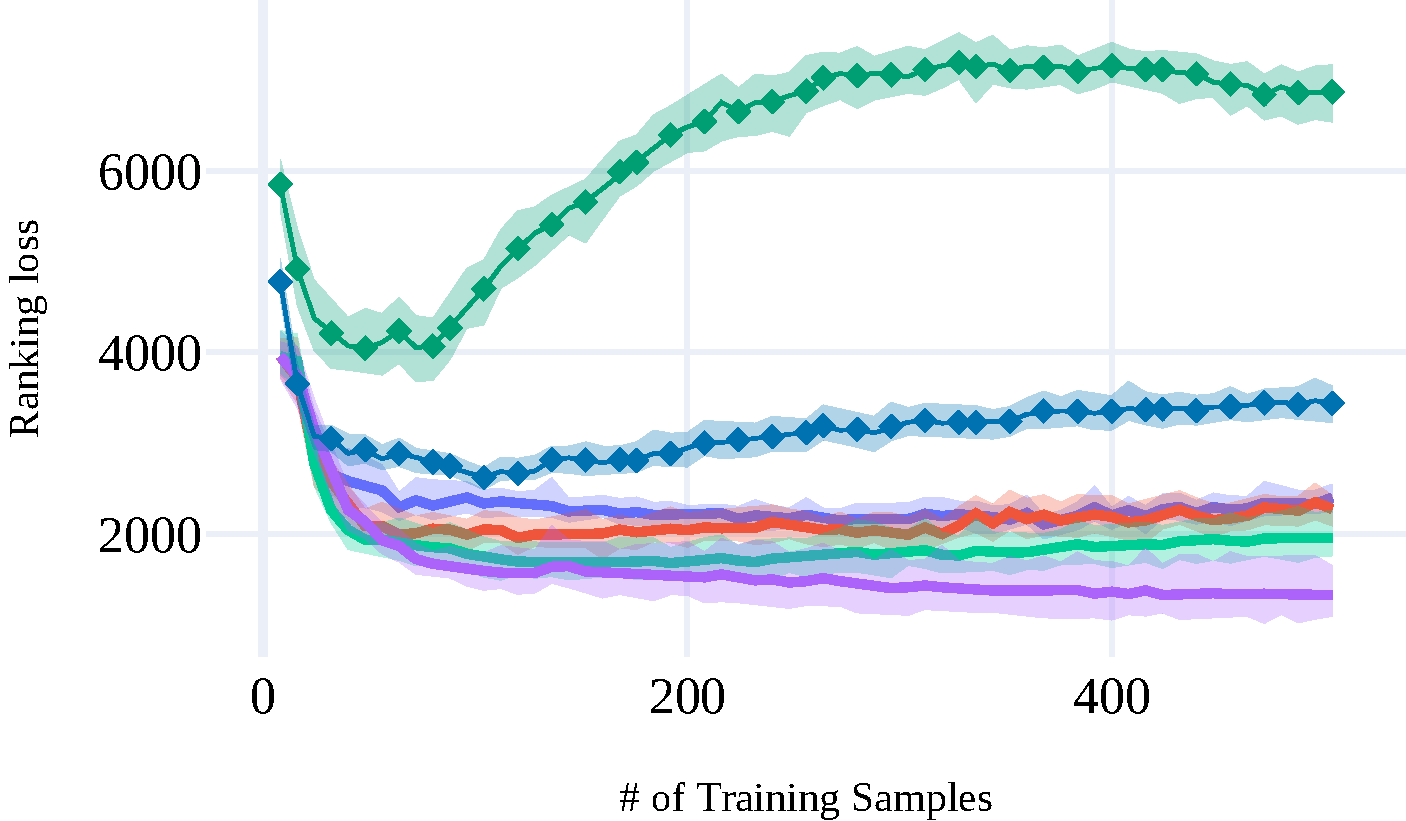
\includegraphics[scale=0.33]{figures/05/figs/figs/model_acc_best50.pdf}
        \caption{Top 50\%}
    \end{subfigure}
    \begin{subfigure}{0.49\textwidth}
        \centering
        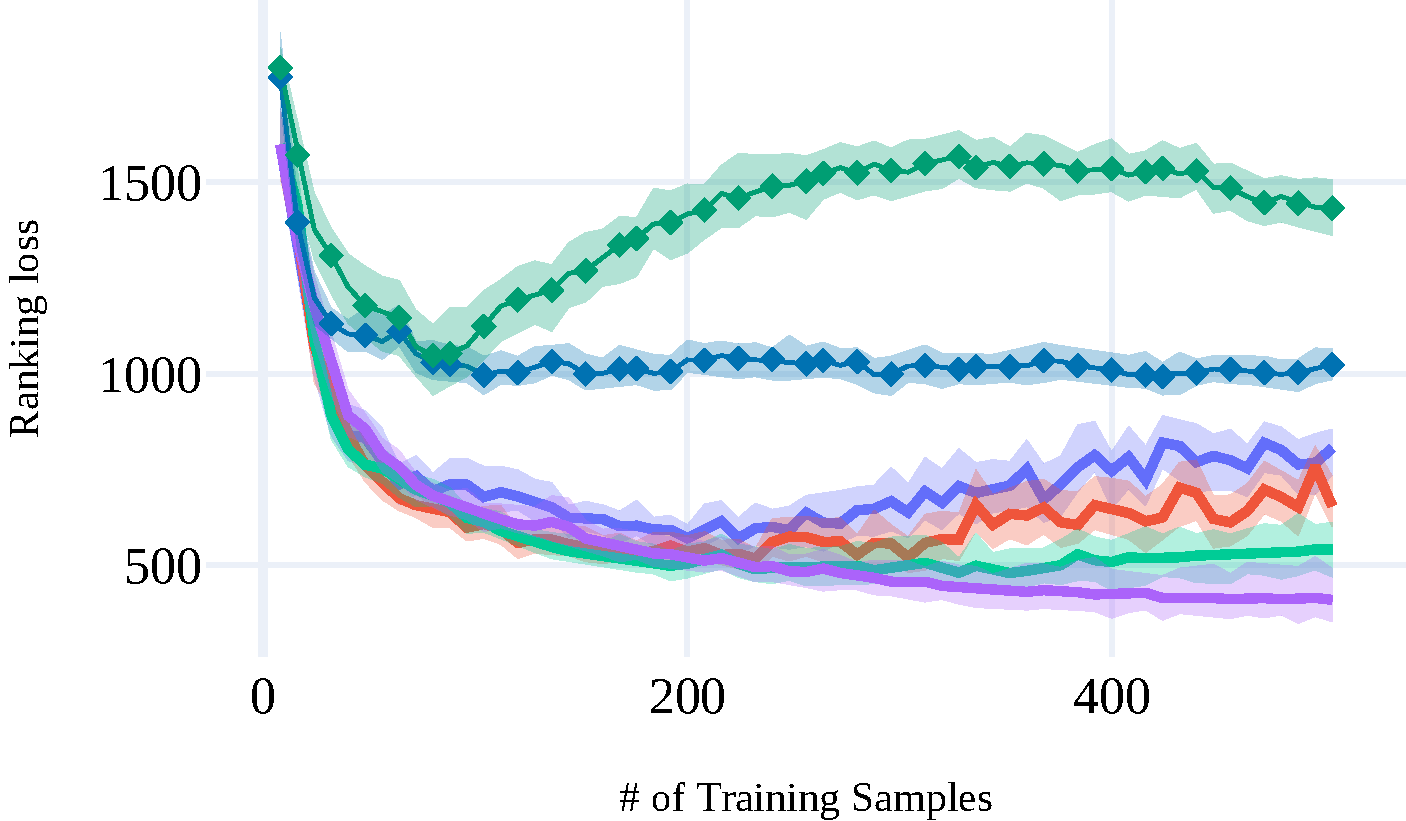
\includegraphics[scale=0.33]{figures/05/figs/figs/model_acc_best25.pdf}
        \caption{Top 25\%}
    \end{subfigure}
    \begin{subfigure}{0.49\textwidth}
        \centering
        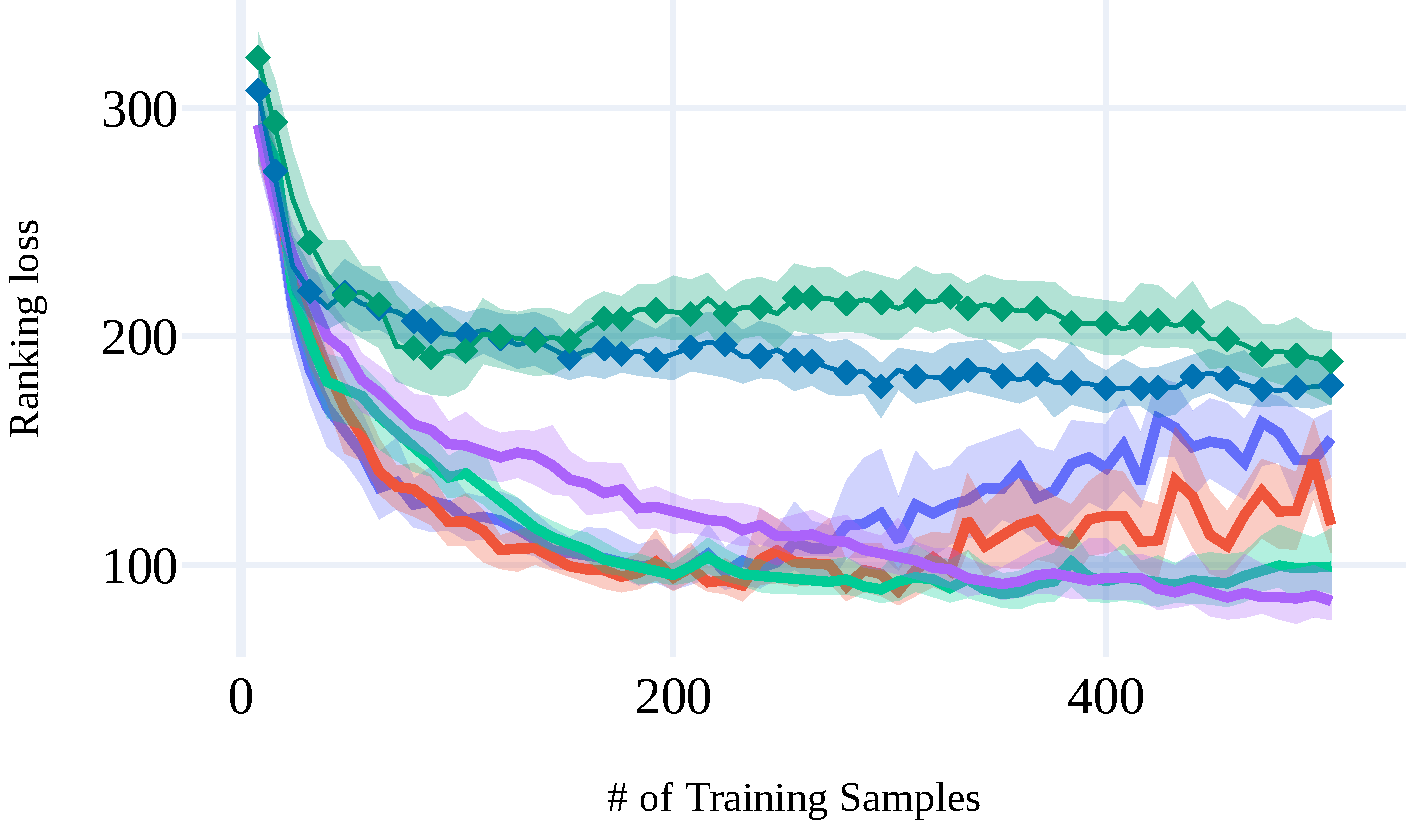
\includegraphics[scale=0.33]{figures/05/figs/figs/model_acc_best10.pdf}
        \caption{Top 10\%}
    \end{subfigure}
    
    
\includegraphics[scale=0.33]{figures/05/figs/figs/model_acc_legend.pdf}
    \caption{Ranking loss as a measure of surrogate accuracy of \texttt{DyMBO} (with different values of $\alpha$) and single-surrogate HEBO variants with RF and GP. The ranking loss is measured on randomly sampled configurations: (a) ranking on all configurations; (b) ranking on the top 50\% of configurations; (c) ranking on the top 25\% of configurations; and (d) ranking on the top 10\% of configurations. All \texttt{DyMBO} variants exhibit substantially better ranking loss than single-surrogate baselines. 
    }
    \label{fig:ch05:surrogate-accuracy}
\end{figure}



\section{Additional baselines}
\label{sec:ch05:add_baselines}

We describe additional baselines against which we compared our method. We note that these baselines are described in the appendix and not in the main paper as they are either not an established HPO method or not compatible with some of the benchmarks.

\paragraph{HEBO with different surrogate models.} To isolate the effect of the surrogate model, we evaluated four single-surrogate HEBO variants using GP, RF, ET, and GB, respectively. All other components of the optimisation pipeline, including the initial-design strategy, acquisition function, and acquisition-function optimiser, were kept unchanged. \cref{fig:ch05:gen_res_more_surrogate} compares these variants with \texttt{DyMBO} ($\alpha=1.0$) and random search. The relative performance of the single-surrogate variants varies with the cost of the target function: GP performs particularly well on cheap and medium-cost functions, whereas RF becomes the strongest single-surrogate baseline on expensive functions toward the end of the optimisation. ET and GB generally obtain lower ranks, although their relative performance also changes across budget groups. \texttt{DyMBO} achieves the best mean rank in every group, demonstrating the benefit of dynamically selecting between complementary surrogate models instead of committing to a single model before optimisation.

\begin{figure*}[h]
    \centering
    \begin{subfigure}[t]{0.49\textwidth}
        \centering
        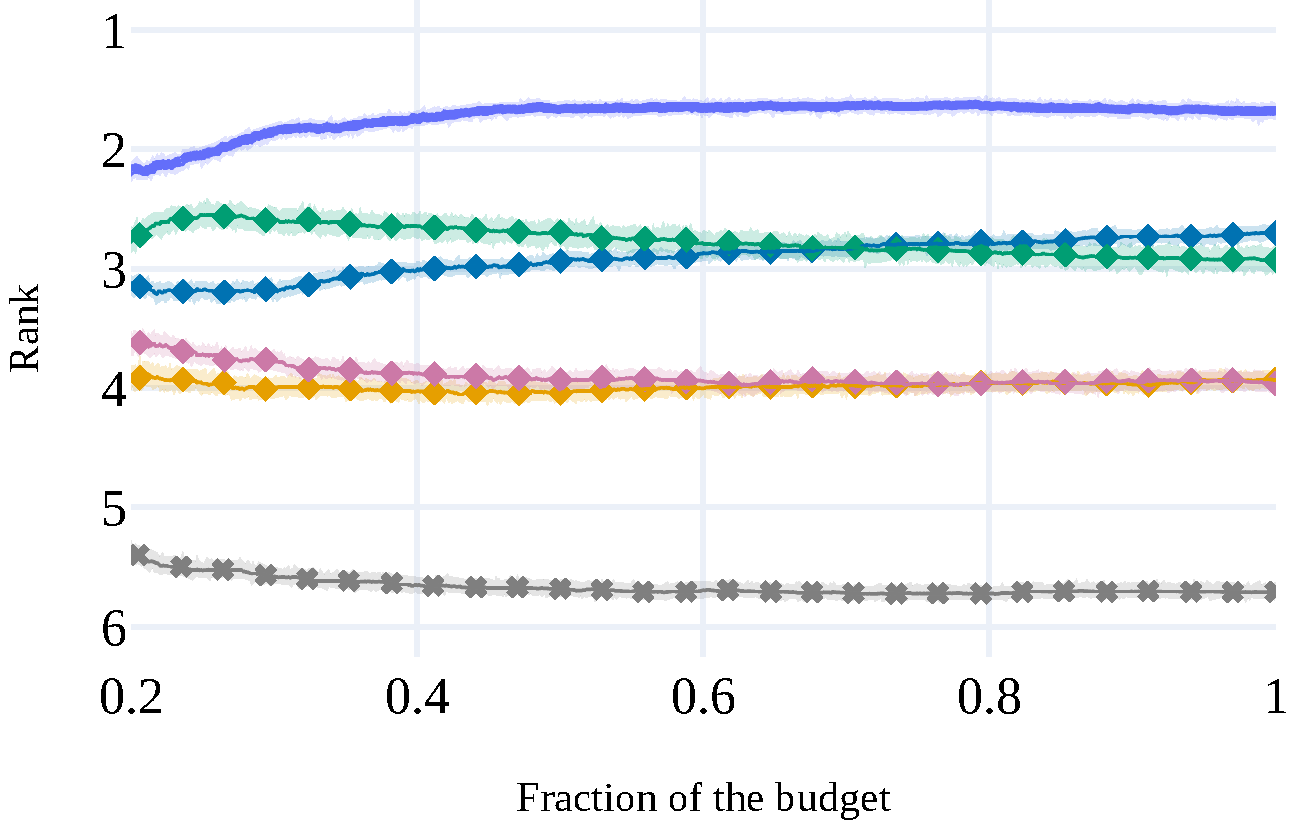
\includegraphics[scale=0.33]{figures/05/figs/figs/ranks/main_ranks_all_surrogates2_all.pdf}
        \caption{All target functions}
    \end{subfigure}
    \begin{subfigure}[t]{0.49\textwidth}
        \centering
        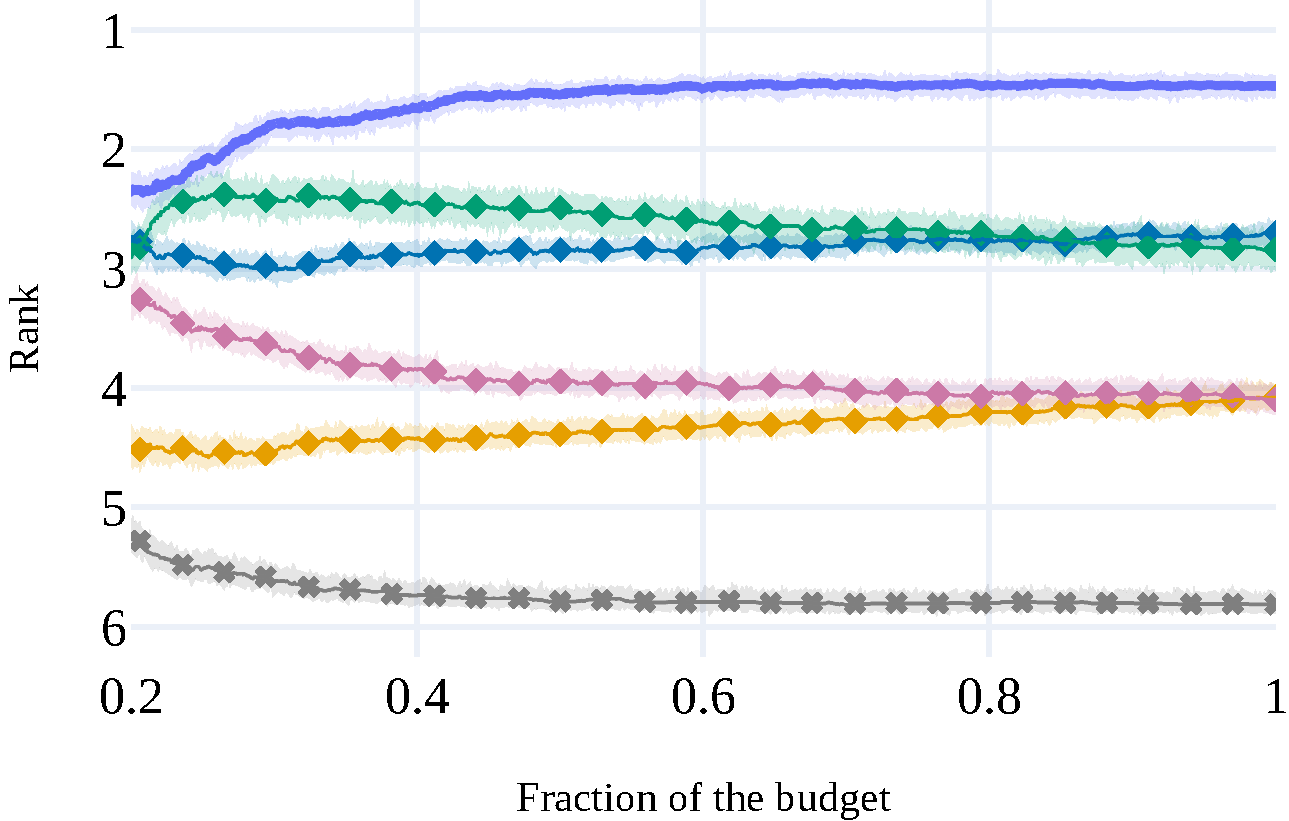
\includegraphics[scale=0.33]{figures/05/figs/figs/ranks/main_ranks_all_surrogates2_cheap.pdf}
        \caption{Cheap (up to 10 minutes)}
    \end{subfigure}
    \begin{subfigure}[t]{0.49\textwidth}
        \centering
        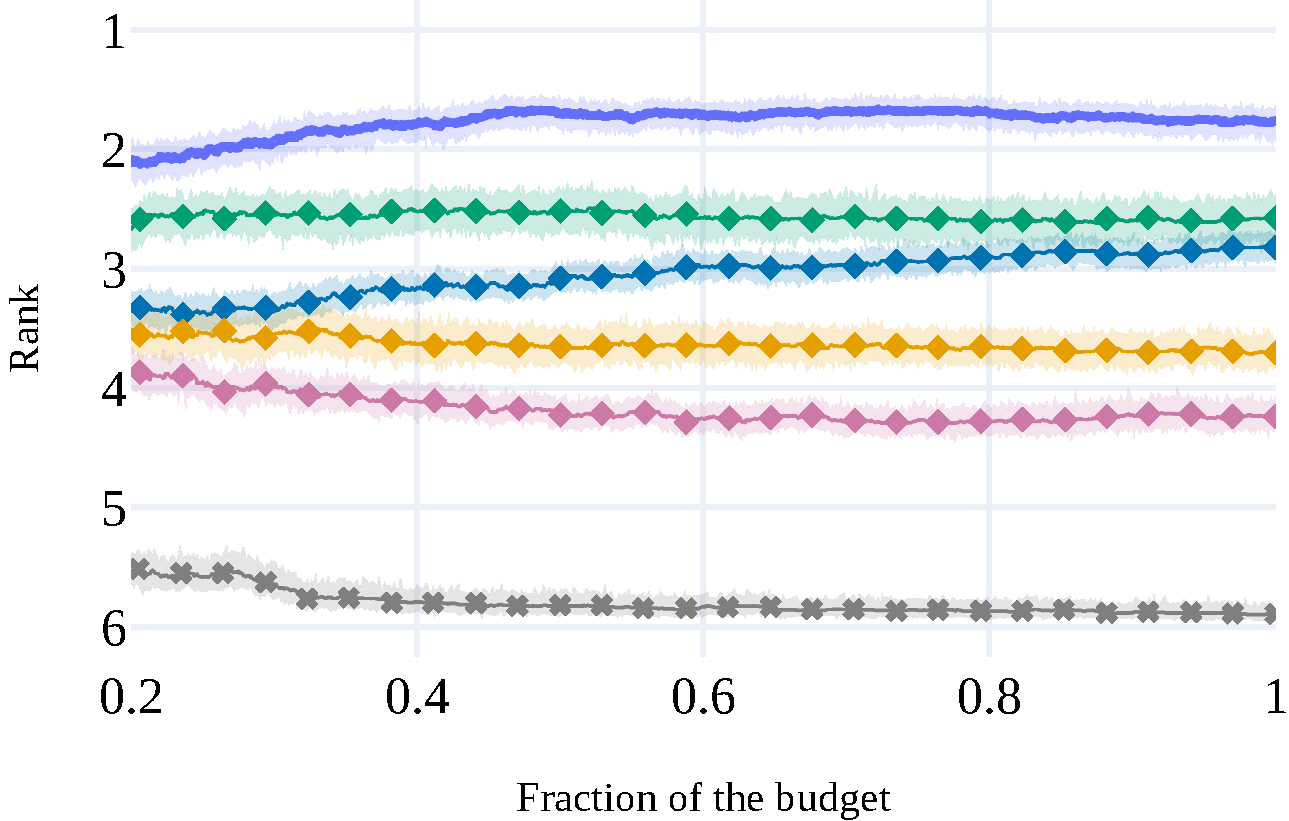
\includegraphics[scale=0.33]{figures/05/figs/figs/ranks/main_ranks_all_surrogates2_medium.pdf}
        \caption{Medium-cost (more than 10 minutes, up to \mbox{1 hour})}
    \end{subfigure}
    \begin{subfigure}[t]{0.49\textwidth}
        \centering
        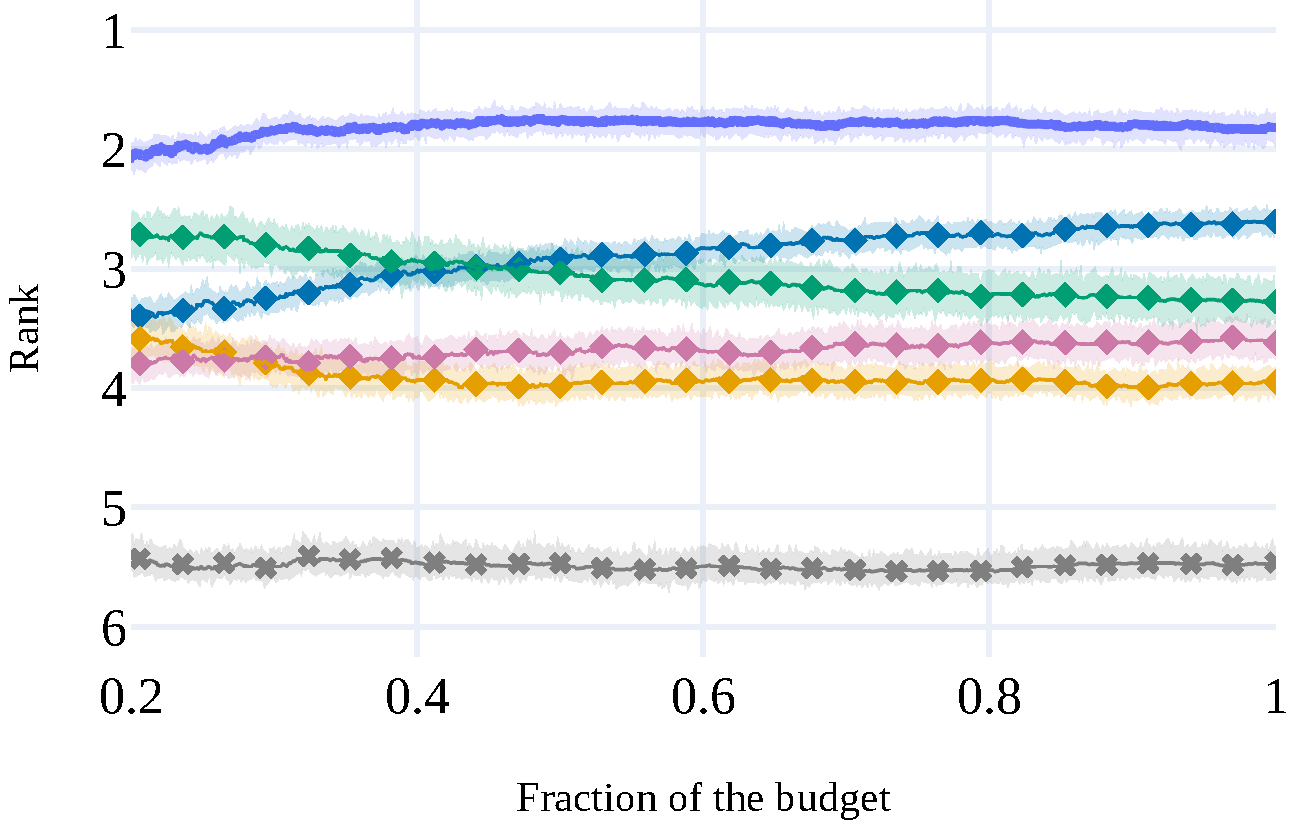
\includegraphics[scale=0.33]{figures/05/figs/figs/ranks/main_ranks_all_surrogates2_expensive.pdf}
        \caption{Expensive (more than 1 hour)}
    \end{subfigure}
    \begin{subfigure}[t]{\textwidth}
        \centering
        
\includegraphics[scale=0.33]{figures/05/figs/figs/ranks/main_ranks_all_surrogates2_all_legend.pdf}
    \end{subfigure}
    \caption{
    Mean rank of DyMBO with $\alpha=1.0$, single-surrogate HEBO variants using RF, GP, ET, or GB, and random search on YAHPO Gym and JAHS-Bench-201 as a function of the fraction of the wall-clock time budget for each task. Results are shown for (a) all target functions, (b) cheap functions with budgets of up to 10 minutes, (c) medium-cost functions with budgets between 10 minutes and 1 hour, and (d) expensive functions with budgets exceeding 1 hour. Smaller numbers indicate a better rank, thus better performance. \texttt{DyMBO} achieves the best mean rank in every budget group, while the relative performance of the individual surrogate models varies with target function cost.
    }
    \label{fig:ch05:gen_res_more_surrogate}
\end{figure*}

\paragraph{Squirrel.}
Squirrel~\citep{AwaEtAl20} is an HPO method which won the third place in the NeurIPS black-box optimisation challenge. 
Squirrel uses a GP surrogate model and a portfolio of acquisition functions, including EI, PI, Lower Confidence Bound (LCB)~\citep{ForEtAl08} and logEI~\citep{HutEtAl11}, selected adaptively during optimisation.
It should be noted that Squirrel was specifically designed to meet the rules of the challenge (batch size, number of random samples, total number of batches). A similar approach is Optuna AutoSampler, which selects the HPO method to use based on hand-crafted rules. We ran Squirrel only on the YAHPO Gym benchmark, as it is not compatible with JAHS-Bench-201 due to Python package versioning. We provide the results in \cref{fig:ch05:squirrel}, where we see that our approach outperforms Squirrel on almost all benchmarks (mean rank of 1.07).


\begin{figure*}
    \centering
    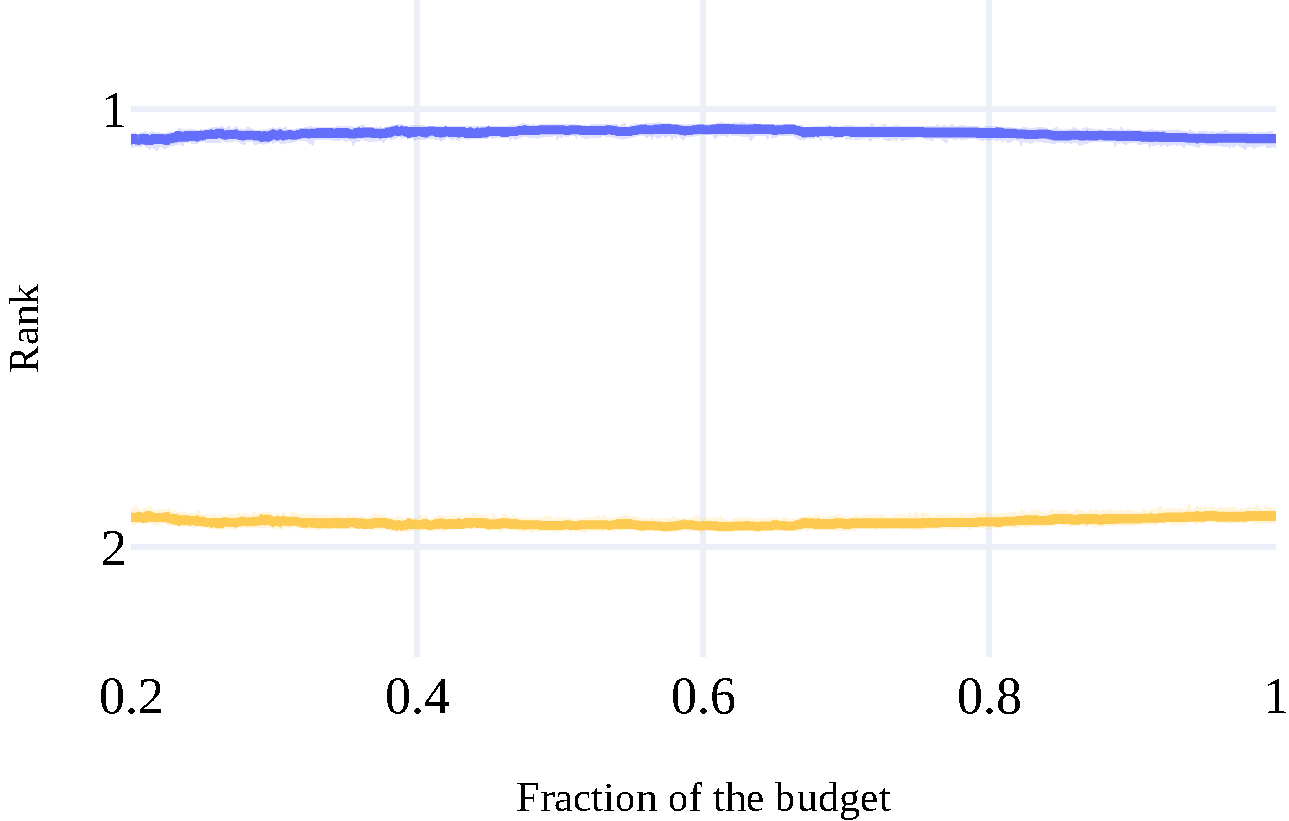
\includegraphics[scale=0.33]{figures/05/figs/figs/ranks/additional_baselines_squirrel_all.pdf}
    
\includegraphics[scale=0.33]{figures/05/figs/figs/ranks/additional_baselines_squirrel_all_legend.pdf}
    \caption{Comparison of \texttt{DyMBO} to Squirrel as a function of the fraction of the wall-clock time budget on YAHPO Gym. Our method outperforms Squirrel on almost all benchmarks. 
    }
    \label{fig:ch05:squirrel}

\end{figure*}

\begin{figure*}
    \centering
    \begin{subfigure}[t]{\textwidth}
    \centering
    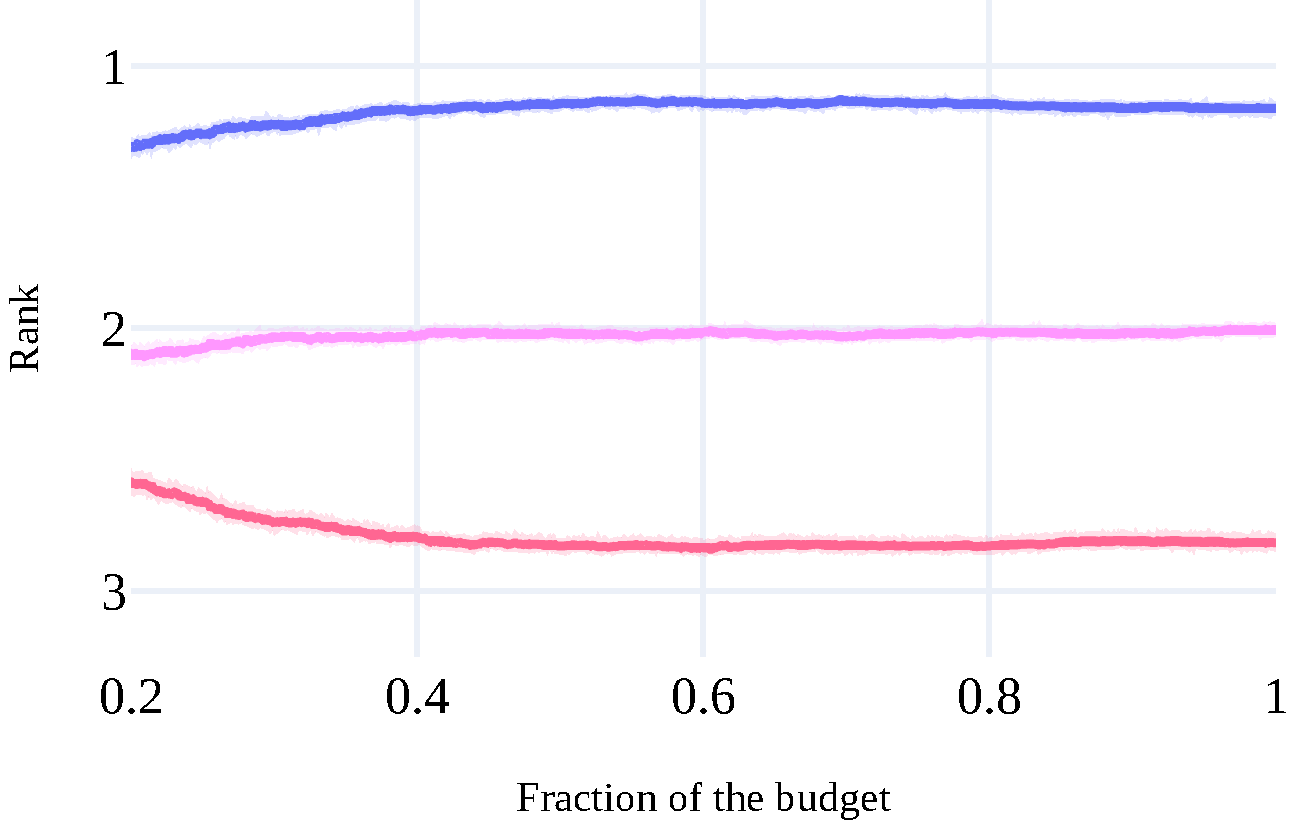
\includegraphics[scale=0.33]{figures/05/figs/figs/ranks/additional_baselines_all.pdf}
    \end{subfigure}
    
\includegraphics[scale=0.33]{figures/05/figs/figs/ranks/additional_baselines_all_legend.pdf}
    \caption{Comparison of \texttt{DyMBO} to simple selection and equal weights baselines as a function of the fraction of the wall-clock time budget on YAHPO Gym and JAHS-Bench-201. Our method outperforms both baselines.
    % \todo{missing line in te label}
    }
    \label{fig:ch05:add_baselines}

\end{figure*}


\paragraph{Selection of the best surrogate and equal weights.}
We compared our method to two additional baselines: one that simply averages the predictions of the surrogate models (RF and GP), and a simple selection baseline, which selects the best performing (\emph{i.e.}, most accurate) surrogate model after the initial 8 samples and uses only this model for the rest of the optimisation. 
Since both baselines are HEBO-based, they inherit MACE as the acquisition function.
We performed the selection using 8-fold cross-validation, and we used the MSE loss as an accuracy metric; we then chose the surrogate which yields the most accurate predictions. 
We provide the results in~\cref{fig:ch05:add_baselines}, where we see that our method outperforms both baselines. This emphasises the effectiveness of dynamically assigning weights to the surrogate models.

\paragraph{Random selection of surrogates.}
Finally, we compared our method to another simple selection baseline that chooses a surrogate uniformly at random in each iteration.
In this experiment, we used RF and GP as surrogate models with 8 initial samples.
% \changed{
\cref{fig:ch05:rnd_sel_rnk} shows that \texttt{DyMBO} maintains a substantially better mean rank throughout the optimisation. To further analyse this, we present in~\cref{fig:ch05:rnd_sel_ecdf} a task-level comparison of the final objective values, where we compare the log-scaled ratio between the final values \texttt{DyMBO} achieved and the final values that the random selection baseline achieved. Positive log-ratios show that \texttt{DyMBO} performs better, negative values show that random selection perform better, and zero indicates equal performance. \texttt{DyMBO} obtains a better final value on 406 of the 859 tasks, while random selection performs better on 262 tasks, and the two methods are tied on the remaining 191 tasks. These results indicate that the gains of \texttt{DyMBO} cannot be explained solely by randomly switching between complementary surrogate models, as selecting the surrogate according to its observed ranking accuracy provides a clear advantage over random switching.
% }


\begin{figure}
    \centering
    \begin{subfigure}[t]{0.49\textwidth}
        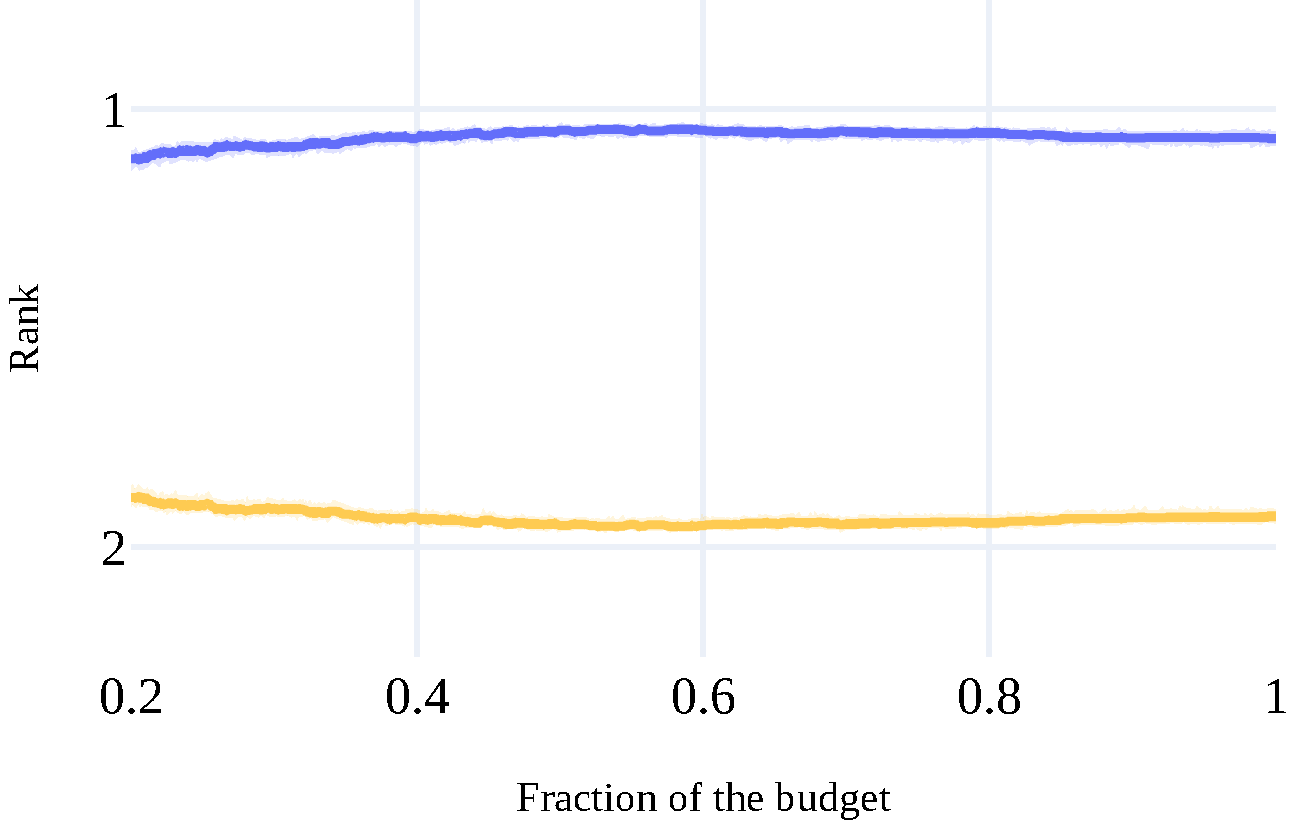
\includegraphics[scale=0.33]{figures/05/figs/figs/ranks/comp_rnd_choice2_all.pdf}
        \caption{}
        \label{fig:ch05:rnd_sel_rnk}
    \end{subfigure}
    
    \begin{subfigure}[t]{0.49\textwidth}
        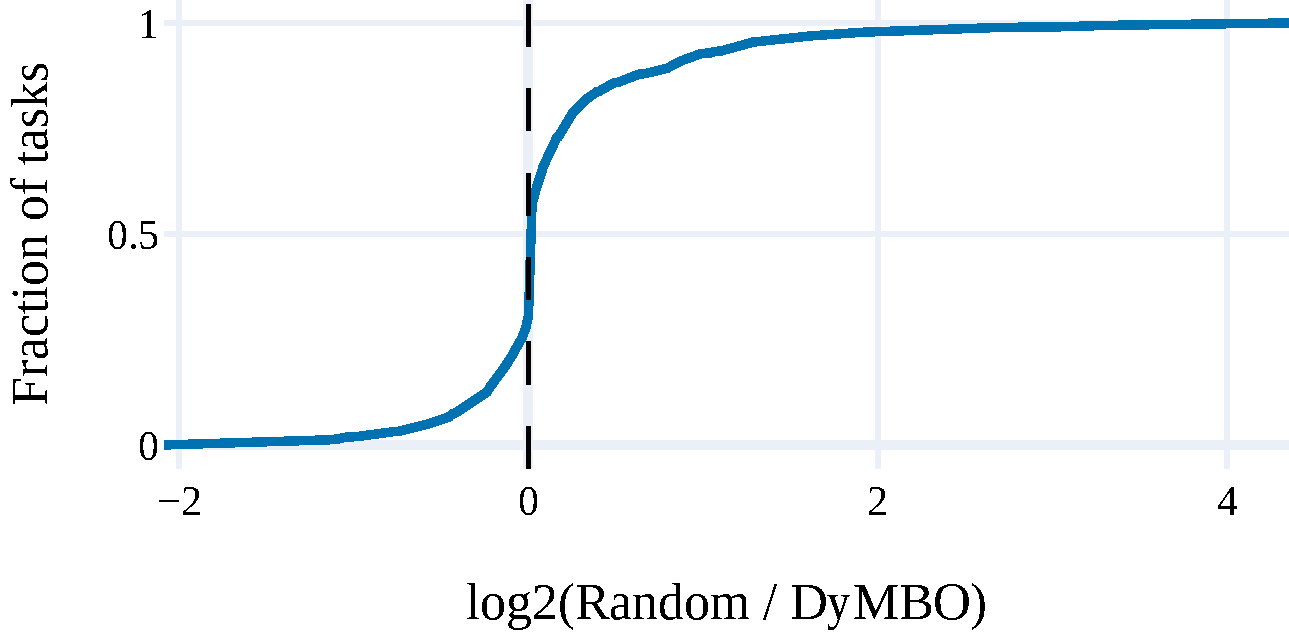
\includegraphics[scale=0.33]{figures/05/figs/figs/ranks/comp_rnd_choice_final_regret_log_ratio_ecdf.pdf}
        \caption{}
        \label{fig:ch05:rnd_sel_ecdf}
    \end{subfigure}
    
\includegraphics[scale=0.33]{figures/05/figs/figs/ranks/comp_rnd_choice2_all_legend.pdf}
    \caption{Comparison of \texttt{DyMBO} with $\alpha=1.0$ against a baseline that randomly selects between the RF and GP surrogates at every iteration, evaluated on YAHPO Gym and JAHS-Bench-201. (a) Mean rank as a function of the fraction of  wall-clock time budget for each task; lower ranks indicate better performance. (b) Empirical cumulative distribution (ECDF) across tasks of the log-ratio between the final objective values obtained by random selection and \texttt{DyMBO}. Positive values favour \texttt{DyMBO}, negative values favour random selection, and zero indicates equal performance. \texttt{DyMBO} performs better on 406 of the 859 tasks, random selection performs better on 262 tasks, and the remaining 191 tasks are tied.
    }
    \label{fig:ch05:random-surrogates}
\end{figure}


\section{Different setups of experiments}
\label{sec:ch05:diff_exp_setup}

We ran \texttt{DyMBO} with different setups of experiments in addition to the one corresponding to the main results from~\cref{sec:ch05:res_general}. We first explore the effects of using a fixed number of evaluations, as compared to a time-based budget. We then investigate the performance of our method with a varying size of initial design, \emph{i.e.}, for different numbers of initial random samples. 
We also look into whether different batch sizes affect the performance of \texttt{DyMBO}.

\paragraph{Fixed number of evaluations.}
\label{sec:ch05:256_evals}

In addition to the main results in~\cref{sec:ch05:res_general}, we performed additional experiments to assess the effectiveness of our method as a function of the number of evaluations and not as the budget measured in wall-clock time. 
We used 8 initial samples and a total budget of 512 evaluations. 
This additional experiment was designed to show the ability of the optimiser to find good-performing candidates, regardless of the running time required for the optimiser or the target function. 
We evaluated the approach on YAHPO Gym, and the results are presented in~\cref{fig:ch05:ranks512}.
We see that \texttt{DyMBO} outranks the single-surrogate baselines when budget is measured in terms of the number of function evaluations.
% Dynamic ensembling is ranked better, with $\alpha=0.9$ having the best performance, closely followed by $\alpha=1.0$. 
% All dynamic ensembling methods are ranked better than the single surrogate baselines, as well as the static ensemble with equal weights to all models.

\begin{figure}
    \centering
    % \begin{subfigure}[t]{0.49\textwidth}
        % \centering
    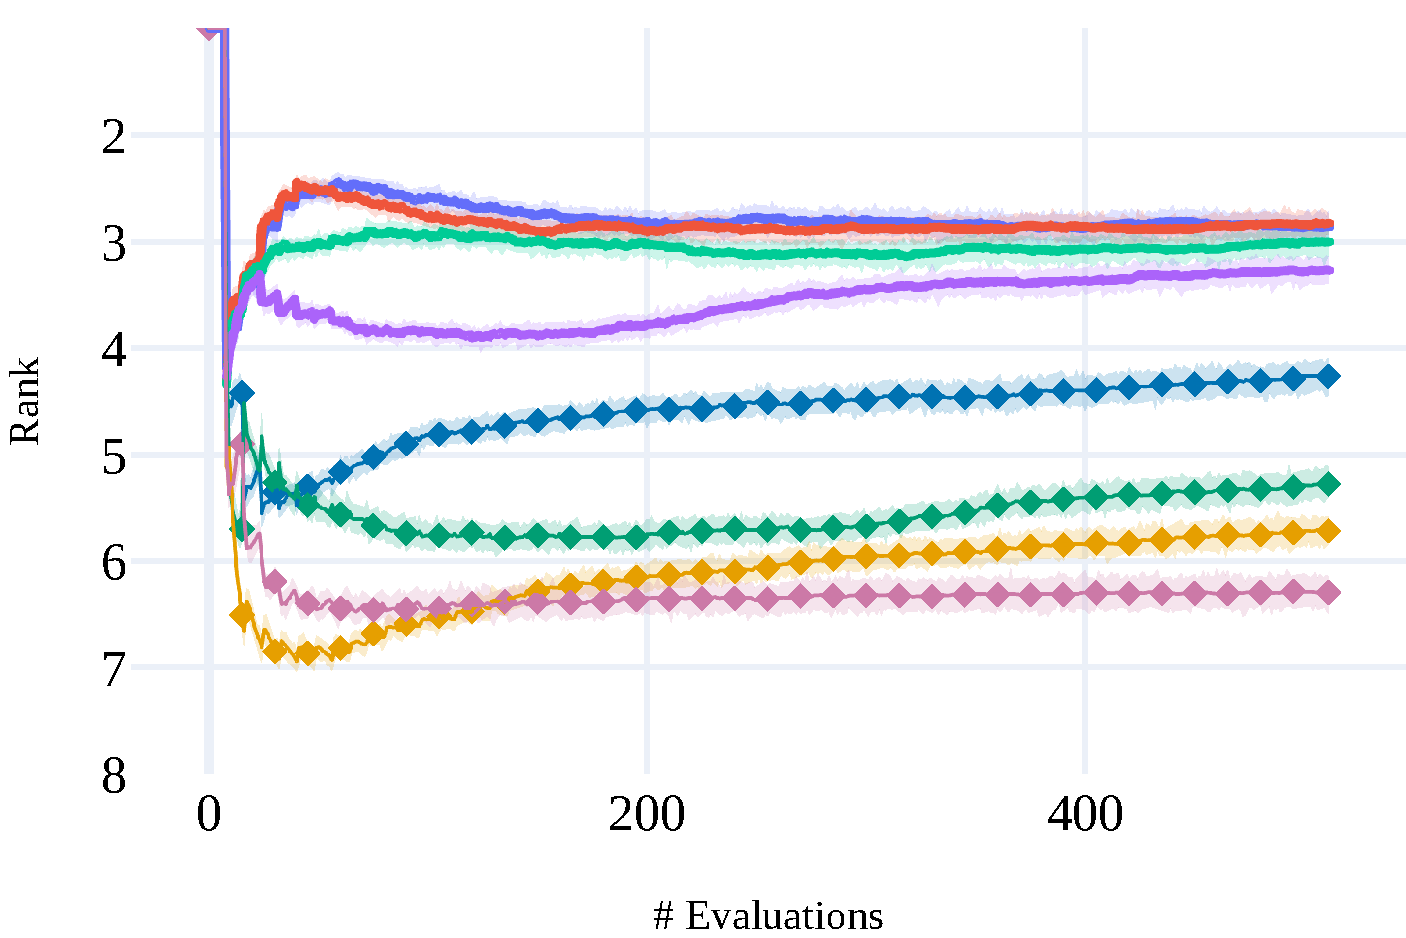
\includegraphics[scale=0.33]{figures/05/figs/figs/ranks/main_ranks_all_fixed.pdf}
    % \end{subfigure}
    % \begin{subfigure}[t]{0.49\textwidth}
    %     \centering
    %     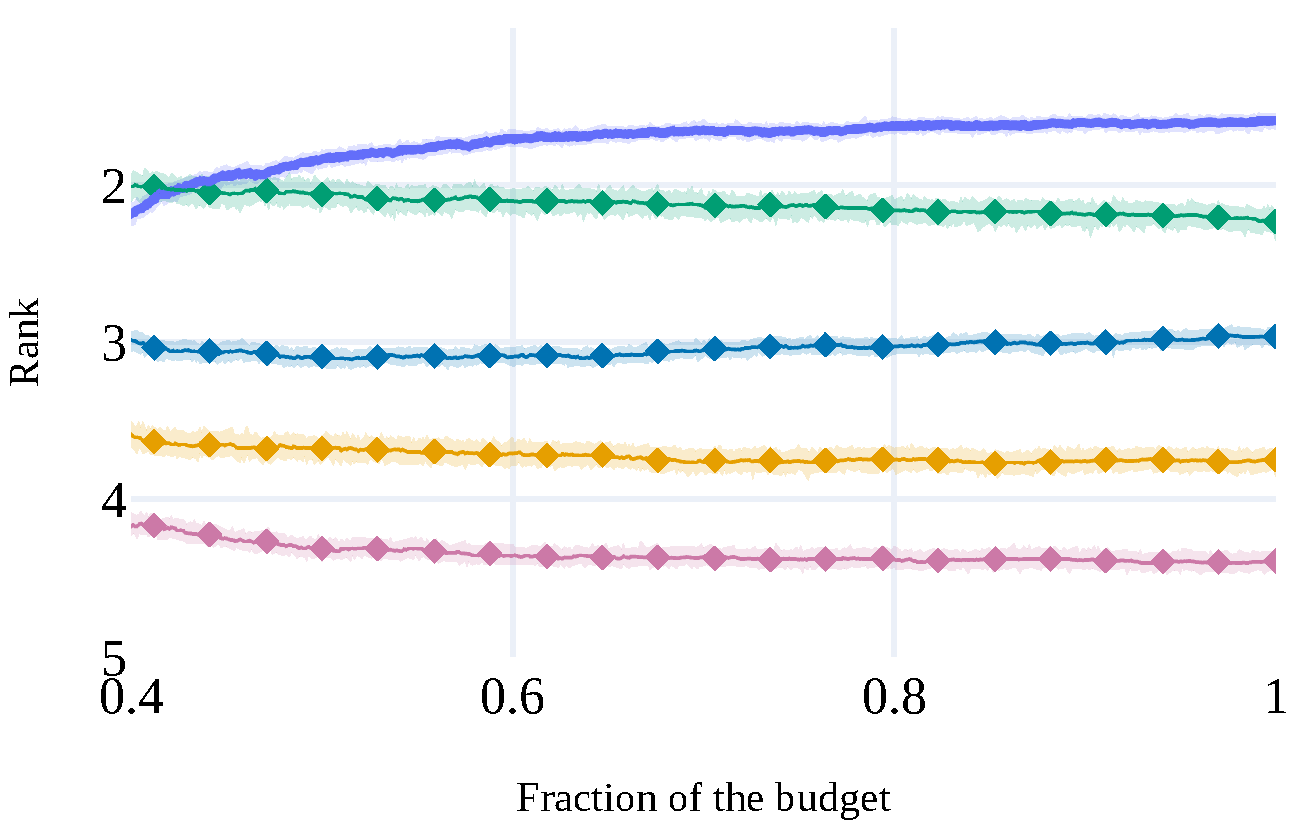
\includegraphics[scale=0.33]{figures/06/figs/figs/ranks/main_ranks_8_32_all.pdf}
    %     \caption{32}
    % \end{subfigure}
    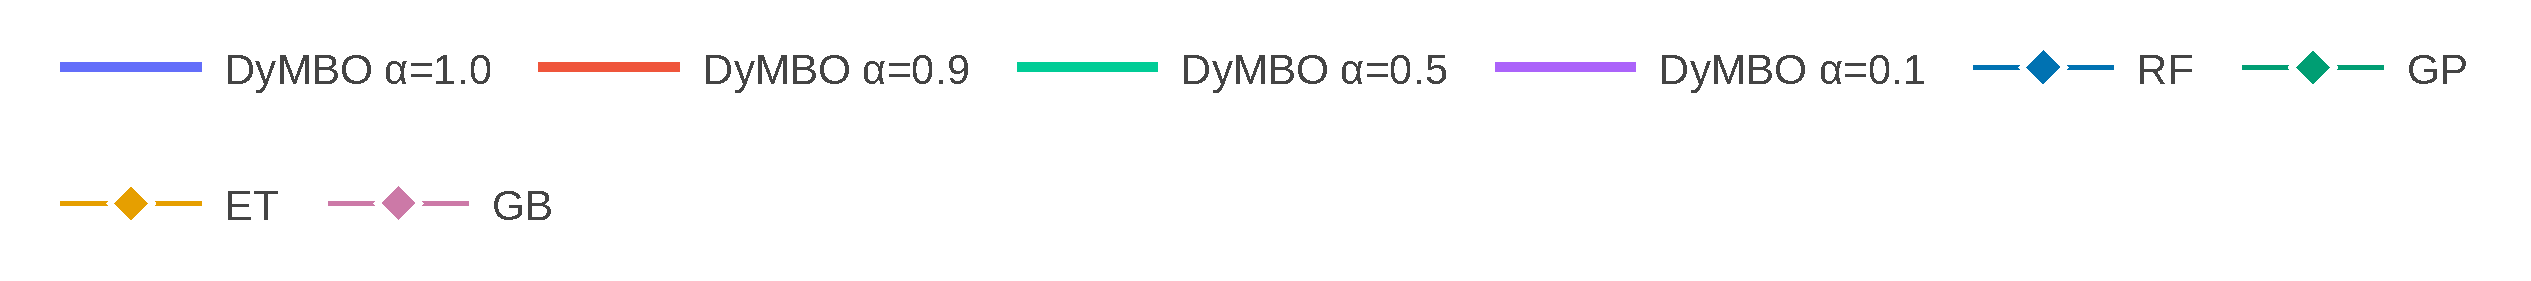
\includegraphics
    [scale=0.33]{figures/05/figs/figs/ranks/main_ranks_all_fixed_legend.pdf}
    \caption{Mean ranks of the different methods on YAHPO Gym and JAHS-Bench-201 as a function of the number of evaluations, with a total budget of 512 evaluations. \texttt{DyMBO} exhibits the best performance.
    }
    \label{fig:ch05:ranks512}
\end{figure}


\paragraph{Different number of initial samples.}
\label{sec:ch05:diff_init_samp}
We evaluated the performance of our method with different numbers of initial random samples. We used 16 and 32 initial samples, in addition to the 8 initial samples in~\cref{sec:ch05:res_general}. We used a total budget of $100\times$ average evaluation time. We evaluated the method on YAHPO Gym and JAHS-Bench-201, and the results are presented in~\cref{fig:ch05:diff_init_samp}. We see that \texttt{DyMBO} outperforms the single-surrogate baselines in all cases.

\begin{figure}
    \centering
    \begin{subfigure}[t]{0.49\textwidth}
        \centering
        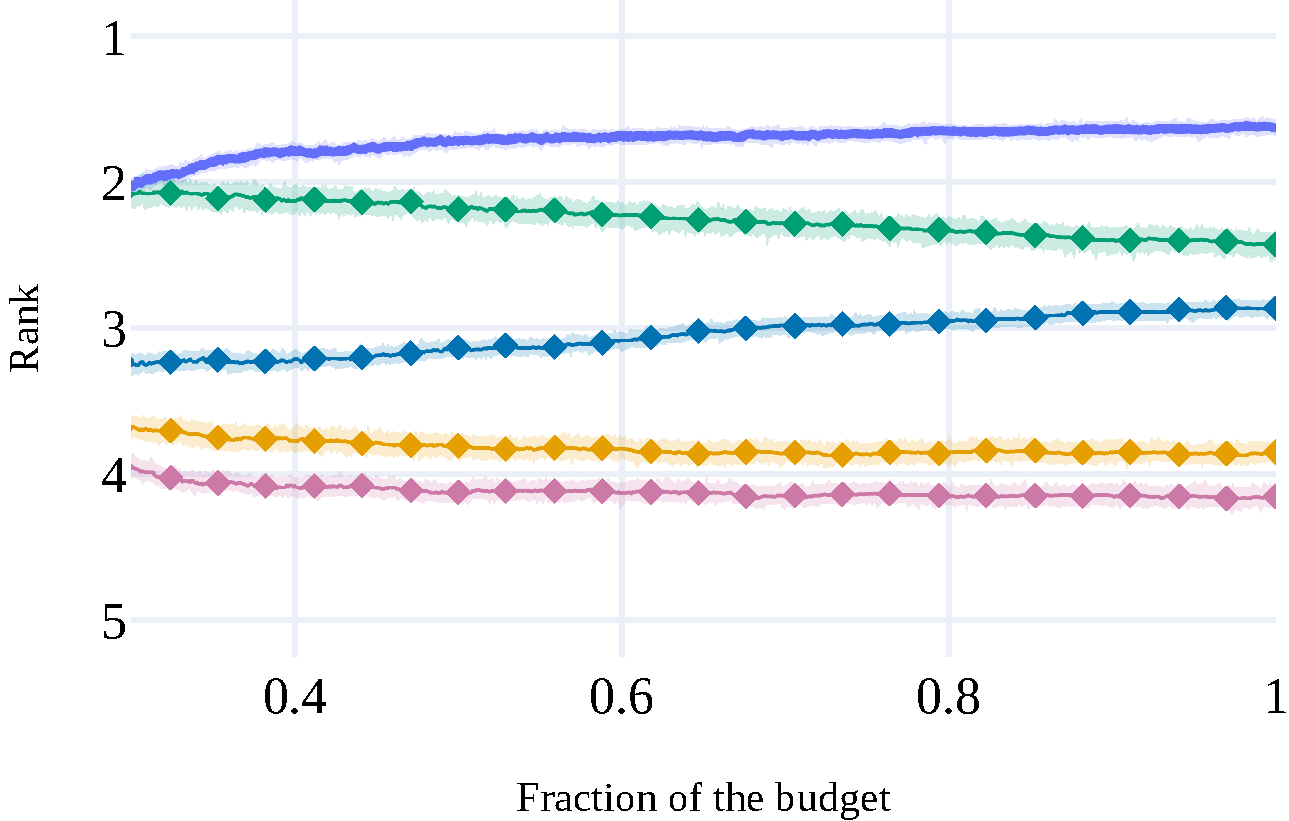
\includegraphics[scale=0.33]{figures/05/figs/figs/ranks/main_ranks_8_16_all.pdf}
        \caption{16 initial samples}
    \end{subfigure}
    \begin{subfigure}[t]{0.49\textwidth}
        \centering
        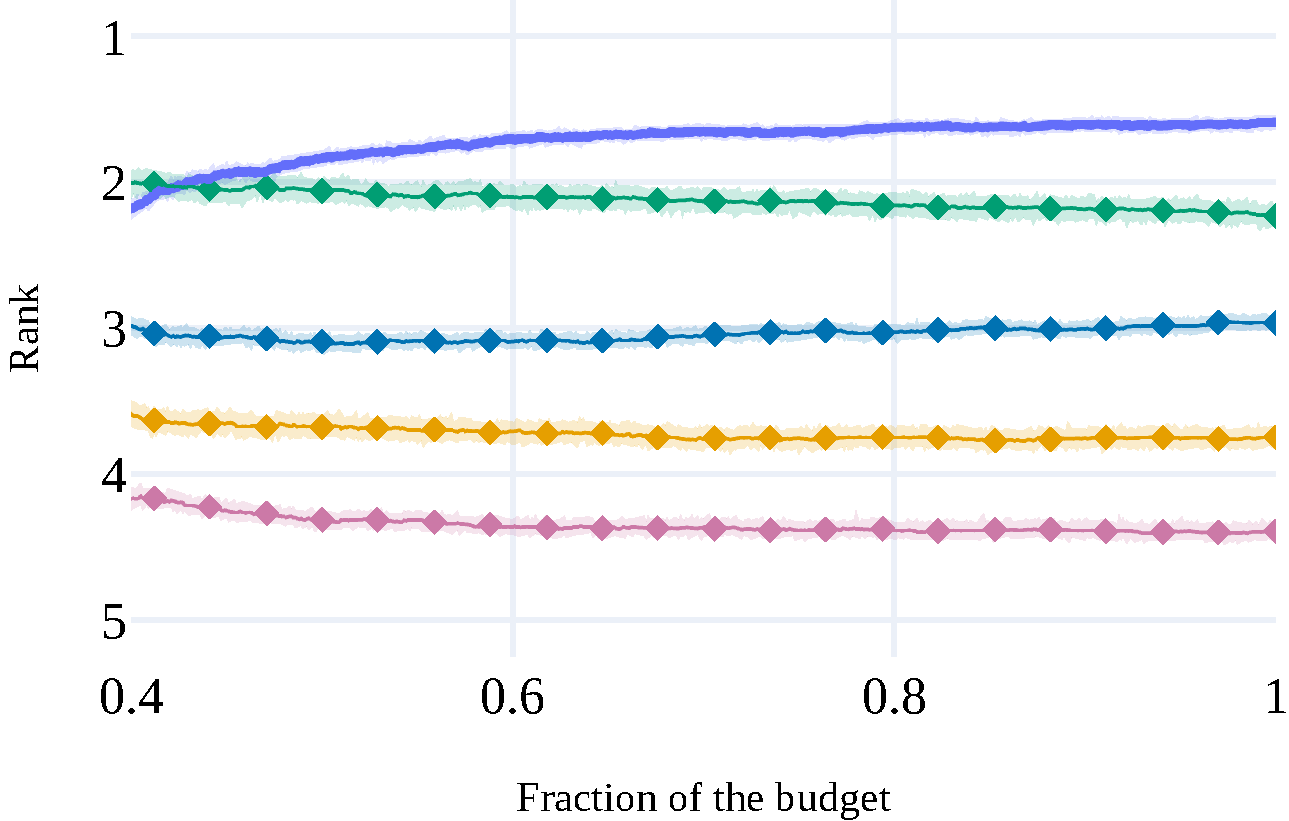
\includegraphics[scale=0.33]{figures/05/figs/figs/ranks/main_ranks_8_32_all.pdf}
        \caption{32 initial samples}
    \end{subfigure}
    \begin{subfigure}[t]{\textwidth}
        \centering
        
\includegraphics[scale=0.33]{figures/05/figs/figs/ranks/main_ranks_8_32_all_legend.pdf}
        % \caption{32 initial samples}
    \end{subfigure}
    
    \caption{Mean ranks with different numbers of initial samples as a function of the fraction of the wall-clock time budget on YAHPO Gym and JAHS-Bench-201. \texttt{DyMBO} achieves the best mean rank in both cases.
    % \todo{string "HEBO" can be dropped from the legends and explained in the caption, same for Fig.8 and Fig.9}
    }
    \label{fig:ch05:diff_init_samp}
\end{figure}

\paragraph{Different batch sizes.}
\label{sec:ch05:diff_batch_sizer}
We evaluated the performance of our method with different batch sizes. We used batch sizes of 1 (fully sequential sampling) and 4, in addition to the batch size of 8 in~\cref{sec:ch05:res_general}. For this experiment, we used a similar setup as in~\cref{sec:ch05:res_general}, with 8 initial samples and a total budget of $100\times$ average evaluation time. We evaluated the method on YAHPO Gym and JAHS-Bench-201, and the results are shown in~\cref{fig:ch05:diff_batch_sizer}. We see that with different batch sizes \texttt{DyMBO} also outperforms the single-surrogate baselines. We furthermore observe that RF performs better with batch sizes larger than 1, \emph{i.e.,} not in a fully sequential setup, based on both~\cref{fig:ch05:gen_res_simple,fig:ch05:diff_batch_sizer}.
% \aj{unresolved ref to fig}
% \er{Question: we say this only observing Figure 7, or also based on Figure 2, for batch size = 8?} \aj{We need to rephrase this a bit. For batch sizes 4 and 8 RF performs better than in a fully sequential setup. I don't see drastic differences in RF performance for batch 4 and batch 8.}

\begin{figure}
    \centering
    \begin{subfigure}[t]{0.49\textwidth}
        \centering
        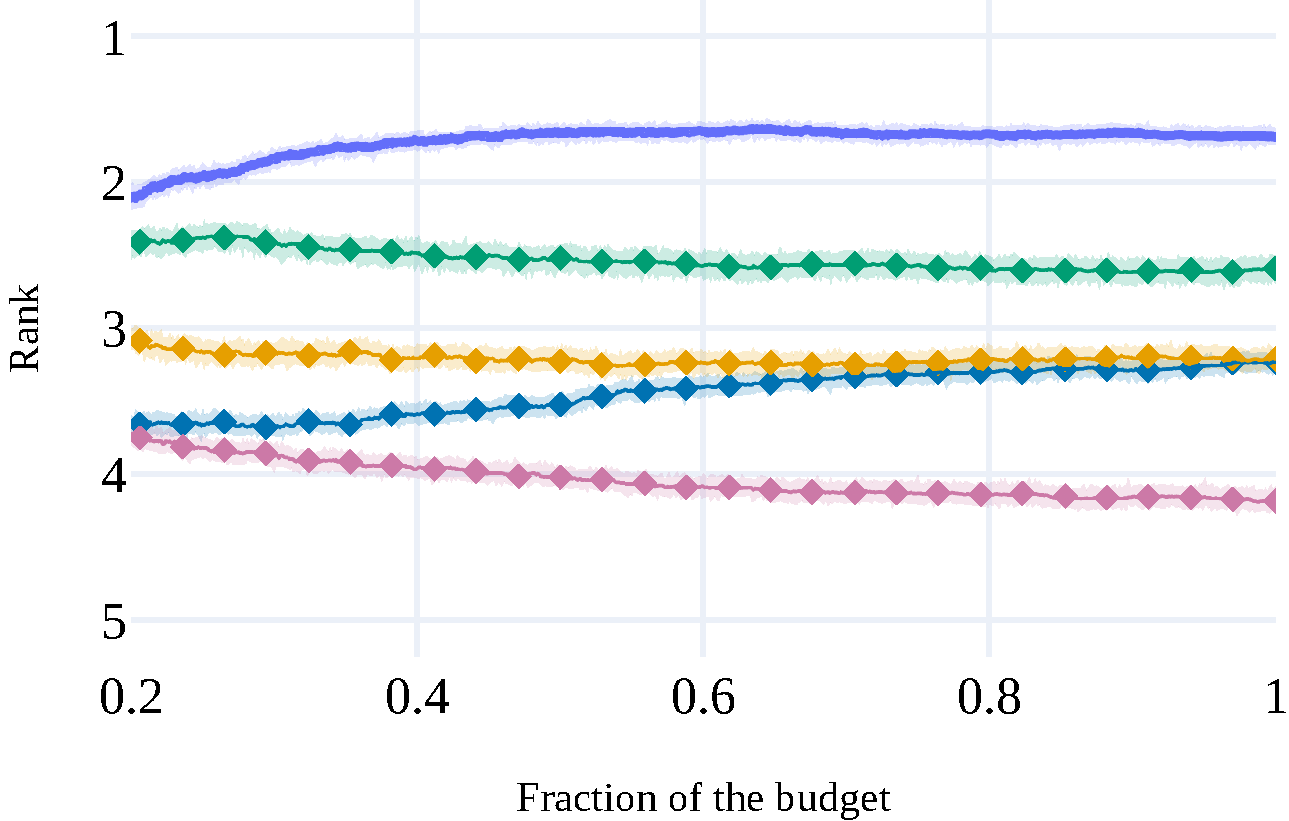
\includegraphics[width=\textwidth]{figures/05/figs/figs/ranks/main_ranks_1_8_all.pdf}
        \caption{Batch size 1 (fully sequential)}
    \end{subfigure}
    \begin{subfigure}[t]{0.49\textwidth}
        \centering
        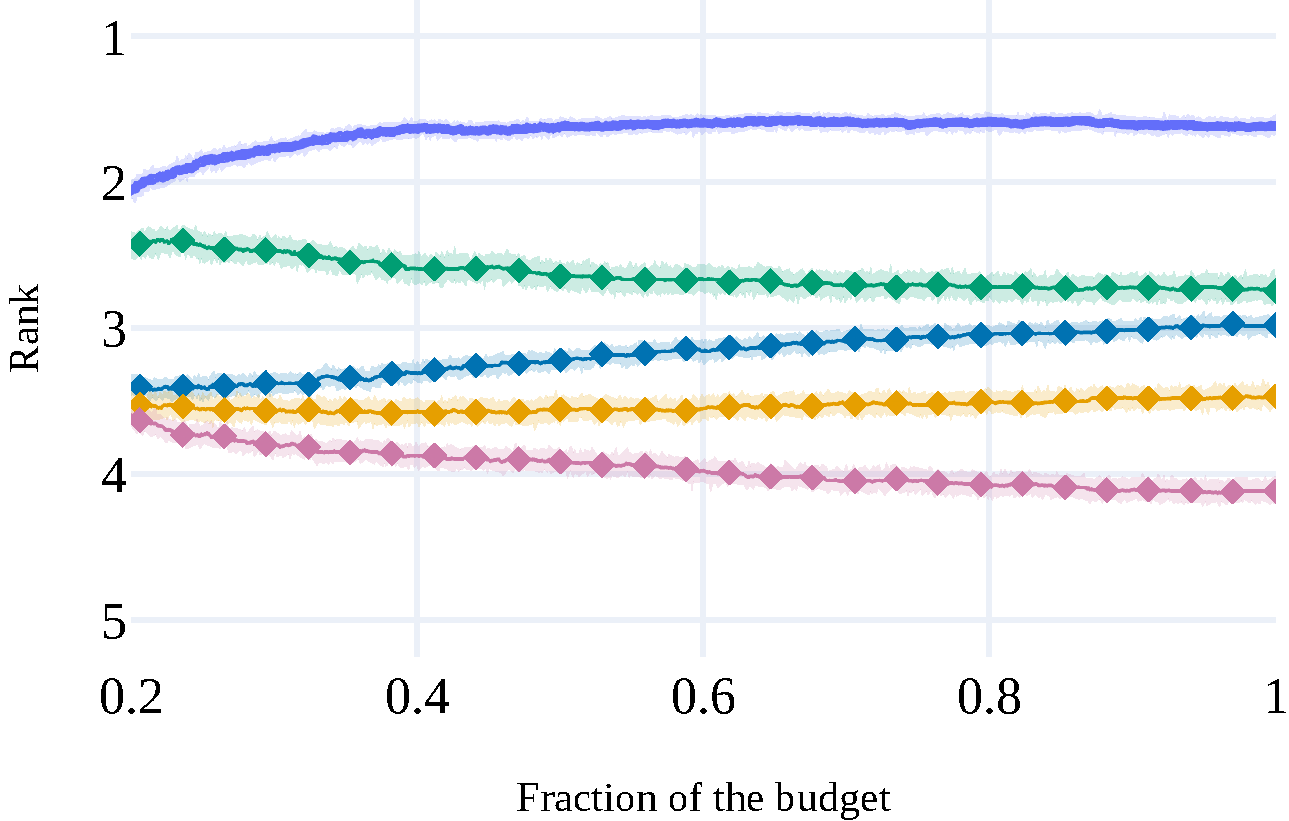
\includegraphics[width=\textwidth]{figures/05/figs/figs/ranks/main_ranks_4_8_all.pdf}
        \caption{Batch size 4}
    \end{subfigure}
    
\includegraphics[scale=0.33]{figures/05/figs/figs/ranks/main_ranks_4_8_all_legend.pdf}
    \caption{Mean ranks with different batch sizes as a function of the fraction of the wall-clock time budget on YAHPO Gym and JAHS-Bench-201. \texttt{DyMBO} has the best mean rank in both cases.
    % \todo{legend?}
    }
    \label{fig:ch05:diff_batch_sizer}
\end{figure}

\section{Ablation studies}
\label{sec:ch05:ablations}

% \er{Elena, readi this - new part (no H.3)} 
In this section, we describe several ablation studies we performed on our method. 
% In~\autoref{sec:app_alpha}, we first examine the effect of the value of the smoothing factor $\alpha$ of the exponential moving average for weight computation on the performance of \texttt{DyMBO}, \emph{i.e.}, how much the performance varies depending on the degree to which we rely on the history of model accuracies. \aj{remove}
We first investigate to what extent the choice of the acquisition function affects the performance of \texttt{DyMBO}. 
We also examine the effect of using independently computed weights for variance and of computing the total variance that accounts for both aleatoric and epistemic uncertainty.
We then assess the performance of \texttt{DyMBO} when using MSE as a more common metric for evaluating the model accuracy.
As we include four different surrogate models in our study, we also evaluate how \texttt{DyMBO} performs using ensembles constructed from all different combinations of these four surrogates.
Last, we explore different weight initialisation strategies, and look into how accuracy evaluation on a different number of observations impacts the performance of our method.


\paragraph{Changing the acquisition function.}
\label{sec:ch05:abl_af}
Our method is implemented in the HEBO framework, which by default uses the MACE acquisition function~\citep{LyuEtAl18}. 
Instead of deciding where to sample the next point based on a single criterion, MACE adopts a multi-objective perspective on this decision process by simultaneously optimising EI, PI and UCB as acquisitions.
This allows for a robust balance between exploration and exploitation, which are traded off in different ways using different acquisitions, by sampling the next point from the Pareto set resulting from this multi-objective optimisation.

% \todo{Could the MACE acquisition be explained more here, especially contrasting with acquisitions used in other baselines?}
In order to evaluate the effect of the acquisition function choice on our method, we experimented with the three stand-alone acquisition functions considered in MACE: EI, PI and UCB.
% \er{Can't we just use abbreviated names here? Or is too far from where we introduced the acronyms?} 
% \aj{we can, done.}
We ran \texttt{DyMBO} with EI, PI and UCB separately on YAHPO Gym and JAHS-Bench-201 with a budget of $100\times$ mean evaluation time per target function. We present the results in~\cref{fig:ch05:acqs}. We see that the MACE acquisition function performs better than the other three acquisition functions, especially with a larger budget, followed by EI and UCB.
\begin{figure}
    \centering
    % \begin{subfigure}[t]{0.49\textwidth}
        % \centering
        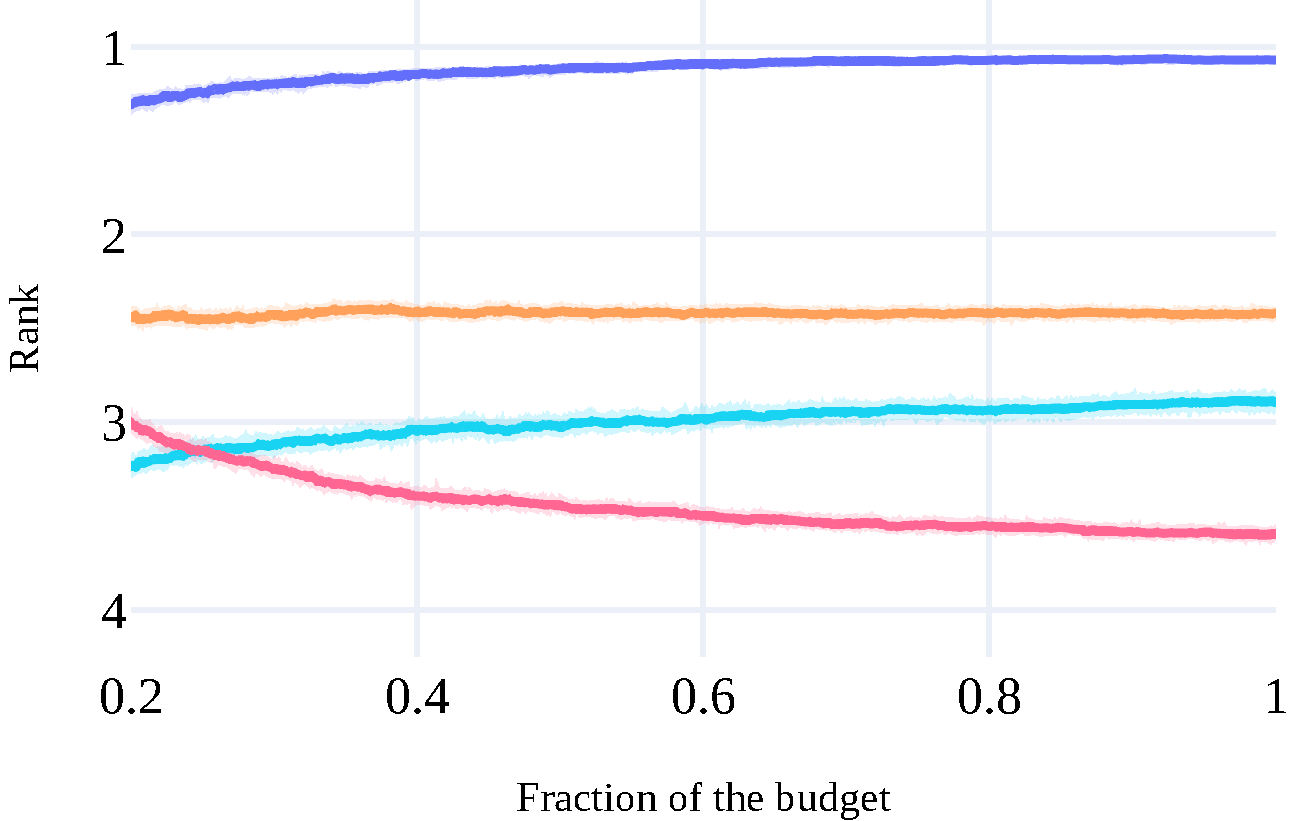
\includegraphics[scale=0.33]{figures/05/figs/figs/ranks/act_all.pdf}
        % \caption{32}
    % \end{subfigure}
    
\includegraphics[scale=0.33]{figures/05/figs/figs/ranks/act_all_legend.pdf}
    \caption{Mean ranks of \texttt{DyMBO} with different acquisition functions as a function of the fraction of the wall-clock time budget on YAHPO Gym and JAHS-Bench-201. Using MACE yields the best performance.}
    \label{fig:ch05:acqs}
\end{figure}

\paragraph{Using different weights for variance.}
\label{sec:ch05:with_variance}
We experimented with weighting the mean and the variance separately by having two, independent weight vectors. 
The weight vector of the mean is the same as described in~\cref{sec:ch05:method}. 
For the variance weights,
% \changed{
we introduce variance error (VE) as a non-probabilistic measure of calibration that does not require additional assumptions about the underlying predictive distribution. In contrast, metrics such as log-likelihood evaluate the full predictive distribution and therefore require a well-specified noise model, which is less straightforward for some surrogates, such as tree-based models.
% }

We define VE for a model $m\in M$ as follows:
% \todo{Could any references for the variance error be included?}
\begin{equation}
    \text{VE}_m(\lambda_t) = \frac{1}{k}\sum_{i=1}^{k} \min \{|(\mu_m(\lambda_t^{(i)}) - \sigma_m(\lambda_t^{(i)}))- c(\lambda_t^{(i)})|,  |(\mu_m(\lambda_t^{(i)}) + \sigma_m(\lambda_t^{(i)}))- c(\lambda_t^{(i)})|\}
\end{equation}
Intuitively, it is the distance to the closest variance bound, as can be seen in~\cref{fig:ch05:gen_res_var}. 
Since computing $\text{VE}_m(\lambda_t)$ relies on the true function value $c(\lambda_t)$, this error can only be calculated post-hoc on points that have already been fully evaluated.
We update the weights for variance accordingly. 
The new weights are defined as:
\begin{equation}\label{eqn:ch05:weight_var}
    {w}'_{t,m}=
    \begin{cases}
        1 & \text{if } \text{VE}_m(\lambda_t)=\text{min}_{l\in M} \text{VE}_l(\lambda_t),  \\
        0 & \text{otherwise},
    \end{cases}
\end{equation}
We calculate the weights for variances using the exponential moving average:
\begin{equation}
    \bar{w}'_{t+1,m} = (1-\alpha) \cdot \bar{w}'_{t, m} + \alpha  \cdot {w}'_{t,m} \; ,
    \label{eq:ch05:weight_ema_var}
\end{equation}
Then, we normalise the weights for the variances independently from the weights for the means:
\begin{equation}
    \hat{w}'_{t,m} = \frac{\bar{w}'_{t,m}}{\sum_{j\in M}{\bar{w}'_{t, j}}},
\end{equation}
Finally, the variance predicted by the ensemble is defined as the weighted sum of the normalised weights of the variances:
\begin{equation}
    \sigma_{\text{ens}}(\lambda)= \sum_{m\in M} \hat{w}'_{t,m} \cdot \sigma_{m}(\lambda).
    \label{eq:ch05:ens_sigma_var}
\end{equation}
% \changed{
We note that VE is a custom metric introduced in this work to measure the accuracy of the predicted uncertainty bounds, analogous to the interval score used in proper scoring rules~\citep{GneRaf07}.
% }

We ran \texttt{DyMBO} with variance with $\alpha=0.9$ and a budget of $100\times$ mean evaluation time per target function. 
Similarly to the results presented in~\cref{sec:ch05:res_general}, we present the mean rank of all methods, including \texttt{DyMBO} with different weights for variances in~\cref{fig:ch05:gen_res_var}. 
The experimental setup is similar to~\cref{sec:ch05:res_general}, where the budget is $100\times$ mean running time of one evaluation. 
We see in~\cref{fig:ch05:diff_var_w} that using different weights for variance ranks worse than \texttt{DyMBO} with the same weights for both the means and variances.
\begin{figure*}
    \centering
    \begin{subfigure}[t]{0.49\textwidth}
        \centering
        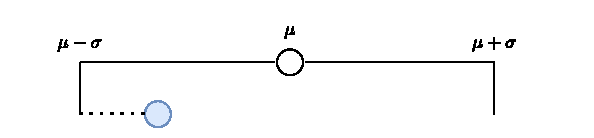
\includegraphics[width=\textwidth]{figures/05/figs/variance/ens_var_error_1.pdf}
        \caption{}
    \end{subfigure}
    \begin{subfigure}[t]{0.49\textwidth}
        \centering
        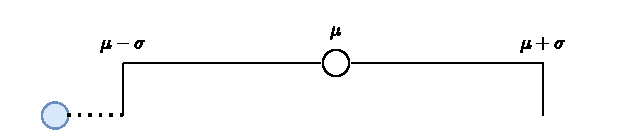
\includegraphics[width=\textwidth]{figures/05/figs/variance/ens_var_error_2.pdf}
        \caption{}
    \end{subfigure}
    \begin{subfigure}[t]{0.49\textwidth}
        \centering
        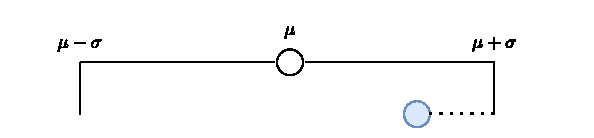
\includegraphics[width=\textwidth]{figures/05/figs/variance/ens_var_error_3.pdf}
        \caption{}
    \end{subfigure}
    \begin{subfigure}[t]{0.49\textwidth}
        \centering
        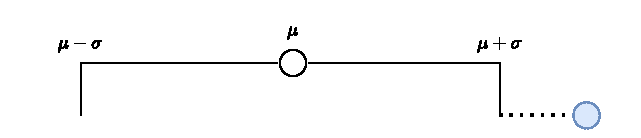
\includegraphics[width=\textwidth]{figures/05/figs/variance/ens_var_error_4.pdf}
        \caption{)}
    \end{subfigure}
    \caption{Illustration of the calculation of the variance error. The white dot is the predicted mean, and the blue dot is the actual value of the target function.
    We distinguish between four cases, depending on whether the actual value of the target function lies within or outside of the uncertainty bounds around the predicted mean, and whether it is smaller or larger than the value of the predicted mean.
    % \todo{Making this a representative example of how the argmin is being used will utilize this plot better.}
    % \aj{I have no idea what this comment means...}
    }
    \label{fig:ch05:gen_res_var}
\end{figure*}

\begin{figure}
    \centering
    % \begin{subfigure}[t]{0.49\textwidth}
    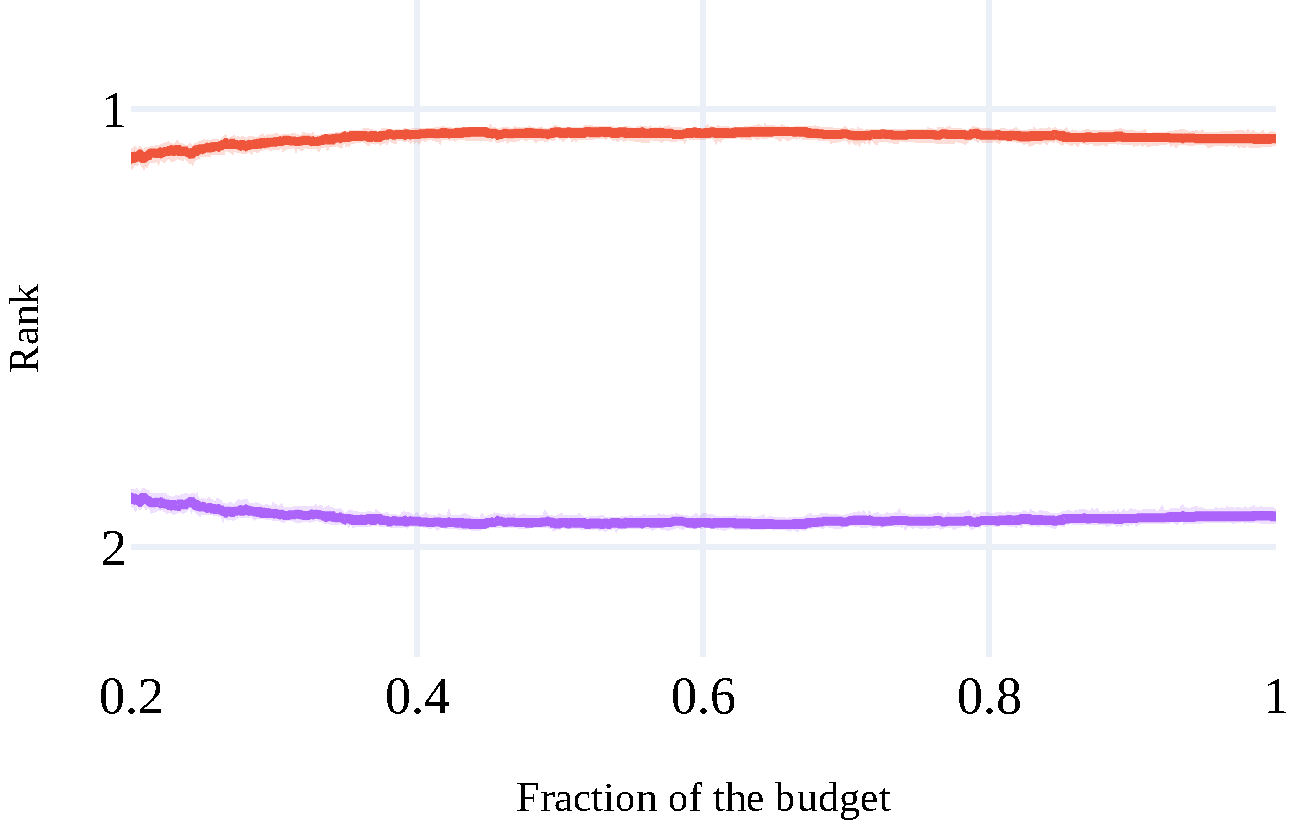
\includegraphics[scale=0.33]{figures/05/figs/figs/ranks/diff_var_w_all.pdf}
    
\includegraphics[scale=0.33]{figures/05/figs/figs/ranks/diff_var_w_all_legend.pdf}
    \caption{Comparison of \texttt{DyMBO} with same weights for means and variances and \texttt{DyMBO} with different weights for means and variances as a function of the fraction of the wall-clock time budget on YAHPO Gym and JAHS-Bench-201. Same weights for means and variances yield better performance.}
    \label{fig:ch05:diff_var_w}
\end{figure}



\paragraph{Using the rule of total variance.}
\label{sec:ch05:abl_totalvar}
We considered computing the variance of the ensemble using the rule of total variance. Such calculation was proposed by~\citet{HutEtAl14} and~\citet{KenGal17}, where the total variance was decomposed into aleatoric uncertainty (noise inherent to the data) and epistemic uncertainty (disagreement between models). We calculate the total variance of the ensemble as follows:
\begin{equation}
    \sigma^2 = \sum_{m\in M} \hat{w}_m \sigma_m^2 + \sum_{m\in M} \hat{w}_m \mu_m^2 - \left(\sum_{m\in M} \hat{w}_m \mu_m\right)^2
\end{equation}

By using the rule of total variance, we add the measure of the correlation between the means and the variances of the models (\emph{i.e.}, epistemic uncertainty) to our initial variance equation that captures aleatoric uncertainty. We ran \texttt{DyMBO} with total variance with $\alpha=0.9$ and a budget of $100\times$ mean evaluation time per target function. We present the results in~\cref{fig:ch05:total_variance}. We see that using total variance ranks worse than \texttt{DyMBO} with aleatoric-only variance.
\begin{figure}
    \centering
    \begin{subfigure}[t]{0.49\textwidth}
    \centering
    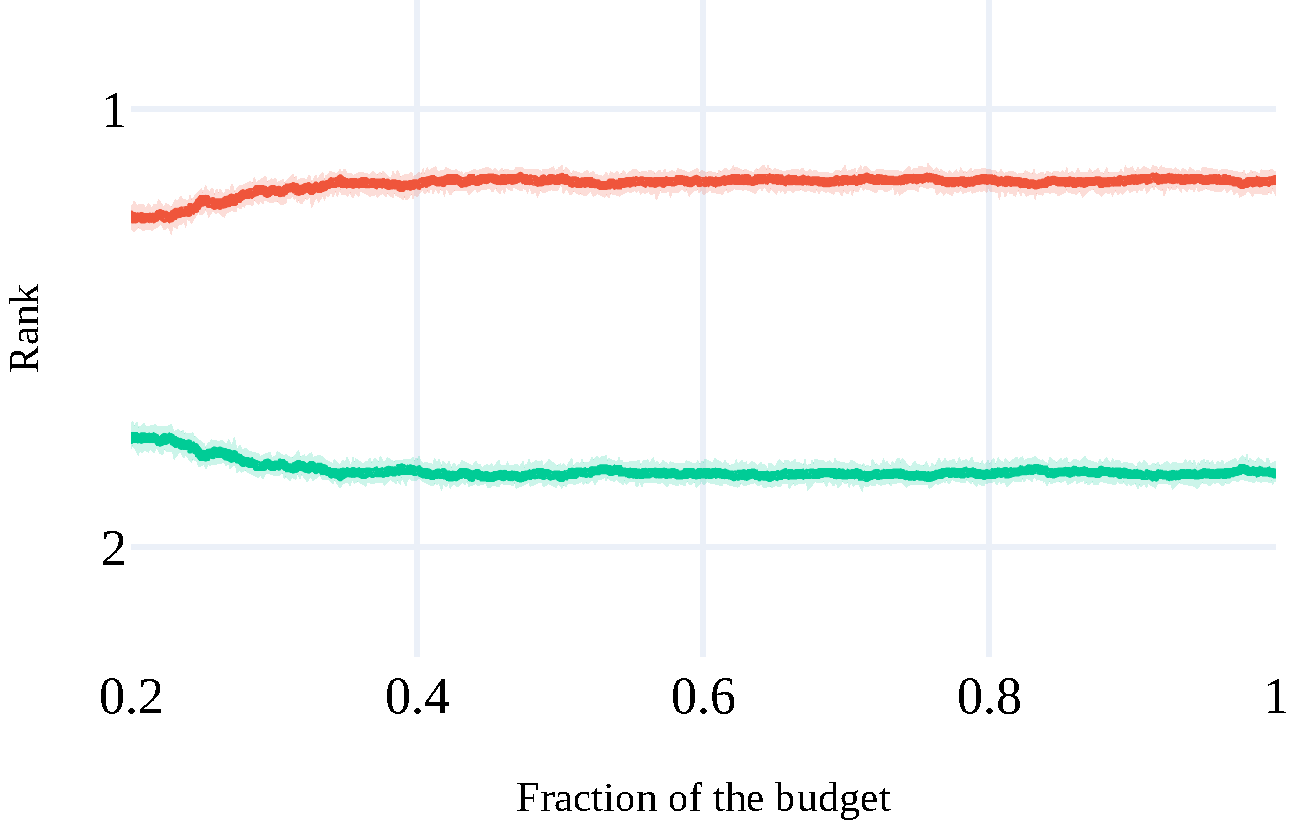
\includegraphics[scale=0.33]{figures/05/figs/figs/ranks/total_variance_all.pdf}
    \end{subfigure}
    \begin{subfigure}[t]{1\textwidth}
        \centering
    
\includegraphics[scale=0.33]{figures/05/figs/figs/ranks/total_variance_all_legend.pdf}
    \end{subfigure}

    \caption{Comparison of \texttt{DyMBO} which computes the variance using the rule of total variance to \texttt{DyMBO} which computes the variance as a weighted sum of the variances as a function of the fraction of the wall-clock time budget on YAHPO Gym and JAHS-Bench-201. Weighted sum of variances yields better performance.}
    \label{fig:ch05:total_variance}
\end{figure}

\paragraph{Considering different loss functions.}
\label{sec:ch05:loss_ablation}
In \texttt{DyMBO}, we use ranking loss as the loss function, as we are interested in identifying where the optimum lies, as opposed to having a model with the most accurate actual predictions. %Indeed, by preserving the pairwise ordering of predicted function values which is to decide which configurations to evaluate next, \emph{i.e.}, to identify promising regions of the search space. 
% The optimisation trajectory relying on the model would therefore still be driven towards promising regions, without using model capacity to perfectly fit the data, which is particularly important when we have limited evaluation budget.
% On the other hand, 
The predictive power of a model is better reflected by more common loss functions for regression tasks, such as mean squared error (MSE). We thus evaluated the performance of \texttt{DyMBO} when using MSE as a metric for model accuracy: 
% \todo{add parameters}\hh{still to be done?}
\begin{equation}
    \text{MSE}(\mu_m, \boldsymbol{\lambda}) = \frac{1}{n} \cdot\sum_{\lambda^{(j)}\in \boldsymbol{\lambda}} (\mu_m(\lambda^{(j)}) - c(\lambda^{(j)}))^2.
\end{equation}
We ran \texttt{DyMBO} with MSE as a loss function on YAHPO Gym and JAHS-Bench-201 with a budget of $100\times$ mean evaluation time per target function. We present the results in~\cref{fig:ch05:loss_ablation}. We see that \texttt{DyMBO} using ranking loss performs slightly better than \texttt{DyMBO} using MSE.
\begin{figure}
    \centering
    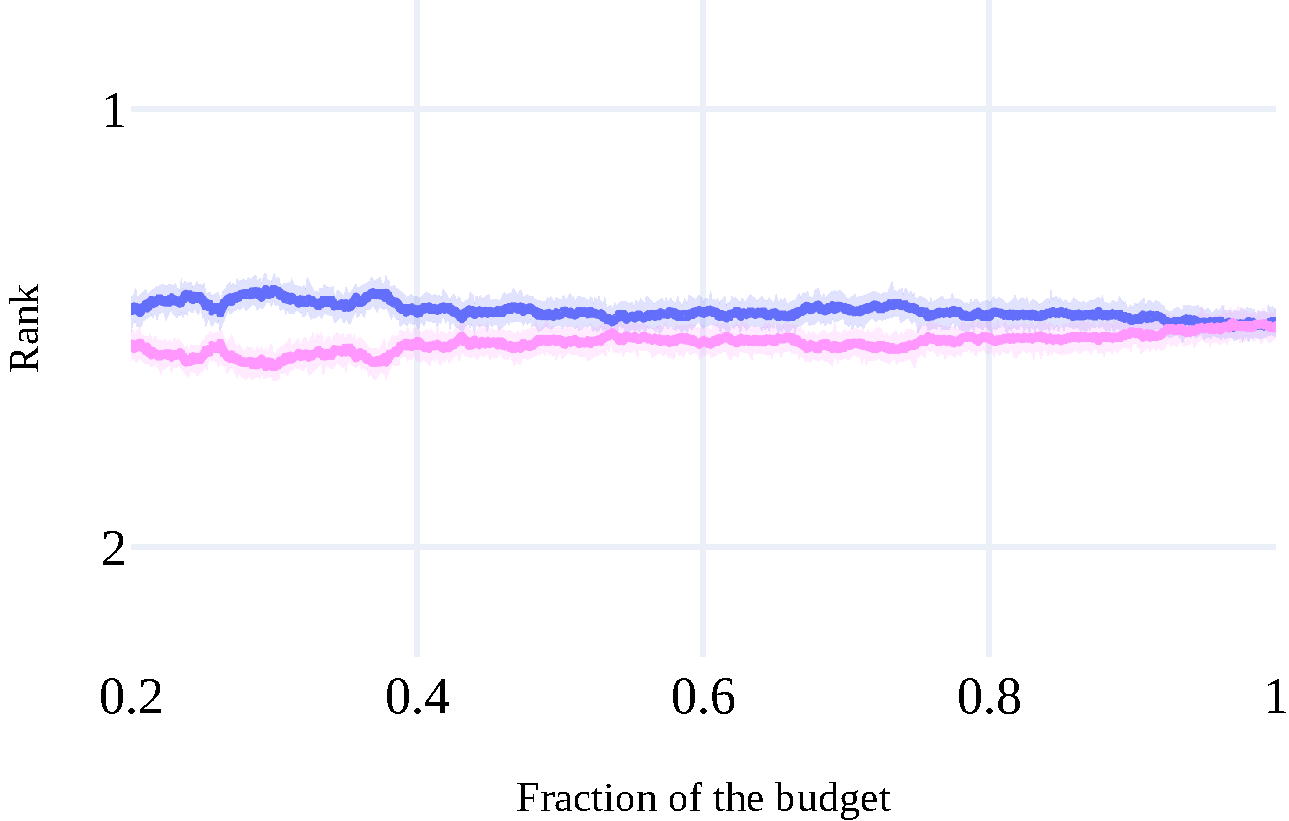
\includegraphics[scale=0.33]{figures/05/figs/figs/ranks/loss_all.pdf}
    
\includegraphics[scale=0.33]{figures/05/figs/figs/ranks/loss_all_legend.pdf}

    \caption{Mean ranks of \texttt{DyMBO} with different loss functions (ranking loss vs. MSE) as a function of the fraction of the wall-clock time budget on YAHPO Gym and JAHS-Bench-201. Ranking loss performs better than MSE, especially in low budgets.}
    \label{fig:ch05:loss_ablation}
\end{figure}

\paragraph{Varying the combinations of surrogate models in the ensemble.}
\label{sec:ch05:models_choice}
We evaluated the performance of \texttt{DyMBO} with different surrogate models as part of the ensemble. Having more surrogate models allows for better best-found configurations 
% \aj{what do we mean by maximal results?}\er{best-found results?}\aj{I would replace it with "best-found solutions" or "configurations", pls check how it reads} 
as the ensemble can choose the best model for each target function. However, including more models also increases the risk of choosing a model that performs poorly. We ran \texttt{DyMBO} with different combinations of 4 surrogate models: RF, GP, GB, and ET. We used a budget of $100\times$ mean evaluation time per target function. We present the results in~\cref{fig:ch05:models_choice}. We observe best performance by using only RF and GP, followed by using RF, GP and ET.
\begin{figure}
    \centering
    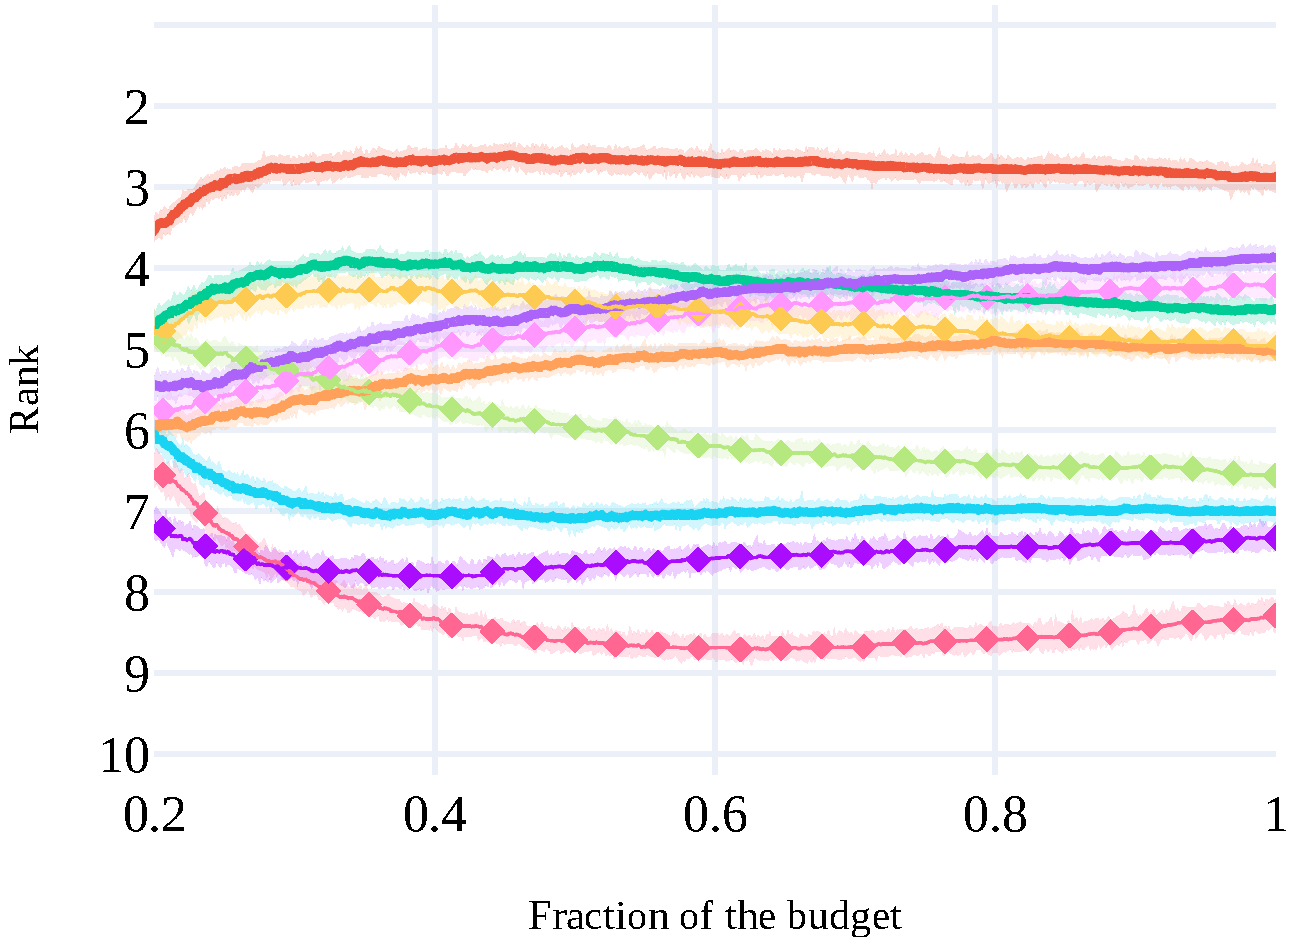
\includegraphics[scale=0.33]{figures/05/figs/figs/ranks/models_choice_all.pdf}
    
\includegraphics[scale=0.33]{figures/05/figs/figs/ranks/models_choice_all_legend.pdf}
    \caption{Mean ranks of \texttt{DyMBO} with different surrogate models as a function of the fraction of the wall-clock time budget on YAHPO Gym and JAHS-Bench-201. Using the combination of RF and GP yields the best performance.}
    \label{fig:ch05:models_choice}
\end{figure}

\paragraph{Using different weight initialisation strategies.}
\label{sec:ch05:init_ablation}
We experimented with different weight initialisation schemes to assess how they affect the performance of \texttt{DyMBO}. In addition to initialising with RF (with $w_{RF}=1$ and $w_{GP}=0$ as in~\cref{sec:ch05:experiments}), we also considered initialising with GP: $w_{GP}=1$ and $w_{RF}=0$. Additionally, we tested initialising with both models: $w_{RF}=1$ and $w_{GP}=1$. Finally, we tried a heuristic initialisation, where we set $w_{RF}=1$ if the target function has categorical hyperparameters, and $w_{GP}=1$ if the target function is cheap. The rest of the weights are set to 0. 
% \er{Just a comment about aesthetics... many times in the manuscript, the last line of a paragraph is composed of 1 word only. Am I allowed to slightly shorten so that this does not happen? Maybe we can also gain some space given the page limit.} \aj{I agree and also don't like a short last sentence. If you have an idea on how to shorten so that the meaning stays the same, please go ahead :)}

We ran \texttt{DyMBO} with different weight initialisation schemes on YAHPO Gym and JAHS-Bench-201 with a budget of $100\times$ mean evaluation time per target function. We show the results in~\cref{fig:ch05:init-ablation}. We see similar ranks between the different initialisation schemes, with the best performance achieved by initialising with RF.

\begin{figure}
    \centering
    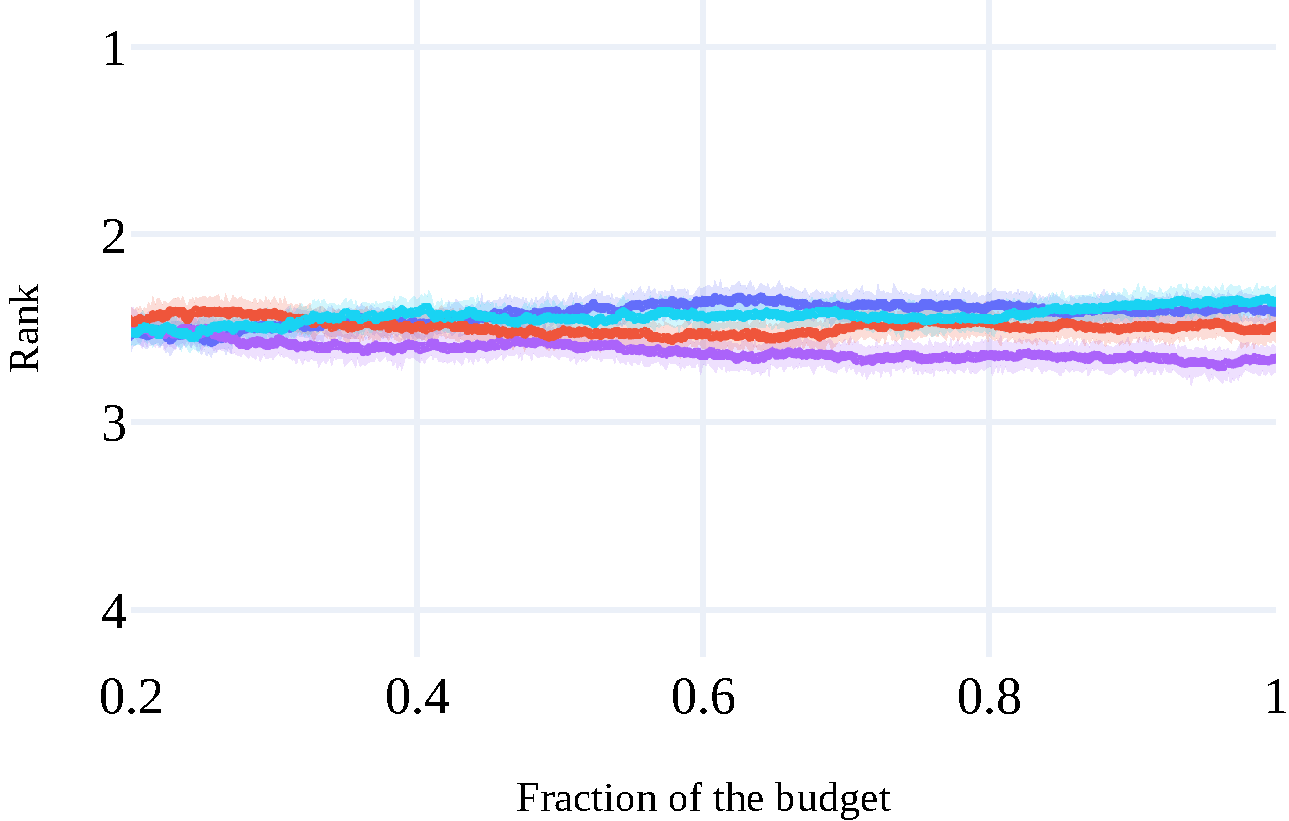
\includegraphics[scale=0.33]{figures/05/figs/figs/ranks/init_ablation_all.pdf}
    
\includegraphics[scale=0.33]{figures/05/figs/figs/ranks/init_ablation_all_legend.pdf}
    \caption{Mean ranks of \texttt{DyMBO} with different initialisation schemes as a function of the fraction of the wall-clock time budget on YAHPO Gym and JAHS-Bench-201.  Initialising with RF yields the best performance, although the differences are small.}
    \label{fig:ch05:init-ablation}
\end{figure}

\paragraph{Varying the number of points for accuracy evaluation.}
\label{sec:ch05:abl_eval_all}

We tested whether evaluating the model accuracy on all previously sampled points (\emph{i.e.}, the full history of observations) yields better performance than evaluating only on the last batch of points (\emph{i.e.}, observations from the last iteration only, which corresponds to having a train-test split). In the latter setting, computation of the new weights for the models was adapted accordingly so as to depend only on the accuracy from the last iteration. We ran \texttt{DyMBO} in this setting with a budget of $100\times$ mean evaluation time per target function. We show the results in~\cref{fig:ch05:eval-all}. We see that evaluating on the entire history of observations yields better performance than evaluating only on the last batch of points.
\begin{figure}
    \centering
    \centering
    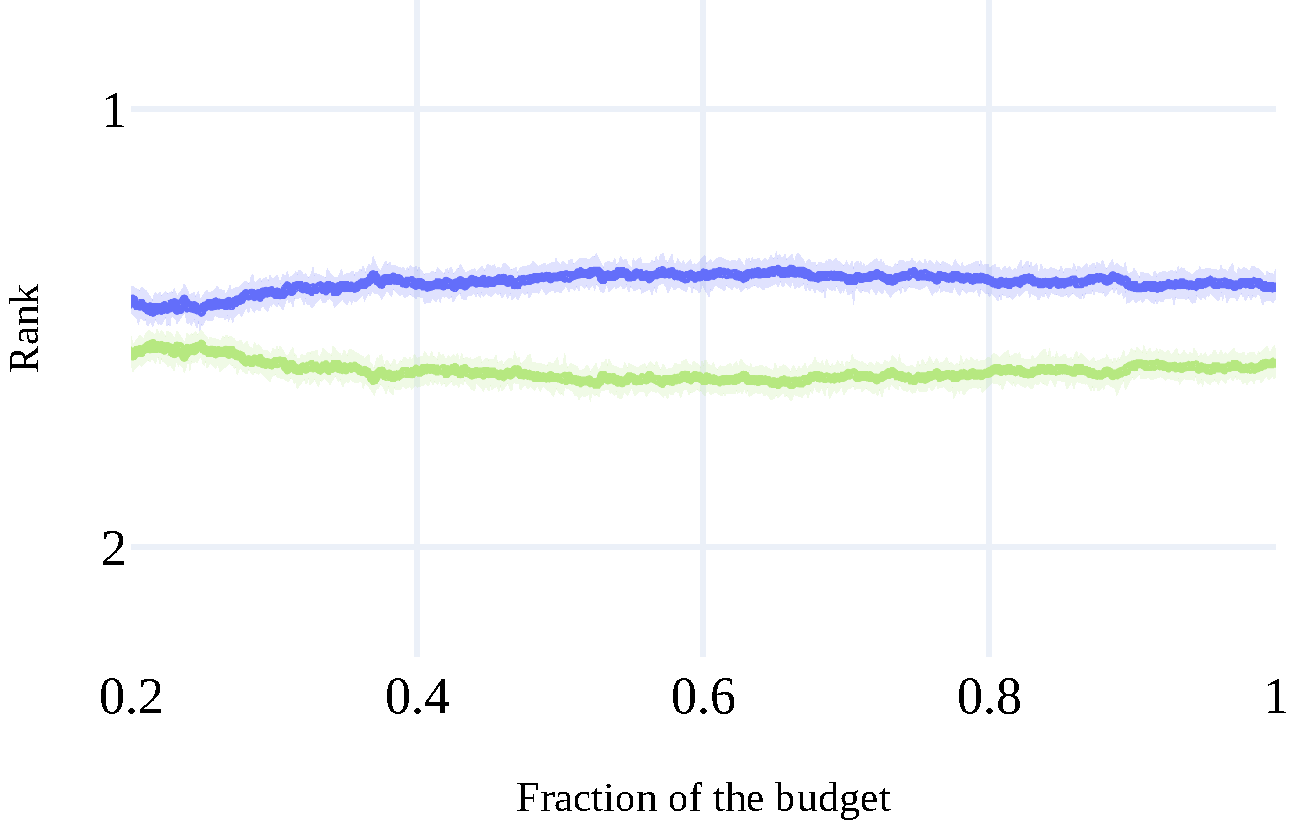
\includegraphics[scale=0.33]{figures/05/figs/figs/ranks/eval_all_all.pdf}
    
\includegraphics[scale=0.33]{figures/05/figs/figs/ranks/eval_all_all_legend.pdf}
    \caption{Comparison of original \texttt{DyMBO} (which evaluates on all points) to \texttt{DyMBO} which evaluates only on the last batch of points as a function of the fraction of the wall-clock time budget on YAHPO Gym and JAHS-Bench-201.
    % \todo{legend}
    }
    \label{fig:ch05:eval-all}
\end{figure}

\section{Results per search space}
\label{sec:ch05:res-search-space}

We analysed the performance of our method based on search space characteristics, offering insights into the efficacy of dynamic ensembling and selection of different surrogates that excel in various types of search spaces.
We provide the results for mixed discrete-continuous and numerical search spaces in~\cref{fig:ch05:search-spaces1,fig:ch05:search-spaces2}.
We see that all \texttt{DyMBO} variants are consistently top-ranked regardless of the nature of the search space, with exception of the rbv2\_svm scenario in~\cref{fig:ch05:rbv2_svm}, based on optimising hyperparameters of a support vector machine (SVM), for which Optuna AutoSampler exhibits the best performance.
% \todo{check if true, legend}

For certain mixed discrete-continuous search spaces, \emph{e.g.,} scenarios in~\cref{fig:ch05:rbv2_aknn,fig:ch05:rbv2_ranger,fig:ch05:rbv2_rpart}, \texttt{DyMBO} variants with $\alpha = 0.9$ and $\alpha = 1.0$ perform notably well, with low variance in performance, emphasising the advantage of either a strong reliance on the newly assigned weights or a pure selection in those cases.
For other mixed discrete-continuous spaces, \emph{e.g.,} scenarios in~\cref{fig:ch05:rbv2_glmnet,fig:ch05:rbv2_super,fig:ch05:rbv2_xgboost}, \texttt{DyMBO} variants with medium or very low values of $\alpha$ are top performers, revealing that our method can leverage not only the complementary strengths of different surrogates, but that having a possibility to rely more strongly on the history of surrogate accuracies can be crucial for the overall performance of the method.
For numerical-only search space in~\cref{fig:ch05:lcbench}, all \texttt{DyMBO} variants outperform single surrogates and other HPO methods, with a notable gap in ranks between \texttt{DyMBO} and the next-best method.

\begin{figure*}
    \centering
    \begin{subfigure}[t]{0.49\textwidth}
        \centering
        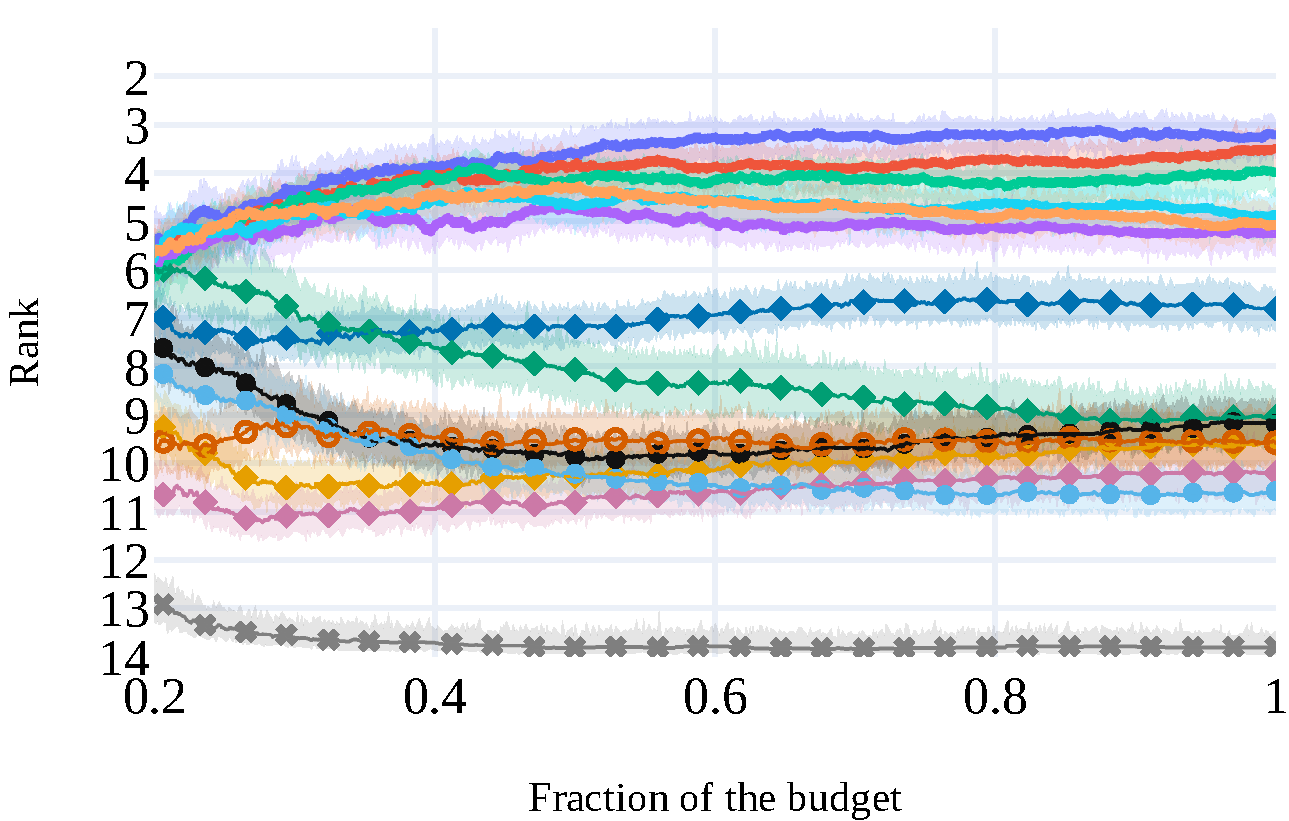
\includegraphics[scale=0.33]{figures/05/figs/figs/ranks/main_ranks_rbv2_aknn.pdf}
        \caption{rbv2\_aknn: $6D$ mixed discrete-continuous search space}
        \label{fig:ch05:rbv2_aknn}
    \end{subfigure}
    \begin{subfigure}[t]{0.49\textwidth}
        \centering
        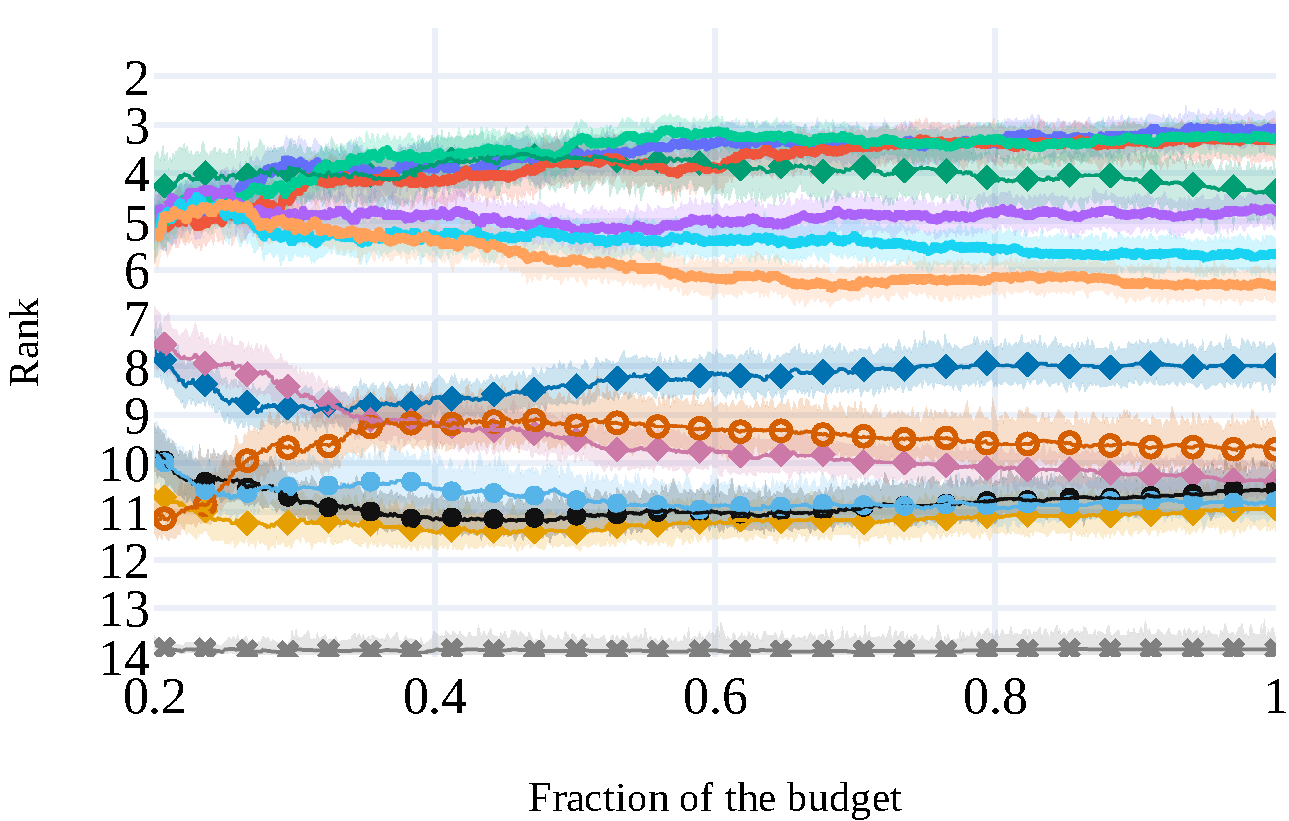
\includegraphics[scale=0.33]{figures/05/figs/figs/ranks/main_ranks_rbv2_glmnet.pdf}
        \caption{rbv2\_glmnet: $3D$ mixed discrete-continuous search space}
        \label{fig:ch05:rbv2_glmnet}
    \end{subfigure}
        \begin{subfigure}[t]{0.49\textwidth}
        \centering
        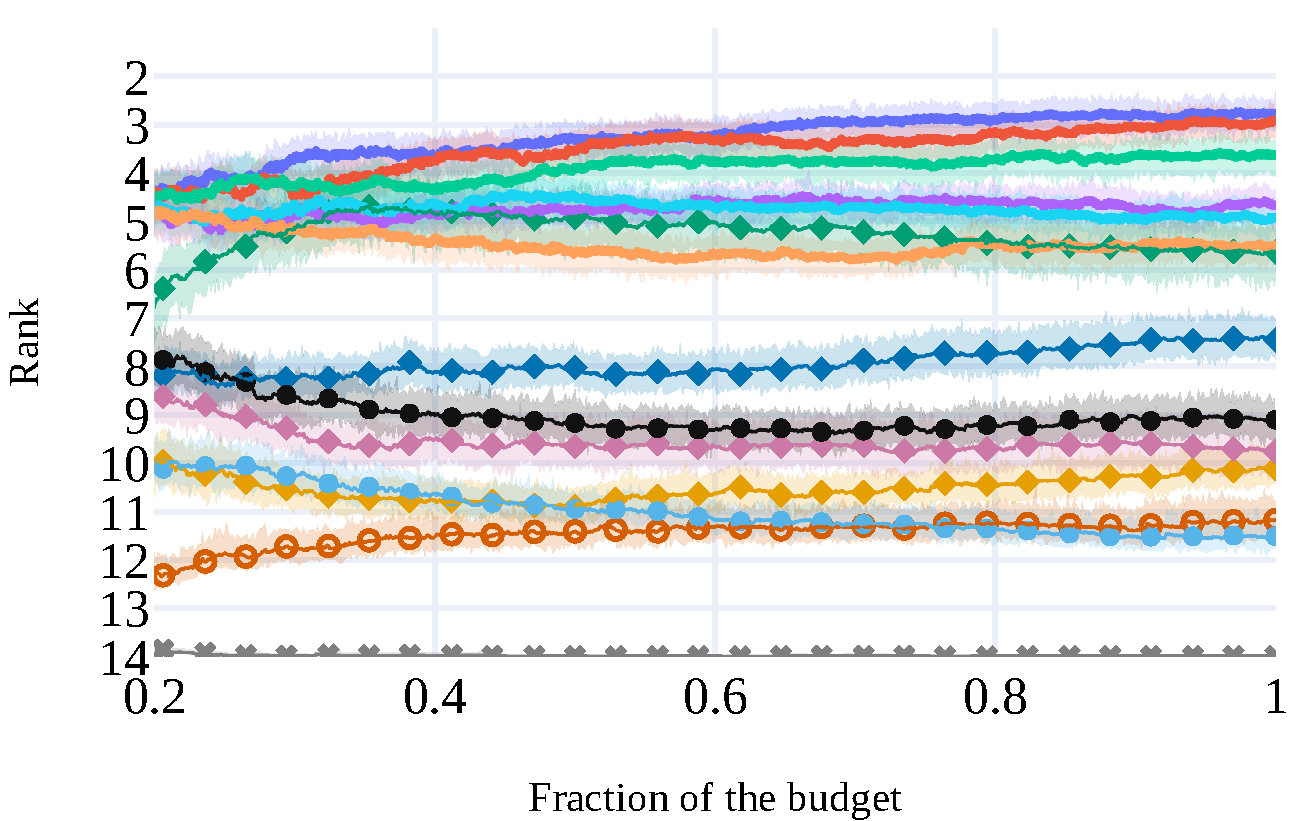
\includegraphics[scale=0.33]{figures/05/figs/figs/ranks/main_ranks_rbv2_ranger.pdf}
        \caption{rbv2\_ranger: $8D$ mixed discrete-continuous search space}
        \label{fig:ch05:rbv2_ranger}
    \end{subfigure}
        \begin{subfigure}[t]{0.49\textwidth}
        \centering
        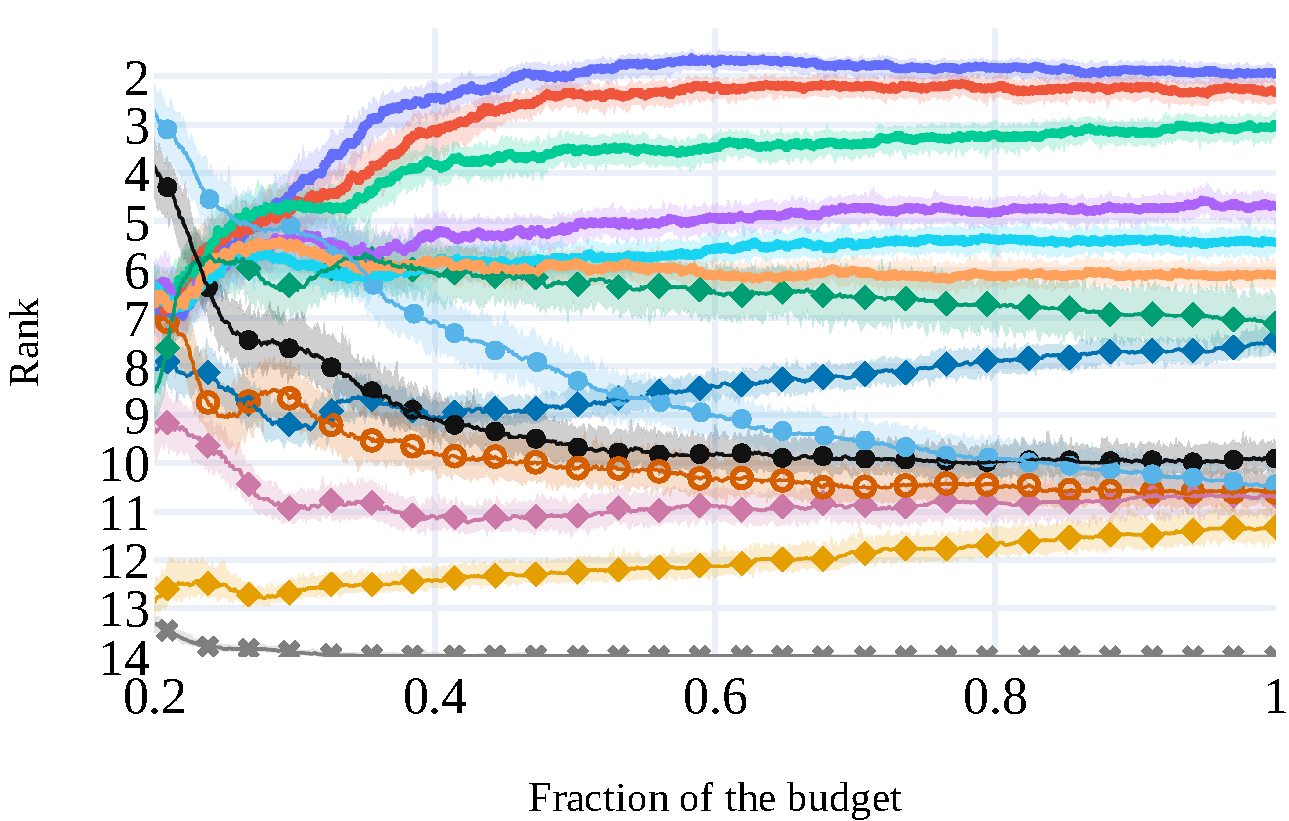
\includegraphics[scale=0.33]{figures/05/figs/figs/ranks/main_ranks_rbv2_rpart.pdf}
        \caption{rbv2\_rpart: $5D$ mixed discrete-continuous search space}
        \label{fig:ch05:rbv2_rpart}
    \end{subfigure}
    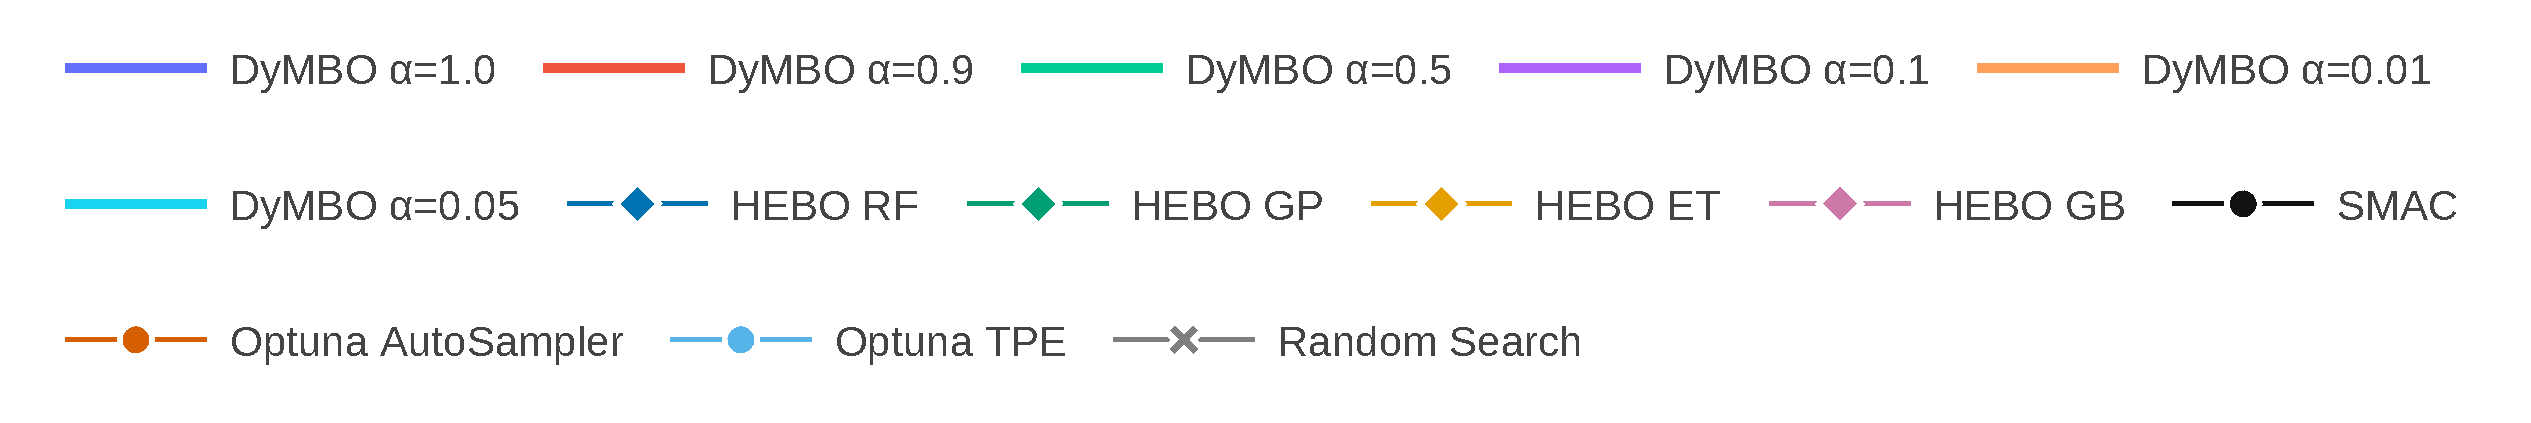
\includegraphics[scale=0.33]{figures/05/figs/figs/ranks/main_ranks_rbv2_xgboost_legend.pdf}
    \caption{Mean ranks of \texttt{DyMBO} (with different values of $\alpha$), HEBO with different surrogate models, and other HPO methods, as a function of the fraction of the wall-clock time budget on benchmarks from YAHPO Gym, split by search space characteristics (mixed discrete-continuous or numerical only). Variants of \texttt{DyMBO} are consistently top-ranked across different types of search spaces and different dimensionalities.
    }
    \label{fig:ch05:search-spaces1}
\end{figure*}

\begin{figure*}
    \centering
    \begin{subfigure}[t]{0.49\textwidth}
        \centering
        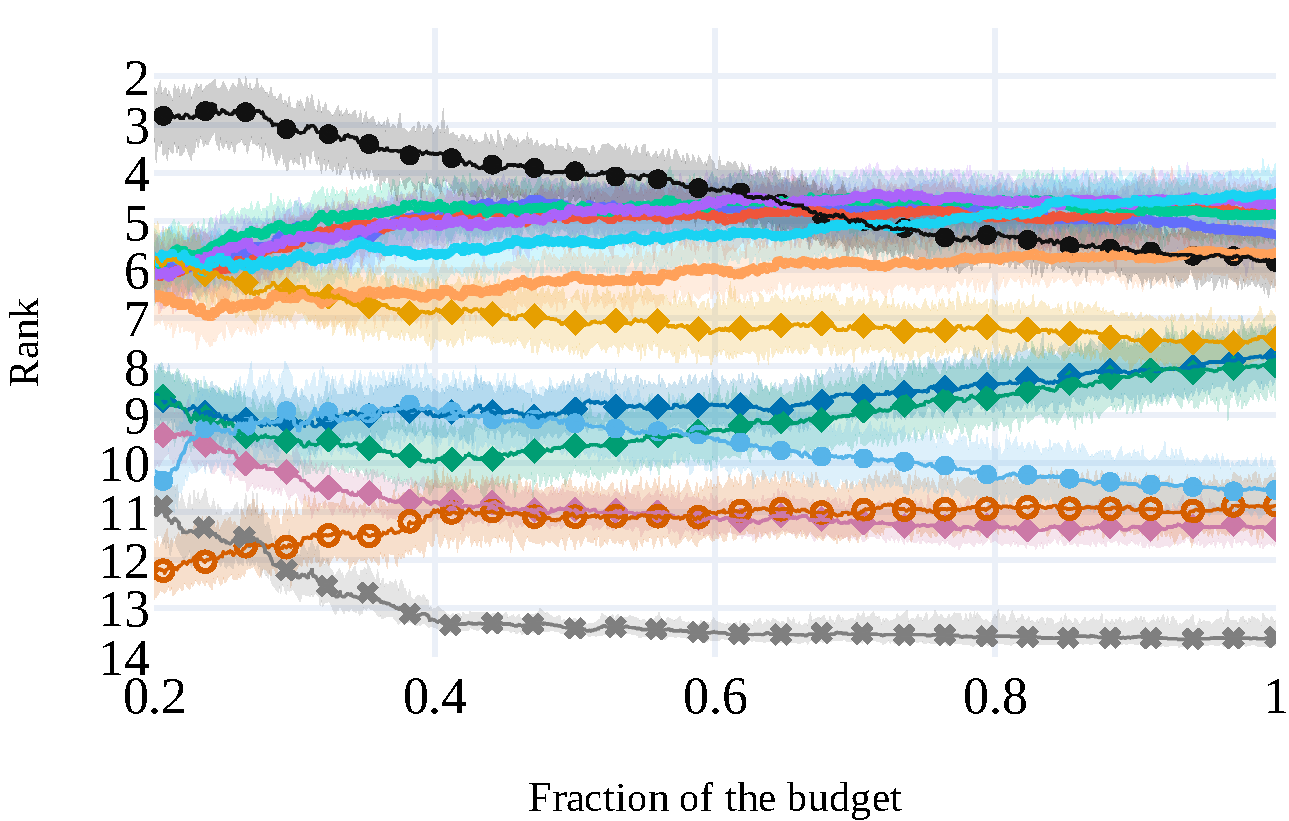
\includegraphics[scale=0.33]{figures/05/figs/figs/ranks/main_ranks_rbv2_super.pdf}
        \caption{rbv2\_super: $38D$ mixed discrete-continuous search space}
        \label{fig:ch05:rbv2_super}
    \end{subfigure}
    \begin{subfigure}[t]{0.49\textwidth}
        \centering
        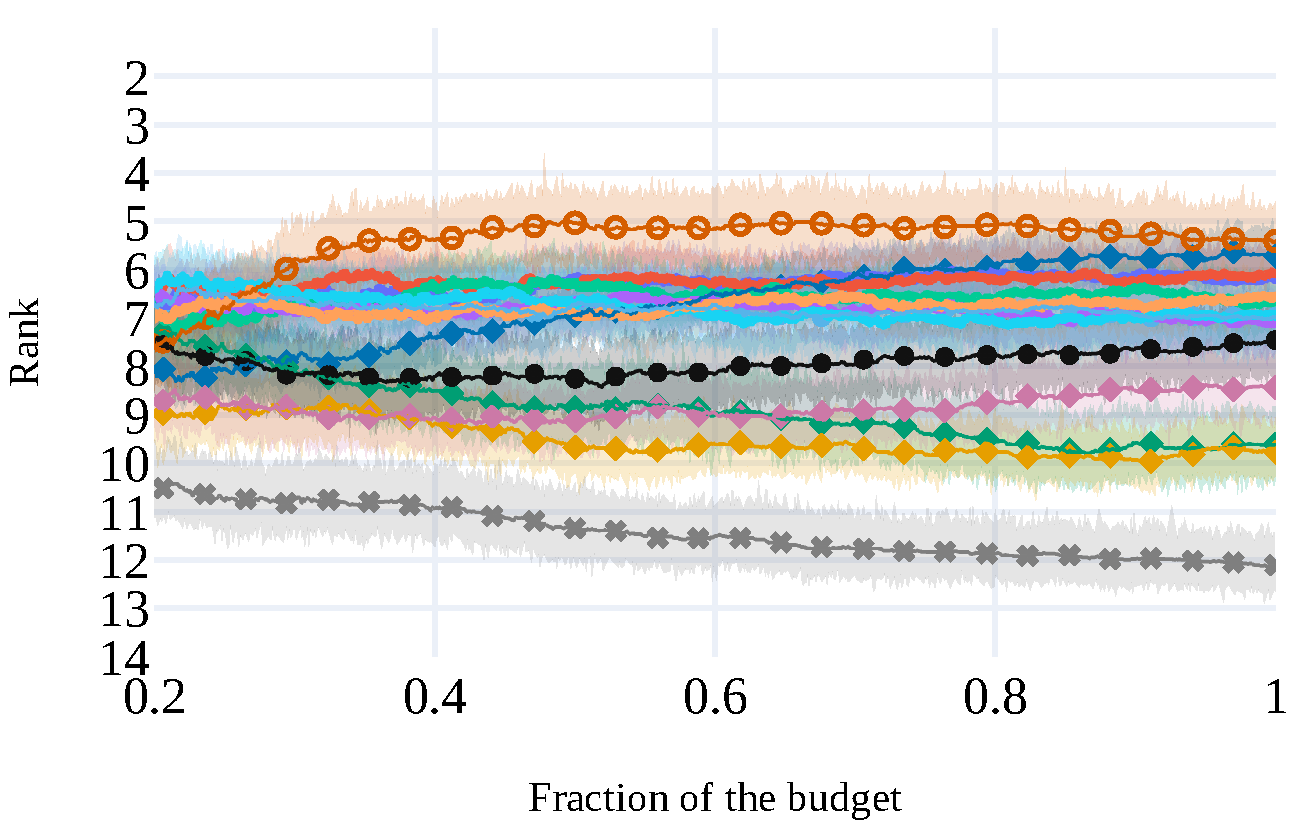
\includegraphics[scale=0.33]{figures/05/figs/figs/ranks/main_ranks_rbv2_svm.pdf}
        \caption{rbv2\_svm: $6D$ mixed discrete-continuous search space}
        \label{fig:ch05:rbv2_svm}
    \end{subfigure}
    \begin{subfigure}[t]{0.49\textwidth}
        \centering
        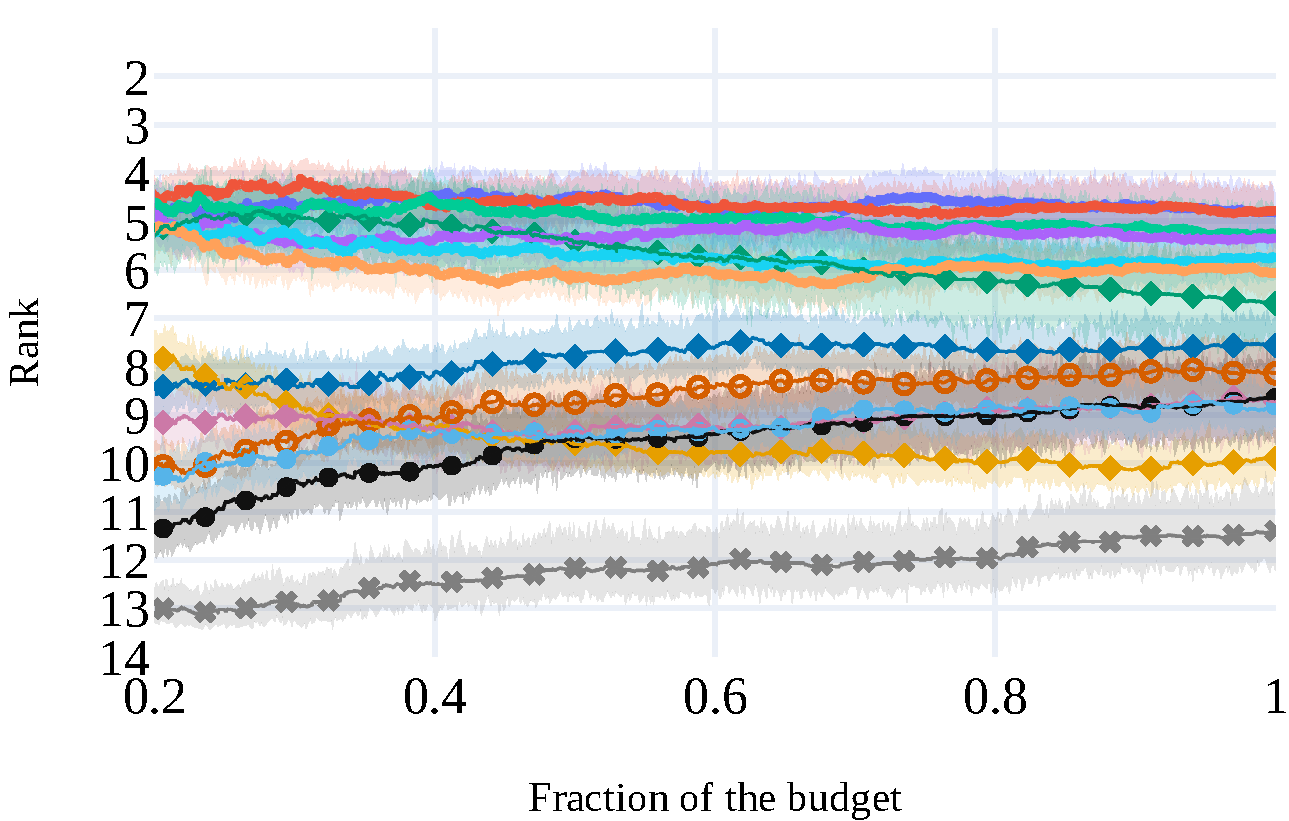
\includegraphics[scale=0.33]{figures/05/figs/figs/ranks/main_ranks_rbv2_xgboost.pdf}
        \caption{rbv2\_xgboost: $14D$ mixed discrete-continuous search space}
        \label{fig:ch05:rbv2_xgboost}
    \end{subfigure}
    \begin{subfigure}[t]{0.49\textwidth}
        \centering
        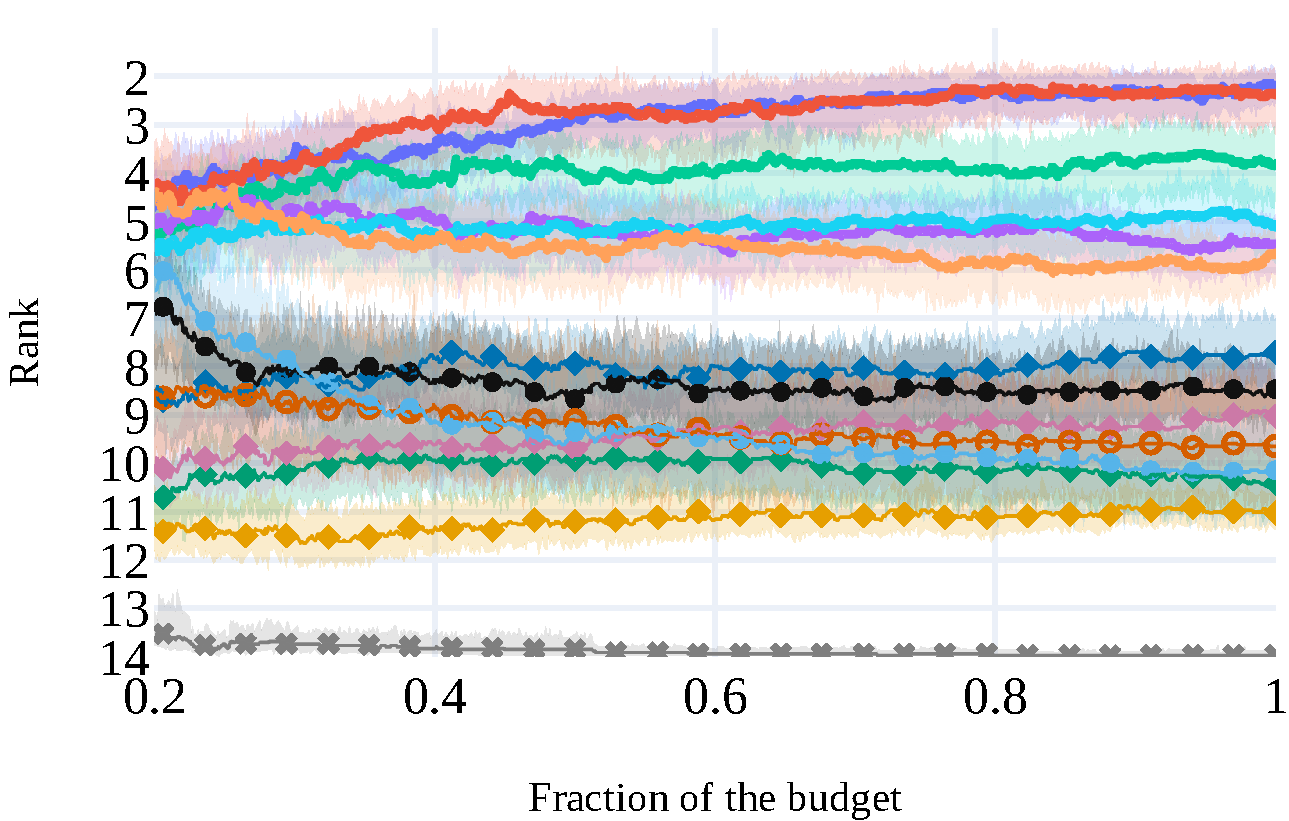
\includegraphics[scale=0.33]{figures/05/figs/figs/ranks/main_ranks_lcbench.pdf}
        \caption{lcbench: $7D$ numerical search space}
        \label{fig:ch05:lcbench}
    \end{subfigure}
    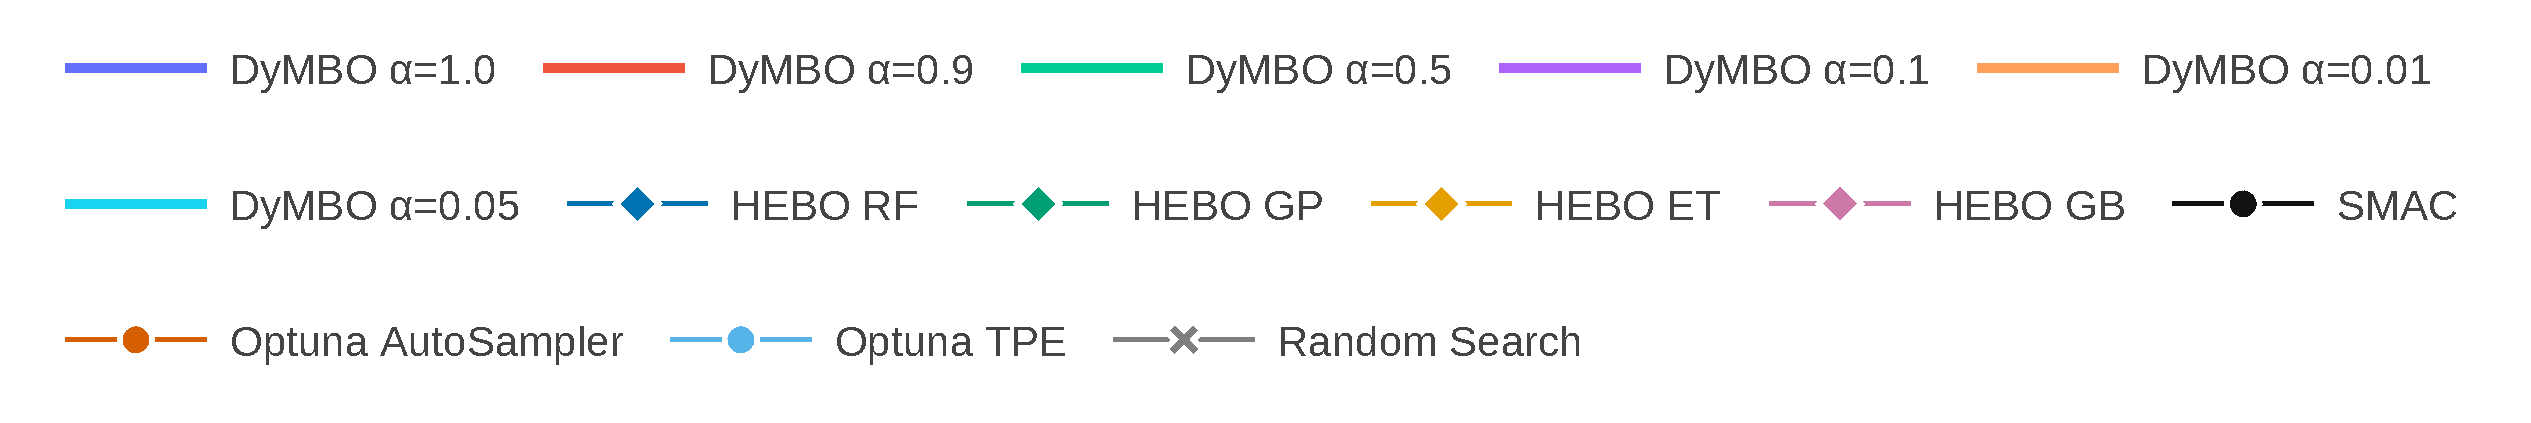
\includegraphics[scale=0.33]{figures/05/figs/figs/ranks/main_ranks_rbv2_xgboost_legend.pdf}
    \caption{Mean ranks of \texttt{DyMBO} (with different values of $\alpha$), HEBO with different surrogate models, and other HPO methods, as a function of the fraction of the wall-clock time budget on benchmarks from YAHPO Gym, split by search space characteristics (mixed discrete-continuous or numerical only). Variants of \texttt{DyMBO} are consistently top-ranked across different types of search spaces and different dimensionalities.
    }
    \label{fig:ch05:search-spaces2}
\end{figure*}

\section{Benchmark details}
\label{sec:ch05:benchs}

\textbf{Yet Another HPO Benchmark (YAHPO) Gym}~\citep{PfiEtAl22} is a surrogate-based benchmark for hyperparameter optimisation on tabular machine learning tasks. 
The benchmark consists of multiple datasets from OpenML and various machine learning algorithms. 
The authors provide a surrogate model for each machine learning algorithm and a dataset that predicts different objectives, such as accuracy, training time, and more.

YAHPO Gym contains several scenarios. 
Each scenario has a configuration space and is based on a machine learning algorithm. 
Each scenario contains multiple datasets, which are called instances. 
The YAHPO Gym scenarios are: \\
% \begin{itemize}
    \textbf{rbv2\_ranger}~\citep{BinEtAl20}: RF using the ranger R implementation.\\ 
    \textbf{rbv2\_rpart}~\citep{BinEtAl20}: decision tree using the mlr implementation.\\
    \textbf{rbv2\_glmnet}~\citep{BinEtAl20}: generalised linear models (GLM) with elastic net regularisation using the mlr implementation.\\
    \textbf{rbv2\_svm}~\citep{BinEtAl20}: support vector machine (SVM) with the mlr implementation.\\
    \textbf{rbv2\_xgboost}~\citep{BinEtAl20}: gradient boosting using XGBoost.\\
    \textbf{rbv2\_aknn}~\citep{BinEtAl20}: k-nearest neighbours using the mlr implementation.\\
    \textbf{rbv2\_super}~\citep{BinEtAl20}: a combined algorithm selection and hyperparameter optimisation (CASH) scenario that uses all the above rbv2 scenarios.\\
    \textbf{iaml\_glment}~\citep{PfiEtAl22}: generalised linear models (GLM) with elastic net regularisation using the mlr implementation.\\
    \textbf{iaml\_rpart}~\citep{PfiEtAl22}: decision tree using the mlr implementation.\\
    \textbf{iaml\_ranger}~\citep{PfiEtAl22}: RF using the ranger R implementation.\\
    \textbf{iaml\_xgboost}~\citep{PfiEtAl22}: gradient boosting using XGBoost.\\
    \textbf{iaml\_super}~\citep{PfiEtAl22}: combined algorithm selection and hyperparameter optimisation (CASH) scenario that uses all the above iaml scenarios.\\
    \textbf{LCBench}~\citep{ZimEtAl21}: optimising the training hyperparameters and architecture of multi-layer perceptron on tabular datasets.\\
    \textbf{FCNet}~\citep{FalEtAl18}: hyperparameter optimisation of a fully-connected network for tabular data.\\
    \textbf{NAS-Bench-301}~\citep{ZelEtAl22}: neural architecture search (NAS) scenario using a constant set of training hyperparameters. The search space describes a cell of the neural network and the hyperparameters are different operations done in each cell.
% \end{itemize}

For details on configuration spaces, we refer the reader to original papers.
The configuration spaces for the rbv2 scenarios are taken from~\citep{BinEtAl20}. 
For rbv2\_super, the configuration space contains all the configuration spaces of individual algorithms, with an additional hyperparameter which selects the algorithm. 
The configuration spaces for the iaml scenarios are taken from~\citep{PfiEtAl22}; the iaml\_super scenario is similar to rbv2\_super, where there is an additional hyperparameter to select the algorithm. 
While the iaml and rbv2 scenarios look similar, there are a few differences in the configuration space. 
First, the configuration space of rbv2 contains the input imputation used, while in iaml the input imputation is constant. 
Another difference is a different range of hyperparameters (for example, the number of rounds in XGBoost). 
In all scenarios, the target metric is accuracy, as defined in~\citep{PfiEtAl22}.  
The configuration spaces for LCBench, FCNet and NAS-Bench-301 are taken from~\citep{ZimEtAl21,FalEtAl18,ZelEtAl22}, respectively.
Additionally, we benchmarked our method on \textbf{JAHS-Bench-201}~\citep{BanEtAl22}: a neural architecture search (NAS) benchmark that optimises both the architecture of the neural network and the training hyperparameters. The benchmark contains three datasets: CIFAR10, Fashion MNIST and Colorectal Histology.

\paragraph{Evaluation budget.}
All YAHPO Gym and JAHS-Bench-201 surrogates predict the running time required to train and evaluate the model using a specific configuration. 
Therefore, we calculate the budget per instance similarly to~\citet{EggEtAl21}: we sample 1\,000 uniform random configurations per instance and predict the required running time.
We then calculate the mean running time per instance. 
The budget for each optimisation is then $100\times $ mean running time of the instance. 
% The running times per scenario are available in~\autoref{fig:running-times}.
% ~\autoref{fig:cdf_budgets}. \aj{what figure are we referencing?}


% \begin{figure}
%     \centering
%     \includegraphics{figs/budget_info.pdf}
%     \caption{Cumulative number of instances as a function of the budget for every instance, for each scenario. \emph{E.g.}, 60 instances from the iaml\_glmnet scenario (in medium green with a dot) take up to 100 seconds to evaluate. \aj{can be removed to save space}\er{I would be in favor of removing it.}}
%     \label{fig:cdf_budgets}
% \end{figure}

\section{Additional benchmarks}
\label{sec:ch05:add-bench}

We have shown that \texttt{DyMBO} outperforms all baselines on YAHPO Gym and JAHS-Bench-201 across a wide range of settings, emphasising its strong performance on mixed discrete-continuous domains.
In this section, we report results of our method on two additional benchmarks: on synthetic continuous functions in order to illustrate good performance of \texttt{DyMBO} on purely numerical search spaces, and on HPOBench, in order to confirm good performance of \texttt{DyMBO} on a classic, widely studied HPO benchmark suite.

\subsection{Synthetic continuous functions}
\label{sec:ch05:synth-cont-func}

We empirically evaluated our method on purely numerical search spaces by considering six synthetic continuous target functions, widely used in studies on design and development of novel black-box optimisation methods and benchmarks.
Specifically, we used the $10$-dimensional Ackley, Hachevsky, Griewank, Himmelblau, Schaffer and Schwefel functions, in their native HEBO implementation.
The experimental setup used here is the same as the default described in~\cref{sec:ch05:experiments}.

We show in~\cref{fig:ch05:synth-cont} the convergence behaviour of \texttt{DyMBO} and the single-surrogate HEBO baselines on those functions.
\texttt{DyMBO} achieves faster or competitive convergence and reaches a lower or comparable final regret across most benchmarks.
The advantage of \texttt{DyMBO} is most pronounced on the multimodal functions: on Ackley and Schwefel, \texttt{DyMBO} converges faster than all single-surrogate baselines and achieves a lower final regret, suggesting that our method is better equipped to navigate complex, multimodal landscapes.

On Griewank and Hachevsky, \texttt{DyMBO} again outperforms all baselines in terms of final regret, with standalone GP being the closest competitor.
On Schaffer, the differences between methods are smaller, and \texttt{DyMBO} remains competitive without a clear advantage, while on Himmelblau, all methods converge rapidly to near-zero regret within the first few iterations.
This suggests that these functions are not informative enough to distinguish between the methods.
Among the single-surrogate baselines, GP tends to perform competitively on smoother functions, while tree-based surrogates show weaker performance on more complex landscapes, further motivating the dynamic surrogate tailoring approach of \texttt{DyMBO}.

\begin{figure*}
    \centering
    \begin{subfigure}[t]{0.49\textwidth}
        \centering
        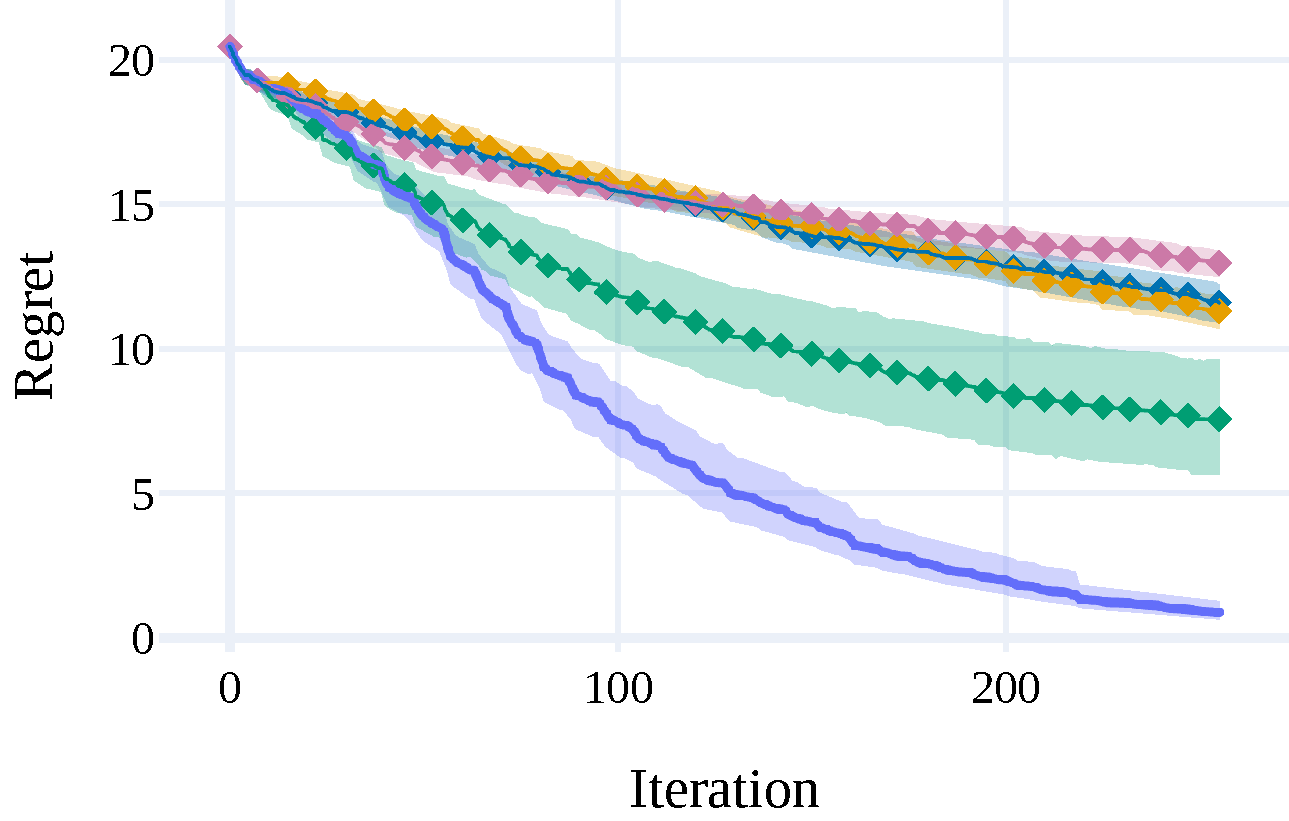
\includegraphics[scale=0.33]{figures/05/figs/figs/continuous/co_8_init_fackley_time.pdf}
        \caption{Ackley}
    \end{subfigure}
    \begin{subfigure}[t]{0.49\textwidth}
        \centering
        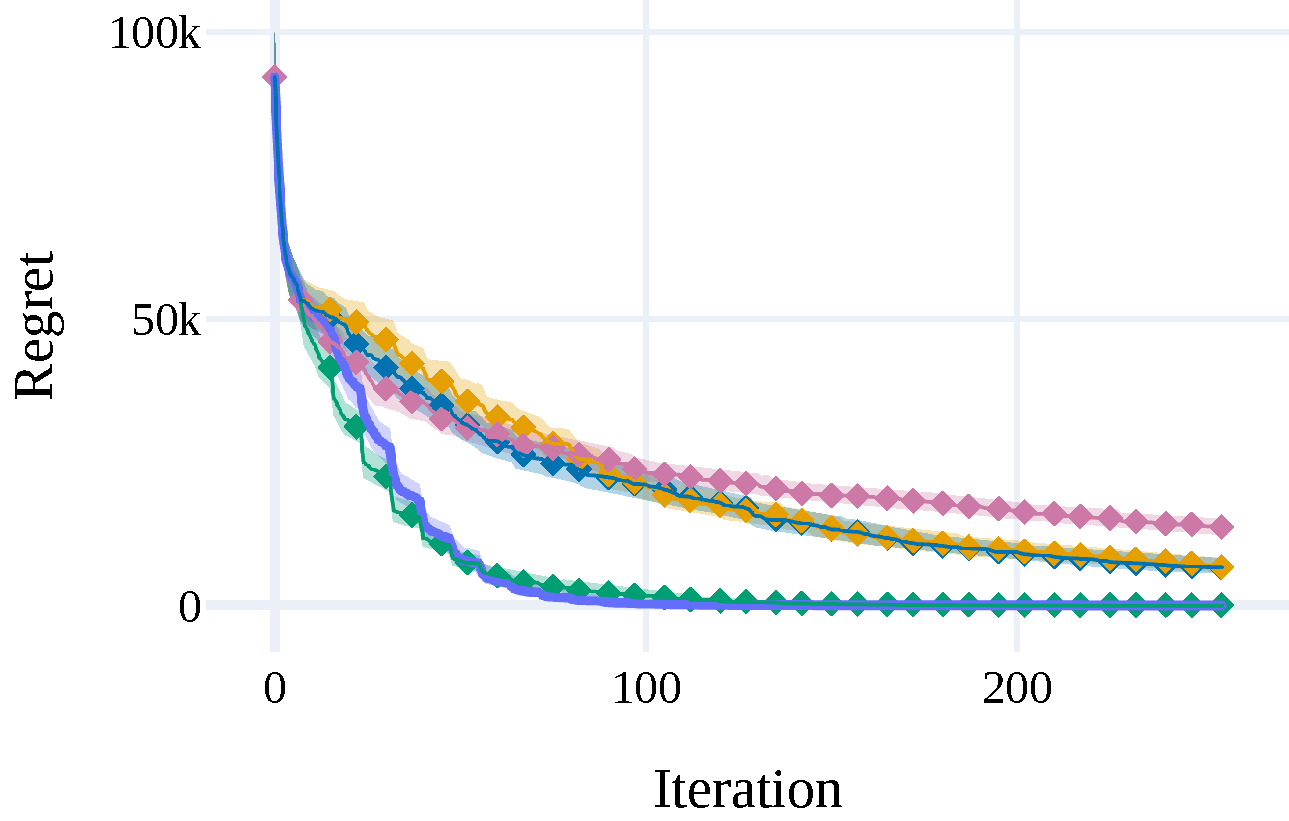
\includegraphics[scale=0.33]{figures/05/figs/figs/continuous/co_8_init_fbohachevsky_time.pdf}
        \caption{Hachevsky}
    \end{subfigure}
    \begin{subfigure}[t]{0.49\textwidth}
        \centering
        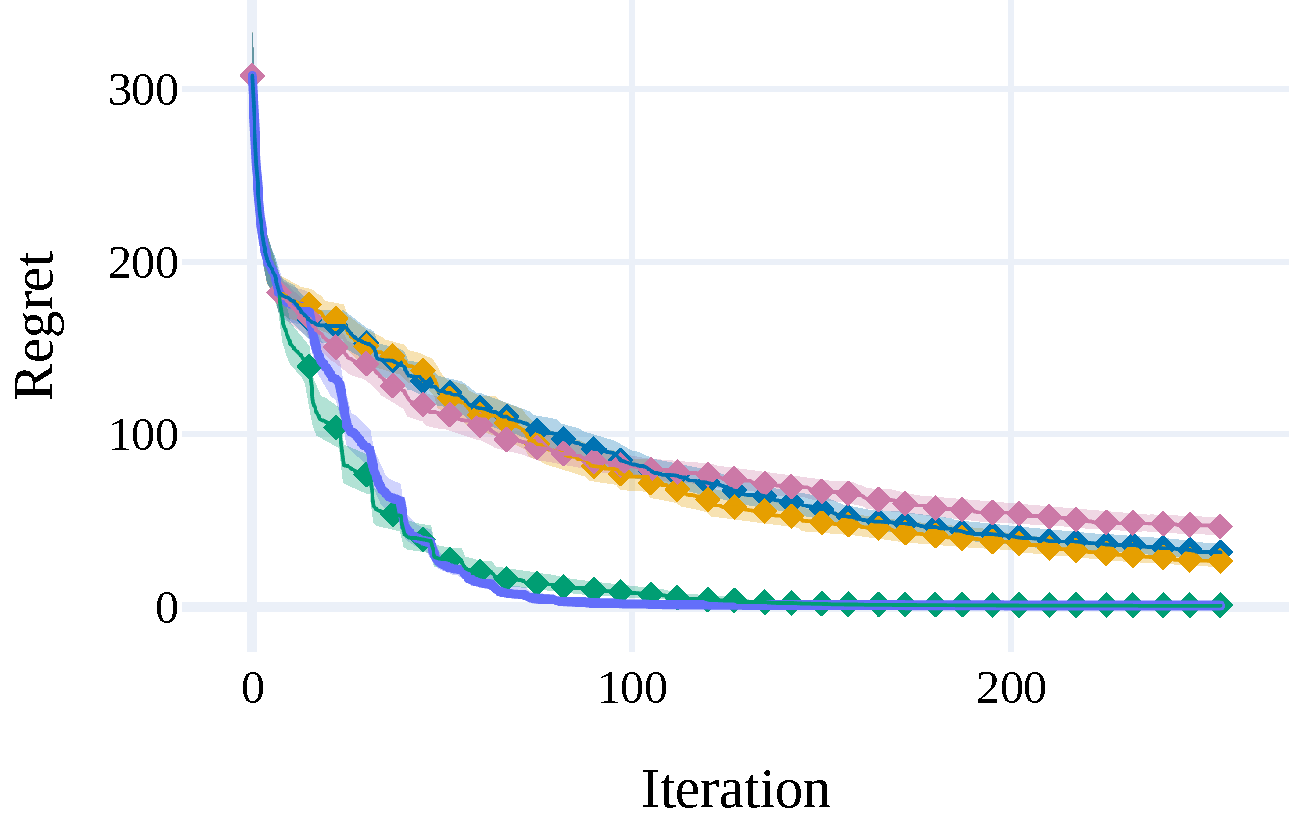
\includegraphics[scale=0.33]{figures/05/figs/figs/continuous/co_8_init_fgriewank_time.pdf}
        \caption{Griewank}
    \end{subfigure}
    \begin{subfigure}[t]{0.49\textwidth}
        \centering
        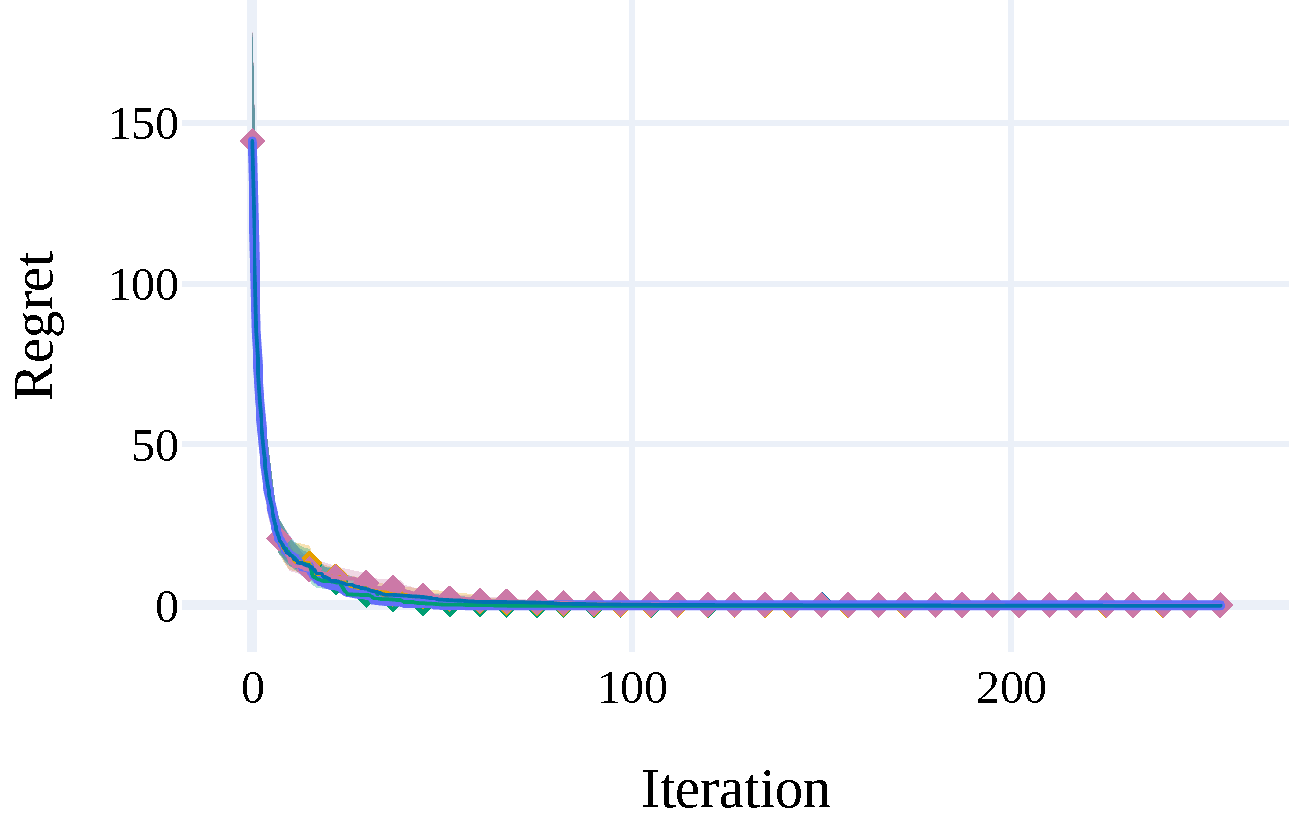
\includegraphics[scale=0.33]{figures/05/figs/figs/continuous/co_8_init_fhimmelblau_time.pdf}
        \caption{Himmelblau}
    \end{subfigure}
    \begin{subfigure}[t]{0.49\textwidth}
        \centering
        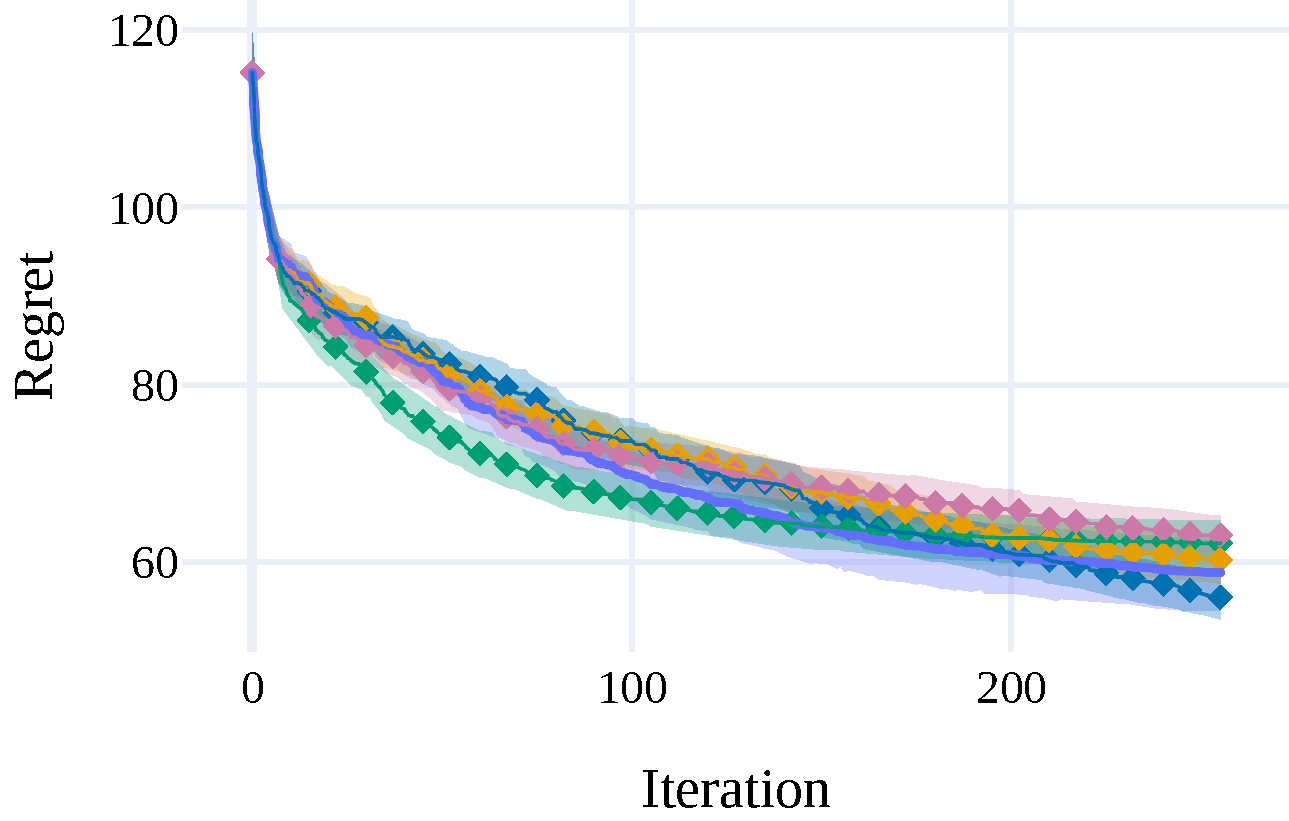
\includegraphics[scale=0.33]{figures/05/figs/figs/continuous/co_8_init_fschaffer_time.pdf}
        \caption{Schaffer}
    \end{subfigure}
    \begin{subfigure}[t]{0.49\textwidth}
        \centering
        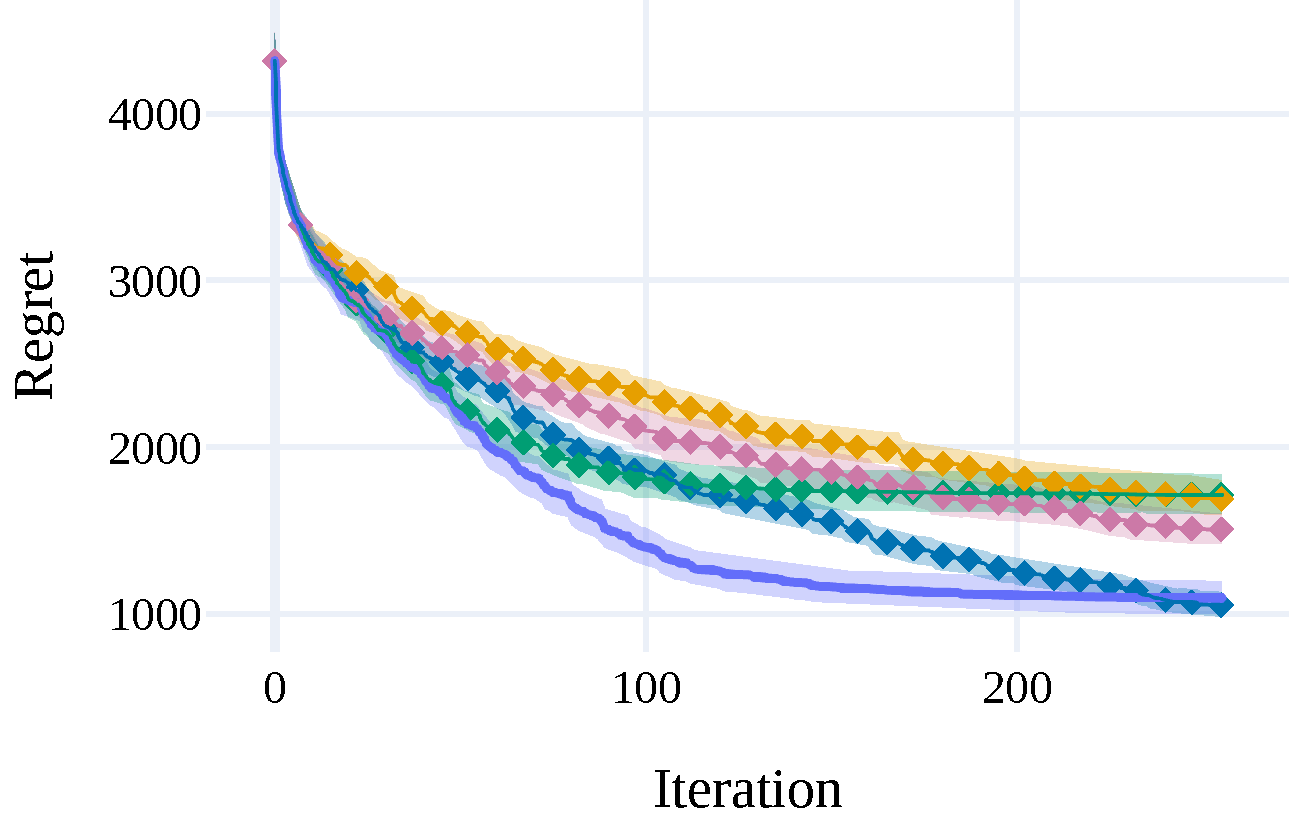
\includegraphics[scale=0.33]{figures/05/figs/figs/continuous/co_8_init_fschwefel_time.pdf}
        \caption{Schwefel}
    \end{subfigure}
        \begin{subfigure}[t]{\textwidth}
        \centering
        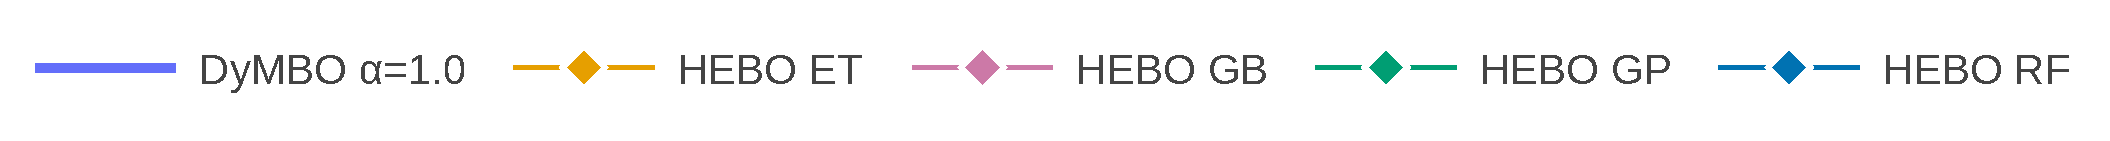
\includegraphics[scale=0.33]{figures/05/figs/figs/continuous/cont_legend.pdf}
        % \caption{}
    \end{subfigure}
    \caption{Convergence plots of \texttt{DyMBO} and single-surrogate HEBO baselines as a function of the number of evaluations on synthetic continuous functions in dimension $10$. \texttt{DyMBO} exhibits faster or competitive convergence, and an overall lower or comparable final regret.
    }
    \label{fig:ch05:synth-cont}
\end{figure*}

\subsection{HPOBench}
\label{sec:ch05:hpobench}

In addition to synthetic continuous functions, we empirically evaluated our method on HPOBench~\citep{EggEtAl21}, a collection of HPO benchmarks widely used in benchmarking studies.
Out of various raw, surrogate or tabular benchmark families included in HPOBench, we selected Random Forest and XGBoost as raw benchmarks for our evaluation.
These benchmarks are based on configuring hyperparameters of Random Forest and XGBoost models in their native implementations~\citep{PedEtAl11,CheGue16} on 20 publicly available datasets from the OpenML AutoML benchmark~\citep{GijEtAl19}.
The setup of experiments used here is the same as the default described in~\cref{sec:ch05:experiments}.

In~\cref{fig:ch05:hpobench}, we show the mean ranks of \texttt{DyMBO} and single-surrogate HEBO baselines on these two HPOBench problems.
\texttt{DyMBO} is ranked similarly to GB throughout the optimisation.
One possible reason for strong performance of GB compared to its performance on other benchmarks studied in this work is that uncertainty estimation of GB, based on quantile regression, is particularly well suited for for the structure of HPOBench.
In the later stages of optimisation, \texttt{DyMBO} becomes competitive with and even outperforms GB, since the dynamic weighting mechanism is increasingly able to recognise and incorporate accurate GB predictions as more observations become available.

Importantly, \texttt{DyMBO} consistently outperforms GP and RF, which are the strongest single-surrogate baselines on all other benchmarks studied in this work, demonstrating that dynamic surrogate tailoring still provides meaningful gains over these models even in a setting where GB dominates.
The relatively stable rank trajectories across all methods suggest that the relative ordering is established early in the optimisation and does not change drastically as the budget is consumed, with the exception of gradual convergence of \texttt{DyMBO} toward GB in the final stages of optimisation.

These results emphasise that \texttt{DyMBO} consistently performs well across various benchmarks with various search spaces and setups of experiments.

% A general observation across all methods is that the confidence bands are wide throughout the optimisation, indicating high variance in performance across benchmark instances. This suggests that the relative difficulty of these benchmarks varies considerably, and that no single method is universally dominant across all instances within this benchmark suite. 

\begin{figure*}
    \centering
    \begin{subfigure}[t]{0.49\textwidth}
        \centering
        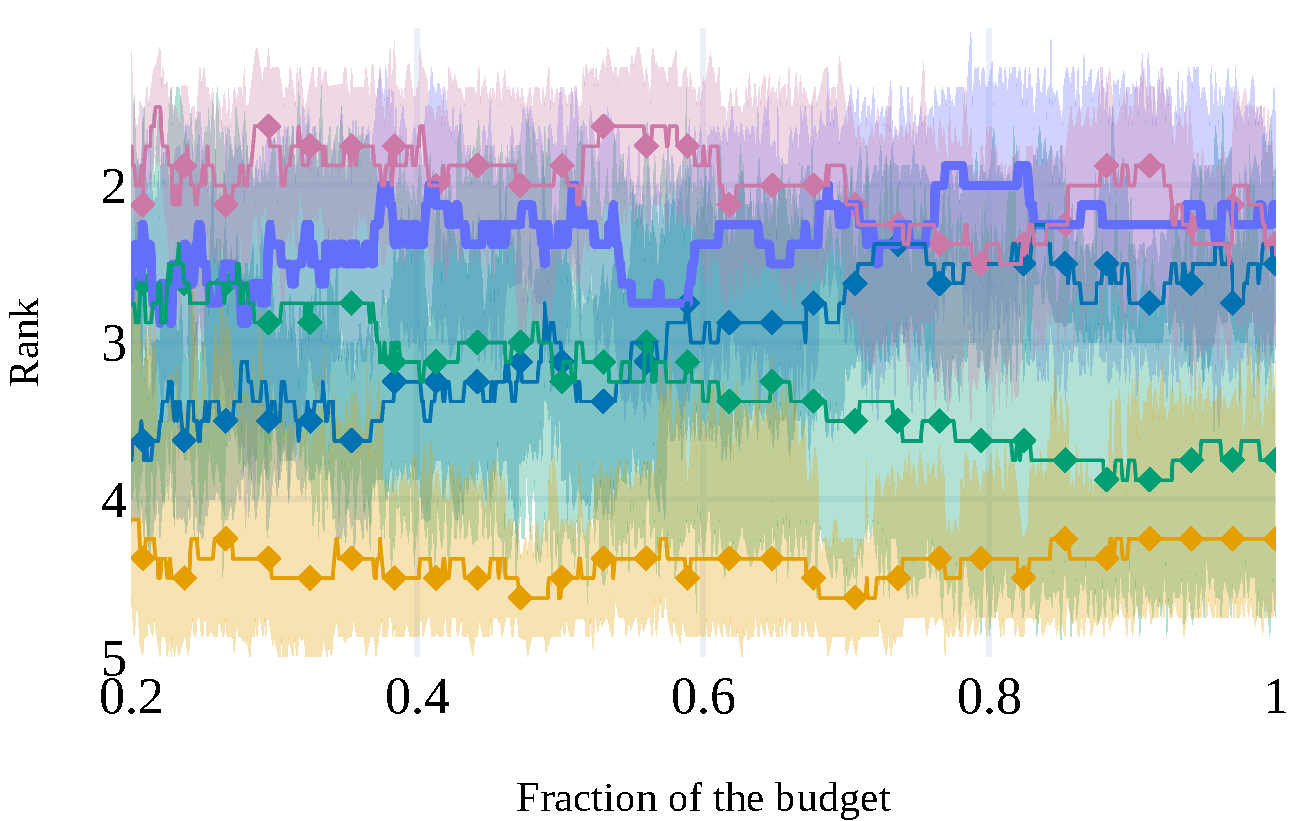
\includegraphics[scale=0.33]{figures/05/figs/figs/ranks/hpobench_all.pdf}
        % \caption{}
    \end{subfigure}
        \begin{subfigure}[t]{1.0\textwidth}
        \centering
        
\includegraphics[scale=0.33]{figures/05/figs/figs/ranks/hpobench_all_legend.pdf}
        % \caption{}
    \end{subfigure}
    \caption{
    Mean ranks of \texttt{DyMBO} and single-surrogate HEBO baselines as a function of the fraction of the wall-clock time budget on Random Forest and XGBoost raw benchmarks from HPOBench. \texttt{DyMBO} is ranked similarly to standalone GB surrogate, while outperforming GP and RF which are strongest single-surrogate candidates across all other benchmark scenarios.
    }
    \label{fig:ch05:hpobench}
\end{figure*}



\section{Conclusions, limitations and future work}
\label{sec:ch05:concl-fw}

% \changed{
In this work, we proposed a novel dynamic tailoring approach for surrogate models in BO-based HPO, spanning weighted ensembling and greedy selection. 
Our method assesses the accuracy of different surrogates throughout the optimisation process and dynamically determines whether to combine them or select among them by assigning and updating the model weights accordingly.
% }
We experimented with a wide variety of HPO benchmark tasks 
% \hh{minor changes:}
% \changed{
and baselines, and we found that, despite different mean ranks of BO with single surrogate models
% \er{what do we mean here? of the single methods, both DyMBO and all the other baselines? or of HEBO variants with the single surrogates?} 
on different benchmark categories, our method achieves a better mean rank across all benchmark categories. Furthermore, our method achieves better mean rank than all baselines, including single-surrogate methods as well as competing HPO frameworks.
As a rule of thumb, the variant of our method that is particularly well-performing is the one that does greedy dynamic selection ($\alpha = 1.0$) between a Gaussian process (whose initial weights are set at 0) and a random forest (whose initial weights are set at 1).
% }. % \er{Isn't this sentence a repetition of the previous one?}

Despite very promising results of our work, there is still room for improvement.
One limitation is the higher running time required to both train and evaluate the surrogate models and to optimise the acquisition function compared to a single-surrogate BO. %\er{Btw, is this a real problem if we only lose 150 s for 512 evaluations, where one evaluation takes 1 hour?}\hs{yes, because not all evaluations take 1 hour. Most ML benchmarks have shorter evaluation time} \er{ok, thanks :)}
We mitigate this by introducing dynamic pruning of surrogates, which substantially reduces the required running time.
% \changed{
However, dynamic pruning only reduces the running time required for acquisition function optimisation and still requires training multiple surrogate models at each iteration. Future work will focus on estimating the accuracy of the surrogate models without training them, thus reducing the computational cost of our method.

% \changed{
We  
% \hh{cut `also'}
note that our method has not yet been
% \hh{has not yet been} 
demonstrated to be robust against %\hh{better: against} 
the inclusion of a weak or poorly-suited surrogate in the portfolio.
While \texttt{DyMBO} is able to effectively hedge among a well-constructed, complementary portfolio, portfolio construction is currently not handled automatically by the method, but rather remains to be performed by the practitioner.
Extending the weighting mechanism to be robust to arbitrary or weak portfolio members is an important direction for future work.
% }

% \todo{add stacking, trace of ranks from the reviews}
Additionally, future work could consider alternative ways of looking at history beyond using the exponential moving average. For instance, it would be interesting to represent history via surrogate ranks, \emph{e.g.,} by means of a weighted average over the trace of ranks received by each of the surrogates, and to use those values as normalised ensemble weights.
Weights could also be learned using a standard stacking model, adapted such that computational overhead is avoided, \emph{e.g.},  by training stacking in each BO iteration.
% \changed{
Moreover, because \texttt{DyMBO} combines standard deviations from surrogates fit under different, model-specific approximations to the posterior, the resulting ensemble does not correspond to a single coherent Bayesian posterior, and a principled probabilistic treatment of this combination is left for future work.
% }
Furthermore, we found out that the choice of surrogate models our method considers to use has a strong impact on the performance, as we found that having sub-optimal models can cause to degraded performance compared to using only well-performing models.
% }

% Furthermore, we observe that the Gaussian process outperforms our method for very small budgets (less than 5 minutes). 
% This is in line with the fact that BO equipped with GP excels precisely in a very low-budget setting, as well as that our method requires higher time for the training additional surrogate models.

% Our method itself comes with a hyperparameter, the smoothing factor $\alpha$. 
% While different values of $\alpha$ work best with different target functions, we observed that using $\alpha=1.0$ works consistently well on all functions, regardless of the cost of function evaluations. 
% The impact of historical accuracy measurements thus seem to contribute only marginally when determining the weights.



We believe that our work presented opens several avenues for future research. 
Multi-fidelity approaches are very commonly used for HPO, especially in expensive tasks where each evaluation on full fidelity can take more than an hour. 
A natural extension of our method is to include multi-fidelity scenarios. 
Another promising direction is to learn in which scenarios (\emph{e.g.}, input dimensionality, phase of the optimisation) which surrogate model(s) work best and to create an ensemble by training only these specific models; 
in case a single surrogate model is chosen, the overhead of ensembling would thus be eliminated.


Overall, we believe that combining multiple surrogate models in BO is a promising direction for achieving better surrogate predictions, thus allowing for faster convergence and increased sample efficiency. 
\texttt{DyMBO} is the first method that dynamically leverages the potential of complementary surrogates within the BO procedure itself.